%%%%%%%%%%%%%%%%%%%%%%%%%%%%%%%%%%%%%%%%%%%%%%%%%%%%%%%%%%%%%%%%%%%%%%
% Lớp 11 | Dãy số. Cấp số cộng. Cấp số nhân | Cấp số nhân
% Dạng 1D2?3-8: Toán thực tế áp dụng cấp số nhân
% Số câu: 95  (sinh tự động bởi tach_cau.py; từ nay thầy sửa trực tiếp file này)
%%%%%%%%%%%%%%%%%%%%%%%%%%%%%%%%%%%%%%%%%%%%%%%%%%%%%%%%%%%%%%%%%%%%%%

%%%%%%%%%%%%%%%% TRẮC NGHIỆM 4 PHƯƠNG ÁN %%%%%%%%%%%%%%%%

% nguồn: Ok_Toan11_TracNghiem_Lan2
\begin{ex}%[1D2H3-8]%[ma:74c1aafa]
	Bạn A thả quả bóng cao su từ độ cao $10$ m theo phương thẳng đứng. Mỗi khi  chạm đất nó lại nảy lên theo phương thẳng đứng có độ cao bằng $\dfrac{3}{4}$ độ cao trước đó. Tính tổng quãng đường bóng đi được đến khi bóng dừng hẳn.
	 \choice
		{$40$  m}
		{\True $70$  m}
		{$50$ m} 
		{$80$ m} 
	\loigiai{Các quãng đường khi bóng đi xuống tạo thành một cấp số nhân lùi vô hạn có $u_1 = 10$  và $q = \dfrac{3}{4}$.\\
		 Tổng các quãng đường khi bóng đi xuống là $S = \dfrac{u_1}{1-q} = \dfrac{10}{1-\tfrac{3}{4}} = 40$.\\
	Tổng quãng đường bóng đi được đến khi bóng dừng hẳn $2S - 10 = 70$.} 
\end{ex}

% nguồn: Ok_Toan11_TracNghiem_Lan2
\begin{ex}%[1D2H3-8]%[ma:13b2a237]
	Dân số tỉnh Bình Phước theo điều tra vào ngày $1/1/2011$ là $905\,300$ người. Nếu  duy trì tốc độ tăng trưởng dân số không đổi là $10\%$ một năm thì đến $1/1/2020$ dân số của tỉnh Bình Phước là bao nhiêu?
	\choice 
		 {$22\,582\,927$}
		 {$20\,348\,115$}
		 {\True $2\,134\,650$}
		 {$11\,940\,591$}
	\loigiai{Sau $9$ năm thì số dân của tỉnh Bình Phước  là $905\,300\cdot 1{,}1^9 \approx 2\,134\,650$ người.}
\end{ex}

% nguồn: Ok_Toan11_TracNghiem_Lan2
\begin{ex}%[1D2H3-8]%[ma:7d4b98de]
	Người ta thiết kế một cái tháp gồm $11$ tầng. Diện tích bề mặt trên của mỗi tầng bằng nữa diện tích của mặt trên  của tầng ngay bên dưới và diện tích mặt trên của tầng $1$ bằng nửa diện tích của đế tháp. Tính diện tích mặt trên cùng biết diện tích đế tháp bằng $12\,288$ m$^2$.
	\choice 
		{\True $6$ m$^2$} 
		{$8$ m$^2$} 
		{$10$  m$^2$}
		{$12$  m$^2$}
	 \loigiai{
		Diện tích  bề mặt của mỗi tầng lập thành một cấp số nhân có công bội $q=\dfrac{1}{2}$ và $u_1=\dfrac{12\,288}{2}=6\,144$.
		Khi đó diện tích  mặt trên cùng là
		 \[u_{11}=u_1 q^{10}=\dfrac{6\,144}{2^{10}}=6.\]
	 }
\end{ex}

% nguồn: Ok_Toan11_TracNghiem_Lan2
\begin{ex}%[1D2V3-8]%[ma:5339105f]
	Tỷ lệ tăng dân số của tỉnh $M$ là $1{,}2\%$. Biết rằng số dân của tỉnh $M$ hiện nay là $2$ triệu người. Nếu  lấy kết quả chính xác đến hàng nghìn thì sau $9$ năm nữa số dân của tỉnh $M$ sẽ là bao nhiêu?
	\choice 
		{$10\,320$  nghìn người}
		{$3\,000$  nghìn người}
		{\True $2\,227$ nghìn  người}
		{$2\,300$ nghìn người} 
	 \loigiai{
		Đặt $P_0=2\,000\,000=2\cdot 10^6$  và $r=1{,}2\%=0{,}012$.\\
		Gọi $P_n$ là số dân của tỉnh $M$ sau $n$ năm  nữa.\\
		Ta có $P_{n+1}=P_n+P_n r=P_n  \left(1+r\right)$.\\
		Suy ra $\left(P_n \right)$ là một cấp số nhân với  số hạng đầu $P_0$ và công bội $q=1+r$.\\
		Do đó số dân của tỉnh $M$  sau $10$ năm nữa là $P_9=M_0 \left(1+r\right)^9=2\cdot 10^6\cdot \left(1,012\right)^{10} \approx 2\,227\,000$.
	} 
\end{ex}

% nguồn: Ok_Toan11_TracNghiem_Lan2
\begin{ex}%[1D2V3-8]%[ma:00728a8f]
	Từ độ cao $55{,}8$ m  của tháp nghiêng Pisa nước Italia người ta thả một quả bóng cao su chạm xuống đất. Giả sử mỗi lần chạm đất quả bóng lại nảy lên độ cao bằng $\dfrac{1}{10}$ độ cao mà quả bóng đạt trước đó. Tổng độ dài hành trình của quả bóng được thả từ lúc ban đầu cho đến khi nó nằm yên trên mặt đất thuộc khoảng nào trong các khoảng sau đây?
	 \tikzset{
	 ex_markstyle/.style={},
	ex_mark/.style n args={1}{decoration={  markings,
	mark=  at position 0.5 with
	with{ 
	\ifnum#1=1 
	\draw[ex_markstyle] (0pt,-2pt)  -- (0pt,2pt);
	\fi 
	 \ifnum#1=2
	\draw[ex_markstyle] (-1pt,-2pt)  -- (-1pt,2pt);
	 \draw[ex_markstyle] (1pt,-2pt) -- (1pt,2pt);
	\fi 
	 \ifnum#1=3
	\draw[ex_markstyle] (-2pt,-2pt)  -- (-2pt,2pt);
	\draw[ex_markstyle] (0pt,-2pt)  -- (0pt,2pt);
	\draw[ex_markstyle] (2pt,-2pt)  -- (2pt,2pt);
	\fi 
	\ifnum#1=4 
	 \draw[ex_markstyle] (-1pt,-1pt) -- (1pt,1pt);
	\draw[ex_markstyle]  (-1pt,1pt) -- (1pt,-1pt);
	 \fi
	} }, 
	pic actions/.append code=\tikzset{postaction=decorate}},
	 }
	\definecolor{lightcornflowerblue}{rgb}{0.6,  0.81, 0.93}
	\definecolor{cadmiumgreen}{rgb}{0.0,  0.42, 0.24}
	 \definecolor{trueblue}{rgb}{0.0, 0.45, 0.81}
	\definecolor{tumbleweed}{rgb}{0.87, 0.67,  0.53}
	\begin{center}
		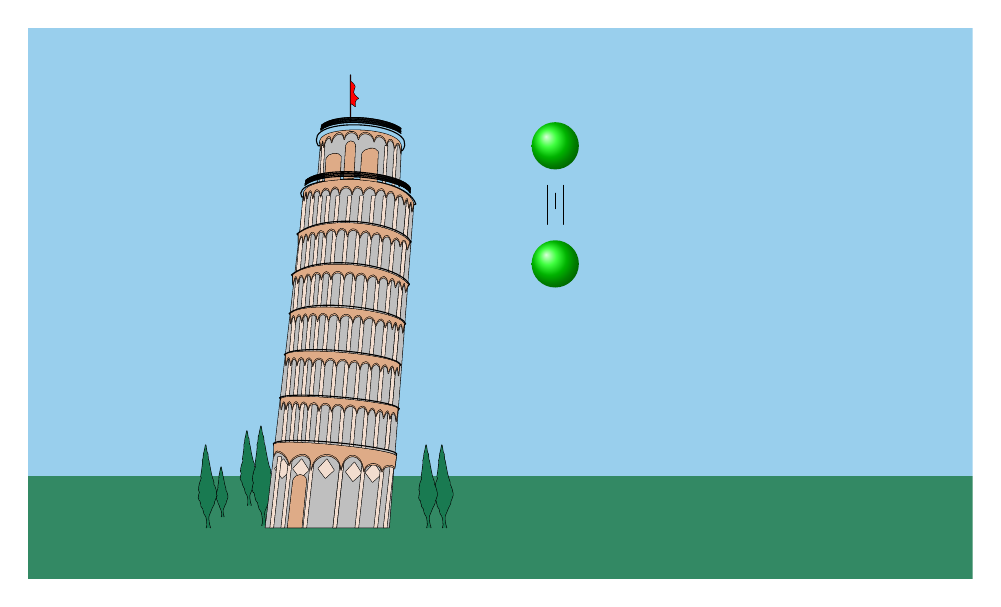
\begin{tikzpicture}[line join=round,line cap=round,scale=1,transform shape]
				\clip (-4,-3.5) rectangle  (8,3.5);
				\tikzset{thap/.pic={ 
				 \def\T{
					 (-.88,-1.78)
					..controls +(40:.17)  and +(120:.1).. (.686,-1.91)--(.68,-1.94)
					..controls +(120:.1)  and +(40:.12).. (-.87,-1.81)
					 --cycle
					(-.8,-1.2) 
					..controls +(40:.14) and +(120:.14).. (.72,-1.34)--(.7,-1.36) 
					..controls +(120:.1) and +(40:.12).. (-.78,-1.23) 
					--cycle 
					(-.74,-.65) 
					..controls +(40:.22) and +(120:.17).. (.74,-.78)--(.72,-.8) 
					..controls +(120:.15)  and +(40:.15).. (-.72,-.67)
					--cycle 
					(-.68,-.13) 
					..controls  +(40:.34) and +(110:.2).. (.8,-.26)--(.78,-.28)
					..controls +(110:.17) and +(40:.27).. (-.66,-.15) 
					--cycle 
					(-.65,.36) 
					..controls +(40:.44)  and +(120:.3).. (.85,.24)--(.83,.22)
					..controls +(130:.35)  and +(40:.35).. (-.63,.34)
					--cycle 
					(-.58,.88) 
					 ..controls +(40:.44) and +(120:.3).. (.87,.78)--(.85,.76)
					..controls +(130:.35) and +(40:.35)..  (-.56,.86)
					 --cycle
					(-.52,1.35) 
					 ..controls +(120:.32) and +(110:.47).. (.93,1.26)--(.9,1.25)
					..controls  +(110:.43) and +(110:.27).. (-.49,1.35)
					 --cycle
					(-.31,2) 
					..controls +(120:.47) and +(55:.46).. (.76,1.94)--(.74,1.94) 
					..controls +(75:.31) and +(115:.28)..  (-.28,2)
					--cycle 
					(-.48,1.5) 
					..controls  +(40:.33) and +(110:.2).. (.86,1.4)
					(-.476,1.52) 
					..controls +(40:.33) and +(110:.2).. (.86,1.42) 
					 (-.472,1.54)
					 ..controls +(40:.33) and +(110:.2).. (.86,1.44)
					(-.468,1.56) 
					..controls +(40:.33)  and +(110:.2).. (.86,1.46)
					(-.28,2.2) 
					..controls +(40:.27)  and +(140:.2).. (.74,2.16)
					 (-.276,2.22)
					..controls +(40:.27)  and +(140:.2).. (.74,2.18)
					 (-.272,2.24)
					..controls +(40:.27) and +(140:.2)..  (.74,2.2)
					(-.268,2.26) 
					 ..controls +(40:.27) and +(140:.2).. (.74,2.22);}
				\draw  \T;
					 }}
				\tikzset{rao/.pic={ 
				 \def\R{
					(-.48,1.5) 
					..controls +(40:.33) and  +(110:.2).. (.86,1.4)
					 (-.476,1.52)
					..controls  +(40:.33) and +(110:.2).. (.86,1.42)
					 (-.472,1.54)
					..controls +(40:.33) and +(110:.2).. (.86,1.44) 
					 (-.468,1.56)
					..controls +(40:.33) and +(110:.2).. (.86,1.46) 
					(-.28,2.2) 
					..controls +(40:.27) and +(140:.2)..  (.74,2.16)
					(-.276,2.22) 
					..controls +(40:.27)  and +(140:.2).. (.74,2.18)
					(-.272,2.24) 
					..controls  +(40:.27) and +(140:.2).. (.74,2.2)
					 (-.268,2.26)
					..controls +(40:.27) and +(140:.2)..  (.74,2.22);}
				 \draw \R;
					 }}
				 \tikzset{co/.pic={
				 \def\C{
					 (0.1,2.3)--(.1,2.9)
					(.1,2.82) 
					..controls +(-40:.2)  and +(140:.22).. (.2,2.6)
					..controls  +(-60:0) and +(100:.1)..(.16,2.5)
					..controls  +(140:.1) and +(-30:0).. (.1,2.53)--cycle;}
				 \draw \C;
				\fill[red]  \C;
					 }}
				 \tikzset{cong0/.pic={
				 \def\D0{
					(.68,-1.96) 
					..controls +(120:.1)  and +(40:.12).. (-.87,-1.81)--
					(-.87,-1.94) 
					..controls +(80:.12) and  +(95:0.12).. (-.68,-2.06)
					..controls +(80:.12) and +(85:0.3).. (-.4,-2.12) 
					 ..controls +(80:.25) and +(95:0.25).. (-.02,-2.12)
					..controls +(80:.25) and +(95:0.25)..  (.27,-2.14)
					..controls +(80:.12) and  +(95:0.12).. (.5,-2.14)
					..controls +(70:.12)  and +(95:0.02).. (.66,-2.1)--cycle;}
				\draw  \D0;
				\fill[tumbleweed]  \D0;
					}} 
				\tikzset{cong1/.pic={ 
				 \def\D1{
					(.7,-1.36) 
					 ..controls +(120:.1) and +(40:.12).. (-.78,-1.23)--
					(-.78,-1.35) 
					..controls +(80:.12) and  +(95:0.12).. (-.72,-1.35)
					..controls +(80:.12) and  +(95:0.12).. (-.64,-1.35)
					..controls +(80:.12)  and +(95:0.12).. (-.55,-1.35)
					 ..controls +(80:.12) and +(95:0.12).. (-.44,-1.36)
					..controls  +(80:.12) and +(95:0.12).. (-.3,-1.37)
					..controls +(80:.12)  and +(95:0.12).. (-.14,-1.38)
					 ..controls +(80:.12) and +(95:0.12).. (0.02,-1.39)
					..controls +(80:.12)  and +(95:0.12).. (0.18,-1.4)
					..controls  +(80:.12) and +(95:0.12).. (0.32,-1.42)
					 ..controls +(70:.12) and +(95:0.12).. (0.42,-1.44)
					..controls +(70:.12) and  +(95:0.12).. (0.52,-1.46)
					..controls  +(70:.12) and +(95:0.12).. (0.6,-1.47)
					 ..controls +(70:.12) and +(95:0.12).. (0.68,-1.5)--cycle;}
				 \draw \D1;
				\fill[tumbleweed] \D1; 
					 }}
				\tikzset{cong2/.pic={ 
				 \def\D2{
					(.72,-.8) 
					..controls +(120:.15) and +(40:.15)..  (-.72,-.67)--
					 (-.72,-.79)
					..controls +(80:.12) and  +(95:0.12).. (-.66,-.79)
					..controls +(80:.12) and +(95:0.12).. (-.58,-.79) 
					..controls +(80:.12) and  +(95:0.12).. (-.48,-.79)
					..controls +(80:.12) and  +(95:0.12).. (-.38,-.8)
					..controls +(80:.12) and +(95:0.12).. (-.23,-.8) 
					..controls  +(80:.12) and +(95:0.12).. (-0.08,-.81)
					..controls +(80:.12) and  +(95:0.12).. (0.08,-.82)
					..controls  +(80:.12) and +(95:0.12).. (0.22,-.84)
					..controls +(80:.12)  and +(95:0.12).. (0.36,-.85)
					..controls +(70:.12) and +(95:0.12).. (0.48,-.87) 
					..controls +(70:.12) and  +(95:0.12).. (0.58,-.89)
					..controls +(70:.12) and +(95:0.12).. (0.66,-.9) 
					..controls +(70:.12)  and +(95:0.12).. (0.71,-.92)--cycle;}
				\draw \D2; 
				\fill[tumbleweed]  \D2;
					 }}
				\tikzset{cong3/.pic={ 
				\def\D3{ 
					(.78,-.28) 
					..controls  +(110:.17) and +(40:.27).. (-.66,-.15)--
					 (-.66,-.26)
					..controls +(80:.12) and  +(95:0.12).. (-.6,-.25)
					 ..controls +(80:.12) and +(95:0.12).. (-.52,-.24)
					 ..controls +(80:.12) and +(95:0.12).. (-.44,-.23)
					..controls +(80:.12) and +(95:0.12)..  (-.32,-.23)
					..controls +(80:.12)  and +(95:0.12).. (-.18,-.23)
					..controls +(80:.12) and +(95:0.12)..  (-.04,-.24)
					..controls +(80:.12)  and +(95:0.12).. (0.13,-.25)
					..controls +(80:.12) and +(95:0.12)..  (0.26,-.26)
					..controls +(70:.12) and  +(95:0.12).. (0.42,-.29)
					..controls  +(70:.12) and +(95:0.12).. (0.54,-.31)
					..controls +(70:.12) and +(95:0.12)..  (0.63,-.33)
					..controls +(70:.12) and  +(95:0.12).. (0.7,-.35)
					..controls  +(70:.12) and +(95:0.12).. (0.765,-.38)--cycle;}
				 \draw \D3;
				\fill[tumbleweed]  \D3;
					}} 
				\tikzset{cong4/.pic={ 
				 \def\D4{
					 (.83,.22)
					 ..controls +(130:.35) and +(40:.35).. (-.63,.34)--
					 (-.63,.23)
					..controls  +(80:.12) and +(95:0.12).. (-.57,.25)
					 ..controls +(80:.12) and +(95:0.12).. (-.49,.26)
					..controls  +(80:.12) and +(95:0.12).. (-.4,.28)
					..controls +(80:.12) and  +(95:0.12).. (-.27,.3)
					..controls +(80:.12) and +(95:0.12).. (-.15,.3) 
					..controls  +(80:.12) and +(95:0.12).. (0.02,.3)
					..controls  +(80:.12) and +(95:0.12).. (0.16,.29)
					..controls +(80:.12)  and +(95:0.12).. (0.31,.27)
					..controls  +(70:.12) and +(95:0.12).. (0.45,.25)
					..controls +(70:.12) and +(95:0.12).. (0.58,.23) 
					..controls +(70:.12) and +(95:0.12).. (0.67,.2) 
					..controls  +(70:.12) and +(95:0.12).. (0.75,.17)
					..controls +(70:.12)  and +(95:0.12).. (0.8,.14)--cycle;}
				 \draw \D4;
				\fill[tumbleweed]  \D4;
					}} 
				 \tikzset{cong5/.pic={
				\def\D5{ 
					(.85,.76) 
					..controls +(130:.35) and +(40:.35).. (-.56,.86)-- 
					 (-.56,.74)
					..controls +(80:.12)  and +(95:0.12).. (-.5,.77)
					..controls +(80:.12) and +(95:0.12)..  (-.44,.79)
					..controls +(80:.12)  and +(95:0.12).. (-.34,.81)
					..controls +(80:.12) and +(95:0.12)..  (-.22,.83)
					..controls  +(80:.12) and +(95:0.12).. (-0.08,.85)
					..controls +(80:.12)  and +(95:0.12).. (0.06,.85)
					..controls +(80:.12) and +(95:0.12).. (0.22,.83) 
					..controls +(70:.12) and +(95:0.12).. (0.36,.81) 
					..controls  +(70:.12) and +(95:0.12).. (0.5,.78)
					..controls +(70:.12) and +(95:0.12)..  (0.62,.74)
					..controls +(70:.12) and +(95:0.12)..  (0.73,.72)
					..controls +(70:.12) and +(95:0.12).. (0.82,.68)--cycle;} 
				 \draw \D5;
				\fill[tumbleweed] \D5; 
					}} 
				\tikzset{cong6/.pic={ 
				\def\D6{ 
					 (.9,1.25)
					..controls +(110:.43) and +(110:.27).. (-.49,1.35)-- 
					(-.49,1.3) 
					..controls  +(80:.12) and +(95:0.12).. (-.45,1.33)
					..controls  +(80:.12) and +(95:0.12).. (-.38,1.33)
					 ..controls +(80:.12) and +(95:0.12).. (-.28,1.35)
					..controls +(80:.12)  and +(95:0.12).. (-.16,1.37)
					..controls  +(80:.12) and +(95:0.12).. (-0.04,1.38)
					..controls +(80:.12)  and +(95:0.12).. (0.12,1.38)
					..controls +(80:.12)  and +(95:0.12).. (0.26,1.38)
					..controls +(70:.12) and +(95:0.12).. (0.42,1.37) 
					..controls +(70:.12)  and +(95:0.12).. (0.55,1.34)
					..controls +(70:.12) and  +(95:0.12).. (0.67,1.3)
					..controls +(70:.12) and +(95:0.12)..  (0.78,1.25)
					..controls  +(70:.12) and +(95:0.12).. (0.84,1.21)
					 ..controls +(70:.12) and +(95:0.12).. (0.88,1.16)--cycle;}
				 \draw \D6;
				 \fill[tumbleweed] \D6;
					}} 
				 \tikzset{cong7/.pic={
				 \def\D7{
					(.74,1.94) 
					..controls +(75:.31) and +(115:.28)..  (-.28,2)--
					(-.28,1.94) 
					..controls +(80:.12) and  +(95:0.12).. (-.24,1.98)
					..controls +(80:.12) and +(95:0.12)..  (-.14,2.04)
					..controls +(80:.12) and +(95:0.12).. (0.02,2.08) 
					..controls +(80:.12) and +(95:0.12).. (0.2,2.08) 
					..controls +(80:.12) and +(95:0.12)..  (0.4,2.05)
					..controls +(80:.12) and +(95:0.12)..  (0.56,2)
					..controls +(80:.12) and  +(95:0.12).. (0.66,1.96)
					..controls +(70:.12)  and +(95:0.12).. (0.74,1.9)--cycle;}
				 \draw \D7;
				\fill[tumbleweed] \D7; 
					}} 
				 \tikzset{cua/.pic={
				 \def\W{
					 (-.7,-2.85)--(-.63,-2.25)
					..controls +(70:.1) and  +(100:.1).. (-.46,-2.25)--(-.52,-2.85)
					--cycle;} 
				\draw \W; 
				\fill[tumbleweed]  \W;
					}} 
				\tikzset{vien/.pic={ 
				\def\V{ 
					 (.9,1.25)
					..controls +(110:.43) and +(110:.27)..  (-.49,1.35)--(-.98,-2.85)--(.59,-2.85)--cycle
					(.74,1.94) 
					..controls +(75:.31)  and +(115:.28).. (-.28,2)--(-.32,1.54)
					..controls +(115:.2)  and +(75:.13).. (.72,1.48)--cycle;}
				\draw  \V;
				\fill[gray!50!] \V; 
					 }}
				 \tikzset{soc/.pic={
				\def\S{ 
					(.82,1.36)--(.54,-1.85)--(.58,-1.85)--(.86,1.36) 
					 --cycle;}
				 \draw \S;
				 \fill[tumbleweed!40!] \S;
					 }}
				\tikzset{soc2/.pic={ 
				\def\S{ 
					 (.54,-1.95)--(.44,-2.85)--(.48,-2.85)--(.58,-1.95)
					--cycle;} 
				\draw \S; 
				\fill[tumbleweed!40!] \S; 
					}} 
				 \tikzset{soc3/.pic={
				 \def\S{
					(.54,2)--(.57,2)--(.54,1.5)--(.51,1.5) 
					--cycle 
					(.66,2)--(.69,2)--(.66,1.5)--(.63,1.5) 
					 --cycle
					 (-.26,2)--(-.23,2)--(-.26,1.5)--(-.29,1.5)
					--cycle;} 
				 \draw \S;
				 \fill[tumbleweed!40!] \S;
					 }}
				\tikzset{thoi/.pic={ 
				 \def\T{
					(0.15,-1.98)--(.24,-2.12)--(0.13,-2.22)--(0.04,-2.1) 
					 --cycle;}
				 \draw \T;
				\fill[tumbleweed!40!] \T; 
					 }}
				\tikzset{cay/.pic={ 
				\def\T{ 
					 (-1.73,-2.85)
					..controls +(40:.03) and +(40:.01)..  (-1.74,-2.7)
					..controls +(140:.04) and +(60:.02).. (-1.78,-2.6) 
					 ..controls +(140:.04) and +(60:.02).. (-1.8,-2.55)
					..controls +(100:.03) and +(70:.02)..  (-1.82,-2.5)
					 ..controls +(140:.04) and +(60:.02).. (-1.815,-2.4)
					 ..controls +(140:.04) and +(60:.02).. (-1.818,-2.3)
					..controls +(85:.03) and  +(-30:.03).. (-1.8,-2.2)
					 ..controls +(80:.04) and +(50:.02).. (-1.78,-2)
					 ..controls +(60:.04) and +(120:.02).. (-1.76,-1.9)
					..controls +(80:.03) and  +(-100:.02).. (-1.74,-1.8)
					..controls +(80:.01) and +(-100:.02)..  (-1.72,-1.9)
					 ..controls +(60:.02) and +(-120:.02).. (-1.7,-2)
					..controls +(-80:.02) and  +(110:.03).. (-1.66,-2.2)
					..controls +(-100:.02)  and +(60:.03).. (-1.64,-2.3)
					..controls +(-30:.02)  and +(70:.02).. (-1.6,-2.44)
					..controls  +(-100:.02) and +(70:.02).. (-1.63,-2.52)
					..controls  +(-60:.02) and +(70:.01).. (-1.66,-2.6)
					..controls +(60:.01) and +(70:.02).. (-1.7,-2.7) 
					 ..controls +(-120:.02) and +(120:.03).. (-1.68,-2.85);}
				\draw \T; 
				 \fill[cadmiumgreen!90!] \T;
					 }}
				\fill[cadmiumgreen!80!] (-4,-3.5)  rectangle (8,-2.2);
				\fill[lightcornflowerblue] (-4,3.5)  rectangle (8,-2.2);
				 \path
					(0,0)  pic[scale=1]{cay}
					 (.35,0) pic[scale=.9]{cay}
					(1.05,0.6) pic[scale=1.2]{cay} 
					 (-.5,-1) pic[scale=.6]{cay}
					(3,0)  pic[scale=1]{cay}
					(2.8,0) pic[scale=1]{cay} 
					(0,0) pic[scale=1]{vien} 
					(0,0)  pic[scale=1]{soc}
					(0,0)  pic[scale=1]{soc}
					 (-.15,0) pic[scale=1]{soc}
					(-.3,0)  pic[scale=1]{soc}
					 (-.45,0) pic[scale=1]{soc}
					(-.6,0)  pic[scale=1]{soc}
					 (-.75,0) pic[scale=1]{soc}
					 (-.9,0) pic[scale=1]{soc}
					(-1.02,0) pic[scale=1]{soc} 
					 (-1.12,0) pic[scale=1]{soc}
					(-1.22,0) pic[scale=1]{soc} 
					(-1.32,0) pic[scale=1]{soc} 
					(0,0)  pic[scale=1]{soc3}
					(0,0)  pic[scale=1]{thap}
					(0,0) pic[scale=1]{co} 
					(.4,3.6) pic[scale=.7,rotate=3]{cua} 
					(.8,3.6) pic[scale=1.2,rotate=7,yscale=.6]{cua} 
					(.3,3.4) pic[scale=1.1,rotate=7,yscale=.6]{cua} 
					 (0,-.04) pic[scale=1]{thoi}
					(0.25,-.05)  pic[scale=1]{thoi}
					 (-0.35,0) pic[scale=1]{thoi}
					(-.67,0) pic[scale=1]{thoi} 
					(-.9,0)  pic[scale=1]{thoi}
					(-1.22,0) pic[scale=1]{soc2} 
					(-1.36,0)  pic[scale=1]{soc2}
					(-.94,0) pic[scale=1]{soc2} 
					(-.56,0)  pic[scale=1]{soc2}
					 (-.56,0) pic[scale=1]{soc2}
					 (.08,0) pic[scale=1]{soc2}
					 (-.04,0) pic[scale=1]{soc2}
					(-.28,0) pic[scale=1]{soc2} 
					 (0,0) pic[scale=1]{cong0}
					(0,0.02)  pic[scale=1]{cong0}
					(0,0) pic[scale=1]{cong1} 
					(0,0.02) pic[scale=1]{cong1} 
					(0,0)  pic[scale=1]{cong2}
					 (0,0.02) pic[scale=1]{cong2}
					(0,0) pic[scale=1]{cong3} 
					(0,0.02) pic[scale=1]{cong3} 
					 (0,0) pic[scale=1]{cong4}
					(0,0.02)  pic[scale=1]{cong4}
					(0,0)  pic[scale=1]{cong5}
					 (0,0.02) pic[scale=1]{cong5}
					(0,0) pic[scale=1]{cong6} 
					 (0,0.02) pic[scale=1]{cong6}
					(0,0)  pic[scale=1]{cong7}
					(0,0.02)  pic[scale=1]{cong7}
					(0,0) pic[scale=1]{cua} 
					(0,0)  pic[scale=1]{rao};
				\shade[ball color=green]  (2.7,2) circle (0.3cm);
				\shade[ball  color=green] (2.7,0.5) circle (0.3cm);
				\draw[very thin] (2.7,1.4)--(2.7,1.2) 
					 (2.8,1.5)--(2.8,1)
					 (2.6,1.5)--(2.6,1);
			\end{tikzpicture}
	\end{center}
	\choice 
		{\True  $\left(67\;\mathrm{m};69\;\mathrm{m}\right)$}
		 {$\left(60\;\mathrm{m};63\;\mathrm{m}\right)$}
		{$\left(64\;\mathrm{m};66\;\mathrm{m}\right)$} 
		{$\left(69\;\mathrm{m};72\;\mathrm{m}\right)$} 
	 \loigiai{
		Gọi $h_n$  là độ dài đường đi của quả bóng ở lần rơi xuống thứ $n\left(n\in \mathbb{N}^{*} \right)$.\\
		Gọi $\ell_n$ là độ dài đường đi của quả bóng ở lần nảy lên thứ $n\left(n\in \mathbb{N}^{*} \right)$.\\ 
		Theo bài ra ta có $h_1=55{,}8$, $\ell_1=\dfrac{1}{10}\cdot 55{,}8=5{,}58$ và các dãy số $\left(h_n  \right)$, $\left(\ell_n \right)$ là các cấp số nhân lùi vô hạn với công bội $q=\dfrac{1}{10}\cdot$\\
		Từ đó ta suy ra tổng độ dài đường đi  của quả bóng là
		\[S=\dfrac{h_1}{1-\dfrac{1}{10}}+\dfrac{\ell_1}{1-\dfrac{1}{10}}=\dfrac{10}{9} \left(h_1+\ell_1  \right)=68{,}2\;(\mathrm{m}).\]
	} 
\end{ex}

% nguồn: Ok_Toan11_TracNghiem_Lan2
\begin{ex}%[1D2V3-8]%[ma:c44c1dc0]
	Trên một bàn cờ vua kích thước $8\times 8$ người ta đặt số hạt thóc theo cách như sau. Ô thứ nhất đặt một hạt thóc, ô thứ hai đặt hai hạt thóc, các ô tiếp theo đặt số hạt thóc gấp  đôi ô đứng liền kề trước nó. Hỏi phải tối thiểu từ ô thứ bao nhiêu để tổng số hạt thóc từ ô đầu tiên đến ô đó lớn hơn $20\,172\,018$ hạt thóc.
	\choice 
		{$26$} 
		{$23$} 
		{$24$} 
		 {\True $25$}
	 \loigiai{
		Số thóc ở ô sau gấp đôi ở ô trước, đặt $u_n$ là số thóc ở ô thứ $n$ thì số thóc ở mỗi ô sẽ lập thành một cấp  số nhân có
		 $\heva{&u_1=1=2^0\\&u_{n+1}=2u_n=2^n.}$\\
		Khi đó tổng số thóc  từ ô đầu tới ô thứ $k$ là $S_k=u_1+u_2+\cdots+u_k=1+2^1+\cdots+2^{k-1}$.\\
		Vậy  $S_k=\dfrac{2^k-1}{2-1}=2^k-1$.\\
		Theo đề ta có $2^k-1> 20\,172\,018\Leftrightarrow 2^k > 20\,172\,019$.\\ 
		Do  $2^{24}<20\,172\,019<2^{25} \Rightarrow k=25$.\\
		 Vậy phải lấy tối thiểu từ ô thứ $25$.
	 }
\end{ex}

% nguồn: Ok_Toan11_TracNghiem_Lan2
\begin{ex}%[1D2V3-8]%[ma:01704c8e]
	Với hình vuông $A_1 B_1 C_1 D_1$ như hình vẽ bên, cách tô màu như  phần gạch sọc được gọi là cách tô màu \lq\lq đẹp\rq\rq. Một nhà thiết kế tiến hành tô màu cho một hình vuông như hình bên, theo quy trình sau
	\begin{center}
		\begin{tikzpicture}[thick,scale=1,nodes={scale=1}]
				\def\a{4} 
				\path 
					(0:0) coordinate (D_1) 
					++(0:\a) coordinate  (C_1)
					 ++(90:\a) coordinate (B_1)
					++(180:\a)  coordinate (A_1);
				 \draw (A_1)--(B_1)--(C_1)--(D_1)--cycle;
				\foreach \x/ \goc in {A_1/135,B_1/45,C_1/-45,D_1/-135} \fill (\x) circle  (1pt)
					($(\x)+(\goc:3mm)$) node {$\x$}; 
				 \path
					 (\a/3,\a/3) coordinate (D_2)
					++(0:\a/3) coordinate  (C_2)
					++(90:\a/3) coordinate (B_2) 
					++(180:\a/3) coordinate (A_2); 
				\fill[pattern=north east lines] (A_1)--(A_2)--(D_2)--(C_2)--(C_1)--(D_1)--(A_1); 
				\draw  (A_2)--(B_2)--(C_2)--(D_2)--cycle;
				\foreach \x/  \goc in {A_2/90,B_2/45,C_2/0,D_2/35}
				\fill (\x) circle  (1pt)
					($(\x)+(\goc:3mm)$)  node {$\x$};
				\draw  (A_1)--(A_2)
					(C_1)--(C_2); 
				 \draw[dashed] (A_2)--(C_2);
				 \draw[dashed,very thin] (A_2)--($(A_1)!1/3!(B_1)$)
					(A_2)--($(A_1)!1/3!(D_1)$) 
					 (B_2)--($(A_1)!2/3!(B_1)$)
					 (B_2)--($(B_1)!1/3!(C_1)$)
					 (D_2)--($(D_1)!1/3!(C_1)$)
					(D_2)--($(D_1)!1/3!(A_1)$) 
					 (C_2)--($(C_1)!1/3!(B_1)$)
					 (C_2)--($(C_1)!1/3!(D_1)$)
					($(A_2)!1/3!(B_2)$)--($(D_2)!1/3!(C_2)$) 
					 ($(A_2)!2/3!(B_2)$)--($(D_2)!2/3!(C_2)$)
					($(A_2)!1/3!(D_2)$)--($(B_2)!1/3!(C_2)$) 
					($(A_2)!2/3!(D_2)$)--($(B_2)!2/3!(C_2)$); 
			\end{tikzpicture}
	\end{center}
	\textbf{Bước  1:} Tô màu \lq\lq đẹp\rq\rq\ cho hình vuông $A_1 B_1 C_1 D_1$.\\
	\textbf{Bước 2:} Tô màu \lq\lq đẹp\rq\rq\ cho hình vuông $A_2 B_2 C_2 D_2$ là hình vuông  ở chính giữa khi chia hình vuông $A_1 B_1 C_1 D_1$ thành $9$ phần bằng nhau như hình vẽ.\\
	\textbf{Bước 3:} Tô màu \lq\lq đẹp\rq\rq\ cho hình vuông $A_3 B_3 C_3 D_3$ là hình vuông ở chính giữa khi chia hình vuông $A_2 B_2 C_2  D_2$ thành $9$ phần bằng nhau. Cứ tiếp tục như vậy.\\
	 Hỏi cần ít nhất bao nhiêu bước để tổng diện tích phần được tô màu chiếm $49{,}99\%$.
	\choice 
		{$9$ bước} 
		{\True $4$ bước} 
		 {$8$ bước}
		 {$7$ bước}
	 \loigiai{
		Gọi diện tích được tô màu ở mỗi bước là $u_n$, $n\in \mathbb{N}^{*}$. Dễ thấy dãy các giá trị $u_n$ là một cấp số nhân với số hạng  đầu $u_1=\dfrac{4}{9}$ và công bội $q=\dfrac{1}{9}$.\\
		Gọi $S_k$  là tổng của $k$ số hạng đầu trong cấp số nhân đang xét thì $S_k=\dfrac{u_1 \left(q^k-1\right)}{q-1}$.\\
		Để tổng diện tích phần được tô  màu chiếm $49{,}99\%$ thì $\dfrac{u_1 \left(q^k-1\right)}{q-1} \ge 0{,}4\,999\Leftrightarrow k\ge 3{,}8$.\\
		Vậy cần  ít nhất $4$ bước.
	} 
\end{ex}

% nguồn: Ok_Toan11_TracNghiem_Lan2
\begin{ex}%[1D2V3-8]%[ma:a717cfe5]
	 \immini[thm]{
	Cho hình vuông $\left(C_1 \right)$ có cạnh bằng $a$. Người ta chia mỗi cạnh của hình vuông thành bốn phần bằng nhau và nối các điểm chia một cách  thích hợp để có hình vuông $\left(C_2 \right)$.\\
	Từ hình vuông $\left(C_2 \right)$  lại tiếp tục làm như trên ta nhận được dãy các hình vuông $C_1$, $C_2$, $C_3$,$\ldots$, $C_n$.\\
	Gọi $S_i$ là diện tích của  hình vuông $C_i \;\left(i\in \left\{1,2,3,\ldots\right\}\right)$.\\
	Đặt $T=S_1+S_2+S_3+\cdots S_n+\cdots$.\\ 
	Biết $T=\dfrac{32}{3}$, tính  $a$?
	}{ 
	\begin{tikzpicture}[scale=1,font=\footnotesize,line join=round,line cap=round,>=stealth];
			\def\a{4} 
			\path (0:0) coordinate (B) 
				++(0:\a) coordinate (C) 
				 ++(90:\a) coordinate (D)
				++(180:\a) coordinate  (A)
				($(A)!1/4!(B)$)  coordinate (A1)
				($(B)!1/4!(C)$)  coordinate (B1)
				($(C)!1/4!(D)$) coordinate (C1) 
				 ($(D)!1/4!(A)$) coordinate (D1)
				 ($(A1)!1/4!(B1)$) coordinate (A2)
				($(B1)!1/4!(C1)$)  coordinate (B2)
				 ($(C1)!1/4!(D1)$) coordinate (C2)
				($(D1)!1/4!(A1)$) coordinate (D2) 
				 ($(A2)!1/4!(B2)$) coordinate (A3)
				($(B2)!1/4!(C2)$) coordinate (B3) 
				($(C2)!1/4!(D2)$)  coordinate (C3)
				($(D2)!1/4!(A2)$) coordinate (D3) 
				($(A3)!1/4!(B3)$) coordinate  (A4)
				 ($(B3)!1/4!(C3)$) coordinate (B4)
				($(C3)!1/4!(D3)$)  coordinate (C4)
				($(D3)!1/4!(A3)$) coordinate (D4) 
				($(A4)!1/4!(B4)$)  coordinate (A5)
				($(B4)!1/4!(C4)$) coordinate  (B5)
				 ($(C4)!1/4!(D4)$) coordinate (C5)
				($(D4)!1/4!(A4)$) coordinate (D5) 
				($(A5)!1/4!(B5)$) coordinate (A6) 
				($(B5)!1/4!(C5)$)  coordinate (B6)
				($(C5)!1/4!(D5)$) coordinate (C6) 
				($(D5)!1/4!(A5)$) coordinate  (D6)
				($(A6)!1/4!(B6)$) coordinate  (A7)
				 ($(B6)!1/4!(C6)$) coordinate (B7)
				($(C6)!1/4!(D6)$)  coordinate (C7)
				($(D6)!1/4!(A6)$) coordinate (D7); 
			 \fill[shading angle=120,top color=gray!150,bottom color=blue!5] (A)--(B)--(C)--(D)--cycle;
			\fill[shading angle=120,top color=gray!130,bottom  color=blue!5] (A1)--(B1)--(C1)--(D1)--cycle;
			\fill[shading angle=120,top  color=gray!110,bottom color=blue!5] (A2)--(B2)--(C2)--(D2)--cycle;
			\fill[shading angle=120,top  color=gray!90,bottom color=blue!5] (A3)--(B3)--(C3)--(D3)--cycle;
			\fill[shading angle=120,top  color=gray!70,bottom color=blue!5] (A4)--(B4)--(C4)--(D4)--cycle;
			\fill[shading  angle=120,top color=gray!50,bottom color=blue!5] (A5)--(B5)--(C5)--(D5)--cycle;
			 \fill[shading angle=120,top color=gray!30,bottom color=blue!5] (A6)--(B6)--(C6)--(D6)--cycle;
			\fill[color=white] (A7)--(B7)--(C7)--(D7)--cycle; 
			 \draw (A)--(B)--(C)--(D)--cycle
				 (A1)--(B1)--(C1)--(D1)--cycle
				 (A2)--(B2)--(C2)--(D2)--cycle
				(A3)--(B3)--(C3)--(D3)--cycle 
				 (A4)--(B4)--(C4)--(D4)--cycle
				(A5)--(B5)--(C5)--(D5)--cycle 
				 (A6)--(B6)--(C6)--(D6)--cycle
				(A7)--(B7)--(C7)--(D7)--cycle; 
		\end{tikzpicture}
	} 
	\choice 
		{\True $2$} 
		 {$\dfrac{5}{2}$}
		{$\sqrt{2}$} 
		{$2\sqrt{2}$} 
	\loigiai{ 
		Cạnh của hình vuông $\left(C_2 \right)$ là $a_2=\sqrt{\left(\dfrac{3}{4}  a\right)^2+\left(\dfrac{1}{4} a\right)^2}=\dfrac{a\sqrt{10}}{4}$.\\
		Do đó  diện tích $S_2=\dfrac{5}{8} a^2=\dfrac{5}{8} S_1$.\\
		Cạnh của  hình vuông $\left(C_3 \right)$ là $a_3=\sqrt{\left(\dfrac{3}{4} a_2 \right)^2+\left(\dfrac{1}{4} a_2 \right)^2}=\dfrac{a_2 \sqrt{10}}{4}=a\left(\dfrac{\sqrt{10}}{4} \right)^2$.\\
		Do  đó diện tích $S_3=\left(\dfrac{5}{8} \right)^2a^2=\dfrac{5}{8} S_2$.\\
		Lý luận tương tự ta có các $S_1$, $S_2$, $S_3,\ldots, S_n \ldots$ tạo thành một dãy cấp số nhân lùi vô hạn có $u_1=S_1$ và  công bội $q=\dfrac{5}{8}$, $T=\dfrac{S_1}{1-q}=\dfrac{8a^2}{3}$.\\
		Với  $T=\dfrac{32}{3}$ ta có $a^2=4\Leftrightarrow a=2$.
	} 
\end{ex}

% nguồn: Ok_Toan11_TracNghiem_Lan2
\begin{ex}%[1D2V3-8]%[ma:0e37b6d6]
	Tế bào E.Coli  trong điều kiện nuôi cấy thích hợp cứ $20$ phút lại nhân đôi một lần. Nếu lúc đầu có $10^{12}$ tế bào thì sau $3$ giờ sẽ phân chia thành bao nhiêu tế bào?
	 \choice
		{$1\,024\cdot  10^{12}$ tế bào}
		{$256\cdot 10^{12}$  tế bào}
		{\True $512\cdot 10^{12}$  tế bào}
		{$512\cdot 10^{13}$  tế bào}
	\loigiai{ 
		Lúc đầu có $10^{22}$ tế bào và mỗi lần phân chia thì một tế bào tách thành hai tế bào nên ta  có cấp số nhân với $u_1=10^{22}$ và công bội $q=2$.\\
		Do cứ  $20$ phút phân đôi một lần nên sau $3$ giờ sẽ có $9$ lần phân chia tế bào.\\
		Ta có $u_{10}$ là số tế bào nhận được sau $3$ giờ. Vậy,  số tế bào nhận được sau $3$ giờ là $u_{10}=u_1 q^9=512\cdot 10^{12}$.
	} 
\end{ex}

% nguồn: Ok_Toan11_TracNghiem_Lan2
\begin{ex}%[1D2V3-8]%[ma:7c28f91f]
	Cho tam giác $ABC$ cân  tại đỉnh $A$, biết độ dài cạnh đáy $BC$, đường cao $AH$ và cạnh bên $AB$ theo thứ tự lập thành cấp số nhân với công bội $q$. Giá trị của $q^2$ bằng
	 \choice
		{$\dfrac{2+\sqrt{2}}{2}$} 
		{$\dfrac{2-\sqrt{2}}{2}$} 
		{\True  $\dfrac{\sqrt{2}+1}{2}$}
		 {$\dfrac{\sqrt{2}-1}{2}$}
	\loigiai{Đặt $BC = a$; $AB = AC = b$;  $AH = h$.\\
		Theo giả  thiết ta có $a$, $h$, $b$ lập cấp số nhân, suy ra $h^2 = ab$.\\
		Mặt khác tam giác $ABC$ cân tại đỉnh $A$ nên $h^2 = m_a^2  = \dfrac{b^2 + b^2}{2} - \dfrac{a^2}{4}$.\\
		Do đó $\dfrac{b^2 +  b^2}{2} - \dfrac{a^2}{4} = ab \Leftrightarrow a^2 + 4ab - 4b^2 = 0 \Leftrightarrow a = \left(2\sqrt{2} - 2\right)b$.\\
	Lại có $b = q^2 a$  nên suy ra $q^2 = \dfrac{b}{a} = \dfrac{1}{2\sqrt{2} - 2} = \dfrac{2\sqrt{2} + 2}{4} = \dfrac{\sqrt{2} + 1}{2}$.}
\end{ex}

% nguồn: Ok_Toan11_TracNghiem_Lan2
\begin{ex}%[1D2V3-8]%[ma:539b1027]
	Một người đem $100$ triệu đồng đi gửi  tiết kiệm với kỳ hạn $6$ tháng, mỗi tháng lãi suất là $0{,}7\%$ số tiền mà người đó có. Hỏi sau khi hết kỳ hạn, người đó được lĩnh về bao nhiêu tiền?
	 \choice
		 {$10^8\cdot \left(0{,}007\right)^5$ đồng}
		 {$10^8\cdot \left(1{,}007\right)^5$ đồng}
		{$10^8\cdot \left(0{,}007\right)^6$  đồng}
		 {\True $10^8\cdot \left(1{,}007\right)^6$ đồng}
	\loigiai{ 
		Số tiền ban đầu là  $M_0=10^8$.\\
		Đặt  $r=0{,}7\%=0{,}007$.\\
		Số tiền sau tháng  thứ nhất là $M_1=M_0+M_0 r=M_0 \left(1+r\right)$.\\
		Số tiền sau tháng thứ hai  là $M_2=M_1+M_1 r=M_0 \left(1+r\right)^2$.\\
		Lập luận tương tự, ta có số tiền sau tháng thứ  sáu là $M_6=M_0 \left(1+r\right)^6$.\\
		Do  đó $M_6=10^8\left(1{,}007\right)^6$ đồng.
	} 
\end{ex}

% nguồn: Ok_Toan11_TracNghiem_Lan2
\begin{ex}%[1D2V3-8]%[ma:e8857fe8]
	Một loại vi khuẩn sau  mỗi phút số lượng tăng gấp đôi biết rằng sau $5$ phút người ta đếm được có $64\,000$ con hỏi sau bao nhiêu phút thì có được $2\,048\,000$ con.
	\choice 
		 {\True $10$}
		{$11$} 
		{$26$} 
		 {$50$}
	\loigiai{Số lượng vi khuẩn tăng lên là cấp số nhân $(u_n)$ với công bội $q = 2$.\\ 
		Ta có $u_6 = 64\,000 \Rightarrow u_1 q^5 = 64\,000 \Rightarrow u_1 =  2\,000$.\\
		Sau $n$ phút  thì số lượng vi khuẩn là
		$$u_{n+1} = 2\,048\,000 \Rightarrow u_1\cdot q^n = 2\,048\,000 \Rightarrow  2\,000\cdot2^n = 2\,048\,000 \Rightarrow n = 10.$$
		Vậy  sau $10$ phút thì có được $2\,048\,000$ con.
	 }
\end{ex}

% nguồn: Ok_Toan11_TracNghiem_Lan2
\begin{ex}%[1D2V3-8]%[ma:f3870c73]
	 \immini[thm]{
	Để trang trí cho quán trà sữa sắp mở cửa của mình, bạn Việt quyết định tô màu một mảng tường hình vuông cạnh bằng $1$ m. Phần tô màu dự kiến là các hình vuông nhỏ được đánh số lần lượt là $1$, $2$, $3$,$\ldots$, $n$, $\ldots$, trong đó cạnh của hình vuông kế tiếp bằng một nửa cạnh hình vuông trước đó. Giả sử quá  trình tô màu của Việt có thể diễn ra nhiều giờ. Hỏi bạn Việt tô màu đến hình vuông thứ mấy thì diện tích của hình vuông được tô bắt đầu nhỏ hơn $\dfrac{1}{1000}$ (m$^2$)?
	}{ 
	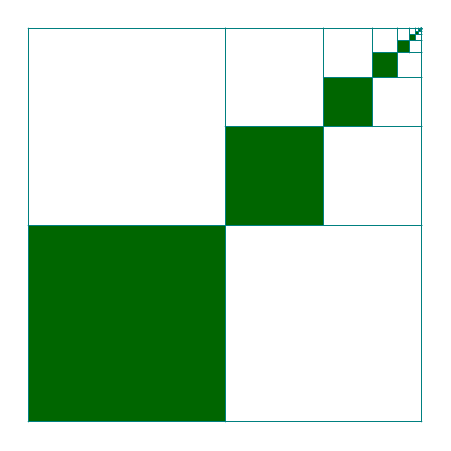
\begin{tikzpicture}[font=\footnotesize,line join=round,line cap=round,>=stealth,teal]
			\def\m{8} 
			\def\a{5} 
			\tikzset{hv/.pic={ 
			\fill[green!40!black](0,0)  rectangle (0.5*\a,0.5*\a);
			 \draw[step=0.5*\a](0,0) grid (\a,\a);
				}} 
			 \def\l{0}
			\foreach \i in {0,...,\m}{ 
				\pgfmathsetmacro{\n}{\l-(0.5)^\i*sqrt (2)*\a} 
				\path (45:\n) pic[scale={(0.5)^\i}]{hv}; 
				\global \let  \n = \l;
			 }
		\end{tikzpicture}
	} 
	 \choice
		{$6$} 
		 {$3$}
		{\True $5$} 
		{$4$} 
	 \loigiai{
		Diện tích của hình vuông lập thành cấp số nhân với số hạng đầu tiên  là $u_1=\dfrac{1}{4}$, $q=\dfrac{1}{4}\cdot$\\
		 Do đó số hạng tổng quát là $u_n=\dfrac{1}{4}\cdot \left(\dfrac{1}{4} \right)^{n-1}=\dfrac{1}{4^n}\; \left(n\ge 1\right)$.\\
		Để diện tích của hình vuông tô màu nhỏ  hơn $\dfrac{1}{1000} \Leftrightarrow \dfrac{1}{4^n} < \dfrac{1}{1000} \Leftrightarrow 4^n > 1000\Rightarrow n\ge 5$.\\
		Vậy tô  màu từ hình vuông thứ $5$ thỏa mãn yêu cầu bài toán.
	} 
\end{ex}

% nguồn: Ok_Toan11_TracNghiem_Lan2
\begin{ex}%[1D2V3-8]%[ma:054d9e34]
	Người  ta thiết kế một cái tháp $11$ tầng. Diện tích bề mặt trên của mỗi tầng bằng nửa diện tích của mặt trên của tầng ngay bên dưới và diện tích mặt trên của tầng $1$ bằng nửa diện tích của đế tháp. Tính diện tích mặt trên cùng, biết diện tích mặt trên của đế tháp là $12\,288$ m$^2$.
	\choice 
		 {$8$ m$^2$}
		{\True $6$ m$^2$} 
		{$10$  m$^2$}
		{$12$ m$^2$} 
	\loigiai{Gọi $a_0$, $a_1$, $a_2$, \dots, $a_{11}$ lần lượt là diện tích mặt trên của đế  tháp, tầng $1$, tầng $2$, \ldots, tầng $11$.\\
		Khi đó ta có $a_0  = 12\,288$; $a_n = \dfrac{1}{2} a_{n-1} = a_0 \left(\dfrac{1}{2} \right)^n$, $n = 1$, $2$, \dots, $11$.\\
	Diện tích mặt trên tầng trên cùng  là $a_{11} = a_0 \left(\dfrac{1}{2} \right)^{11} = 12\,288 \left(\dfrac{1}{2} \right)^{11} = 6$ m$^2$.}
\end{ex}

% nguồn: Ok_Toan11_TracNghiem_Lan2
\begin{ex}%[1D2C3-8]%[ma:4367c04b]
	Tam giác mà ba đỉnh của nó là ba trung điểm ba cạnh của tam giác $ABC$ được gọi là tam giác trung bình của tam giác $ABC$. Ta xây dựng dãy các tam giác $A_1B_1C_1, {\rm \;}A_2B_2C_2, {\rm \;}A_3B_3C_3, \ldots$ sao cho $A_1B_1C_1$ là một tam giác đều cạnh bằng $3$ và với mỗi  số nguyên dương $n\ge 2$ tam giác $A_n B_n C_n$ là tam giác trung bình của tam giác $A_{n-1} B_{n-1} C_{n-1}$. Với mỗi số nguyên dương $n$ kí hiệu $S_n$ tương ứng là diện tích hình tròn ngoại tiếp tam giác $A_n B_n C_n$. Tính tổng $S=S_1+S_2+\cdots+S_n+\cdots$?
	\choice 
		{$S=\dfrac{15\pi}{4}$} 
		{\True$S=4\pi$} 
		 {$S=\dfrac{9\pi}{2}$}
		 {$S=5\pi$}
	\loigiai{Vì dãy các  tam giác $A_1B_1C_1, {\rm \;}A_2B_2C_2, {\rm \;}A_3B_3C_3, \ldots$ là các tam giác đều nên bán kính đường tròn ngoại tiếp các tam giác bằng cạnh $\times \dfrac{\sqrt{3}}{3}$.
		\begin{itemize}
			\item Với $n=1$  thì tam giác đều $A_1B_1C_1$ có cạnh bằng $3$ nên đường tròn ngoại tiếp tam giác $A_1B_1C_1$ có bán kính $R_1=3\cdot \dfrac{\sqrt{3}}{3}
			\Rightarrow S_1=\pi \left(3\cdot \dfrac{\sqrt{3}}{3} \right)^2$. 
			\item Với $n=2$ thì tam giác đều $A_2B_2C_2$ có cạnh bằng $\dfrac{3}{2}$ nên đường tròn ngoại tiếp tam giác  $A_2B_2C_2$ có bán kính $R_2=3\cdot \dfrac{1}{2}\cdot \dfrac{\sqrt{3}}{3}
			\Rightarrow S_2=\pi \left(3\cdot  \dfrac{1}{2}\cdot \dfrac{\sqrt{3}}{3} \right)^2$.
			\item Với $n=3$ thì tam  giác đều $A_3B_3C_3$ có cạnh bằng $\dfrac{3}{4}$ nên đường tròn ngoại tiếp tam giác $A_2B_2C_2$ có bán kính $R_3=3\cdot \dfrac{1}{4}\cdot \dfrac{\sqrt{3}}{3}
			\Rightarrow  S_3=\pi \left(3\cdot \dfrac{1}{4}\cdot \dfrac{\sqrt{3}}{3} \right)^2$.
		\end{itemize}
		Như vậy tam giác đều  $A_n B_n C_n$ có cạnh bằng $3\cdot \left(\dfrac{1}{2} \right)^{n-1}$ nên đường tròn ngoại tiếp tam giác $A_n B_n C_n$ có bán kính $R_n=3\cdot \left(\dfrac{1}{2} \right)^{n-1}\cdot \dfrac{\sqrt{3}}{3}
		\Rightarrow S_n=\pi \left(3\cdot \left(\dfrac{1}{2} \right)^{n-1}\cdot \dfrac{\sqrt{3}}{3} \right)^2$.\\ 
		Khi đó ta được dãy $S_1,  S_2, \ldots S_n\ldots$ là một cấp số nhân lùi vô hạn với số hạng đầu $u_1=S_1=3\pi$ và công bội $q=\dfrac{1}{4}$.\\
		Do  đó tổng $S=S_1+S_2+\cdots+S_n+\cdots=\dfrac{u_1}{1-q}=4\pi$.
	 }
\end{ex}


%%%%%%%%%%%%%%%% ĐÚNG/SAI %%%%%%%%%%%%%%%%

% nguồn: Ok_dungsai_lop11_Lan2
\begin{ex}%[1D2H3-8]%[ma:2c8b6671]
	Aladin nhặt được cây đèn thần, chàng miết tay vào cây đèn và gọi Thần đèn ra. Thần đèn cho chàng $3$ điều ước. Aladin ước $2$ điều đầu tiên tùy thích, nhưng điều ước thứ $3$ của chàng là: \, \lq\lq Ước gì ngày mai tôi lại  nhặt được cây đèn và Thần cho tôi số điều ước gấp đôi số điều ước ngày hôm nay\rq\rq. Thần đèn chấp thuận và mỗi ngày Aladin đều thực hiện theo quy tắc như trên: ước hết các điều đầu tiên và luôn chừa lại điều ước cuối cùng để kéo dài thỏa thuận với thần đèn cho ngày hôm sau. Khi đó
	\choiceTF 
		 {\True Ngày thứ hai Aladin ước $6$ điều}
		{\True Ngày thứ ba  Aladin ước $12$ điều}
		{Ngày thứ tư Aladin  ước $48$ điều}
		{Sau $10$ ngày  gặp Thần đèn, Aladin ước tất cả $3\,269$ điều ước}
	\loigiai{ 
		\begin{itemchoice}
			 \itemch \textbf{Đúng.} \\
			Ngày thứ nhất  Aladin ước $3$ điều.
			Ngày  thứ hai Aladin ước $2\cdot 3$ điều.
			\itemch  \textbf{Đúng.} \\
			Ngày thứ ba  Aladin ước $2\cdot 2\cdot 3=12$ điều.
			\itemch \textbf{Sai.}  \\
			 Ngày thứ tư Aladin ước $2\cdot 2^2\cdot 3=2^3\cdot 3$ điều.
			\itemch  \textbf{Sai.} \\
			Ngày thứ $10$  Aladin ước $2^9\cdot 3$ điều.\\
			Vậy sau $10$ ngày Aladin đã ước $3\left(1+2+2^2+2^3+\cdots+2^9\right)=3\left(\dfrac{1-2^{10}}{1-2} \right)=3\,069$  điều.
		\end{itemchoice}
	} 
\end{ex}

% nguồn: Ok_dungsai_lop11_Lan2
\begin{ex}%[1D2H3-8]%[ma:67cd0823]
	Trong một hồ sen, số lá sen ngày hôm sau bằng $3$ lần số lá sen ngày hôm trước. Biết  rằng ngày đầu có $1$ lá sen thì tới ngày thứ $10$ hồ sẽ đầy lá sen.
	 \choiceTF
		{\True Nếu ngày đầu  có $9$ lá sen thì tới ngày thứ $8$ hồ sẽ đầy lá sen}
		{\True Số lá sen lập thành cấp số nhân $\left(u_n \right)$ với $u_1=1$ và công bội $q=3$} 
		{Số lá sen lập thành cấp số cộng $\left(u_n \right)$ với $u_1=1$  và công bội $q=3$}
		{Nếu ngày đầu có $9$ lá sen thì tới ngày thứ  $9$ hồ sẽ đầy lá sen}
	 \loigiai{
		Ngày đầu có có $u_1=1$  lá sen.
		Do số lá sen ngày  hôm sau bằng $3$ lần số lá sen ngày hôm trước nên ta có cấp số nhân $\left(u_n \right)$ với $u_1=1$ và công bội $q=3$.\\
		Vì  ngày thứ $10$ hồ sẽ đầy lá sen nên có $u_{10}=u_1\cdot q^9=1\cdot 3^9=3^9$ lá sen.\\
		Ngày đầu có $v_1=9$ lá  sen.\\
		Do số lá sen ngày hôm sau bằng $3$ lần số lá sen ngày hôm trước nên ta có cấp số  nhân $\left(v_m \right)$ với $v_1=9$ và công bội $q=3$.\\
		Khi đó sau $m$ ngày thì số lá sen là $v_m=v_1\cdot q^{m-1}=9\cdot  3^{m-1}$.\\
		Ta có $9\cdot  3^{m-1}=3^9\Leftrightarrow 3^{m+1}=3^9\Leftrightarrow m+1=9\Leftrightarrow m=8$.
		\begin{itemchoice}
			 \itemch \textbf{Đúng.}
			\itemch  \textbf{Đúng.}
			 \itemch \textbf{Sai.}
			\itemch  \textbf{Sai.}
		\end{itemchoice}
	} 
\end{ex}

% nguồn: Ok_dungsai_lop11_Lan1
\begin{ex}%[1D2V3-8]%[ma:f1c8a8a1]
 Người ta thiết kế  một cái tháp gồm $11$ tầng. Diện tích bề mặt sàn của mỗi tầng bằng $\dfrac{4}{5}$ diện tích của mặt sàn của tầng ngay bên dưới và diện tích mặt sàn của tầng $1$ bằng $\dfrac{4}{5}$ diện tích của đế tháp (đế tháp có diện tích là $75$ m$^2$). Tiền công thuê thợ xây cho bởi bảng sau:
 \begin{center}
  \begin{tabular}{|c|c|c|c|c|}
   \hline 
   & Đế tháp &Tầng $1$ đến tầng $5$ &Tầng  $6$ đến tầng $10$ & Tầng $11$ \\
    \hline
   Giá tiền trên $1$ m$^2$ (nghìn đồng) & 1000 & 850 & 900 &950 \\ 
    \hline
  \end{tabular}
 \end{center}
 \choiceTF 
  {\True  Tiền công xây tầng $1$ là $51$ triệu}
   {Tiền công xây tầng $11$ (làm tròn đến hàng nghìn) là $7650000$ đồng}
  {\True Tổng tiền công  xây tòa tháp (làm tròn đến hàng nghìn) là $312044000$ đồng}
  {Diện tích mặt sàn tầng $2$ là  $60$ m$^2$}
 \loigiai{ 
  Gọi $u_1$, $u_2$, $\ldots$, $u_{11}$ lần lượt là diện tích mặt sàn của tầng $1$, $2$, $\ldots$, $11$. 
  \begin{itemchoice}
   \itemch Theo giả thiết ta có, diện  tích mặt sàn tầng $1$ là $u_1=\dfrac{4}{5}\cdot 75=60$ (m$^2$).\\
   Vì diện tích mỗi mặt sàn bằng $\dfrac{4}{5}$ diện tích mặt sàn tầng ngay bên dưới nên dãy $u_1$,  $u_2$, $\ldots$, $u_{11}$ lập thành một cấp số nhân hữu hạn với số hạng đầu $u_1=60$, công bội $q=\dfrac{4}{5}$.\\
   Tiền công xây tầng $1$ là $60\cdot  850=51 \times 10^6= 51$ (triệu đồng).
   \itemch Giá trị $u_{11}=u_1\cdot \left(\dfrac{4}{5}\right)^{10}=48$  (m$^2$).
   Số tiền  xây là $48\times 950=45600000$ đồng.
   \itemch Số tiền  xây đế tháp là $75$ triệu đồng.\\
   Số  tiền xây tầng $1$ đến tầng $5$ là $(u_1+u_2+u_3+u_4+u_5)\cdot 850=u_1\cdot \dfrac{1-q^5}{1-q}\cdot 850=60\cdot \dfrac{1-\left(\tfrac{4}{5}\right)^5}{1-\tfrac{4}{5}}\cdot 850\quad (\text{nghìn đồng}).$\\
    Số tiền xây từ tầng $6$ đến tầng $10$ là
   $(u_6+u_7+u_8+u_9+u_{10})\cdot 950=u_1\cdot q^5\cdot \dfrac{1-q^5}{1-q}\cdot 900.$\\ 
   Tổng  tiền xây dựng tòa tháp là
   $75.000+60\cdot \dfrac{1-\left(\tfrac{4}{5}\right)^5}{1-\tfrac{4}{5}}\cdot 850+u_1\cdot q^5\cdot \dfrac{1-q^5}{1-q}\cdot 900 =312044000\quad (\text{nghìn đồng}).$ 
   \itemch Diện tích mặt sàn tầng  hai là $u_2=u_1\cdot q=60\cdot \dfrac{4}{5}=48$ (m$^2$).
 \end{itemchoice}}
\end{ex}

% nguồn: Ok_dungsai_lop11_Lan2
\begin{ex}%[1D2V3-8]%[ma:297f68d7]
	Để tích lũy cho việc học đại học của cậu con trai đầu lòng, cô Lan quyết định hằng tháng bỏ ra $600$ nghìn đồng vào  tài khoản tiết kiệm, được trả lãi $0,5\%$ cộng dồn hằng tháng. Cô bắt đầu chương trình tích lũy này khi cậu con trai tròn ba tuổi và gửi tiền vào đầu mỗi tháng. Xét tính đúng sai của các khẳng định sau:
	 \choiceTF
		{Số tiền mà cô Lan có trong chương trình tích lũy ở đầu tháng  thứ hai là $1\,200\,000$ triệu đồng}
		{Số tiền của cô Lan có  trong chương trình ở đầu tháng thứ $n$ là $ \dfrac{6\cdot 1{,}5^n-6}{5}$ (triệu đồng)}
		{\True Số tiền của cô Lan có trong chương trình ở đầu tháng thứ 5 (làm tròn đến hàng nghìn)  là $3\,030\,000$ đồng}
		{Số tiền  của cô Lan có trong chương trình vào thời điểm cậu con trai đầu lòng tròn $18$ tuổi nhỏ hơn $160$ triệu đồng}
	 \loigiai{
		\begin{itemchoice}
			\itemch 
			Gọi $u_n$ là số triệu đồng mà cô Lan có trong chương trình tích lũy ở lần gửi thứ $n$ (vào đầu tháng thứ $n$). Kí hiệu $a=0{,}6$  triệu đồng, $r=0{,}5\%$.\\
			Số tiền của cô Lan có trong chương trình ở đầu tháng  thứ nhất là $u_1=a$.\\
			Số tiền của cô Lan có trong chương trình ở đầu tháng thứ $2$ là $u_2=a(1+r) +a=0{,}6(1+0{,}5\%)  +0{,}6=1{,}203$ (triệu đồng).
			 \itemch
			Số tiền của cô Lan có trong chương trình ở đầu tháng thứ $3$  là $u_3=a(1+r)^2+a(1+r) +a$.\\
			Tương tự cho các tháng tiếp theo, suy ra số tiền của cô Lan có trong chương trình  ở đầu tháng thứ $n$ là
			\begin{align*}
				u_n&=a(1+r)^{n-1}+a(1+r)^{n-2}+...+a(1+r)  +a\\
				&=a.\dfrac{(1+r)^n-1}{(1+r)  -1}\\
				&=a\cdot \dfrac{(1+r)^n-1}{r}\\ 
				&=0,6\cdot  \dfrac{(1+0{,}5\%)^n-1}{0{,}5}\\
				&=\dfrac{6\cdot 1{,}005^n-6}{5}. 
			\end{align*}
			\itemch  Số tiền của cô Lan có trong chương trình ở đầu tháng thứ $5$ là
			 \[u_5=a.\dfrac{(1+r)^5-1}{r}=0{,}6.\dfrac{(1+0{,}5\%)^5-1}{0{,}5\%}=3{,}03~(\text{triệu đồng)}.\]
			\itemch Vào thời điểm cậu con trai đầu lòng tròn $18$ tuổi là thời điểm gửi khoản tiền thứ  $180$. Lúc đó cô sẽ tích lũy được \[u_{180}=a\dfrac{(1+r)^{180}-1}{r}=0{,}6\dfrac{(1+0{,}5\%)^{180}-1}{0{,}5\%}\approx 174{,}49~(\text{triệu đồng})\].
		\end{itemchoice}
	} 
\end{ex}

% nguồn: Ok_dungsai_lop11_Lan2
\begin{ex}%[1D2V3-8]%[ma:bfe46079]
	Aladin nhặt được cây đèn thần, chàng miết tay vào cây đèn và gọi Thần đèn ra. Thần đèn cho chàng $3$ điều ước. Aladin ước $2$ điều đầu tiên tùy thích, nhưng điều ước thứ $3$ của chàng là \lq\lq Ước gì ngày mai tôi lại nhặt được cây đèn và Thần cho tôi số điều ước gấp đôi số điều ước ngày hôm nay\rq\rq. Thần đèn  chấp thuận và mỗi ngày Aladin đều thực hiện theo quy tắc như trên$\colon$ ước hết các điều đầu tiên và luôn chừa lại điều ước cuối cùng để kéo dài thỏa thuận với Thần đèn cho ngày hôm sau.
	Xét tính đúng sai của các khẳng định sau 
	\choiceTF 
		 {\True Ngày thứ hai Aladin ước $6$ điều}
		{\True Ngày thứ ba Aladin ước $12$ điều} 
		{Ngày thứ tư Aladin ước $48$  điều}
		{Sau $10$ ngày gặp Thần đèn, Aladin ước  tất cả $3269$ điều ước}
	 \loigiai{
		\begin{itemchoice}
			\itemch 
			Ngày đầu tiên  Aladin ước $3$.\\
			Ngày thứ hai $2 \cdot  3 = 6$.
			\itemch 
			Ngày thứ ba $2 \cdot 2 \cdot 3 = 2^2  \cdot 3 = 12$.
			 \itemch
			Ngày thứ tư $2 \cdot 2^2 \cdot 3 = 2^3 \cdot  3 = 24$.
			\itemch 
			Tổng số điều  ước sau $10$ ngày là
			 \[
			3\cdot \left(1 + 2 + 2^2 + \ldots + 2^9\right) = 3\cdot \left(\frac{1 - 2^{10}}{1 - 2}\right) = 3 \cdot (2^{10} - 1) = 3  \cdot 1023 = 3069\neq 3269.
			\] 
		\end{itemchoice}
	} 
\end{ex}

% nguồn: Ok_dungsai_lop11_Lan2
\begin{ex}%[1D2V3-8]%[ma:e14b5edb]
	Tương truyền rằng nhà vua Ấn Độ cho phép người phát minh ra bàn cờ vua được lựa chọn phần thưởng tùy theo sở thích. Người đó xin nhà vua: \lq\lq Bàn cờ có $64$ ô, với ô thứ nhất thần xin nhận $1$ hạt thóc, ô thứ hai thì gấp đôi ô đầu, ô thứ ba thì lại gấp đôi ô thứ hai,... cứ như vậy ô sau nhận số hạt thóc gấp đôi phần thưởng dành cho ô liền trước và thần xin nhận tổng số các hạt thóc ở $64$ ô. Biết rằng khối lượng  của $100$ hạt thóc là $20$ gam.
	\choiceTF 
		{\True Số hạt thóc ở $64$ ô là một cấp số nhân có $u_1=1$; $q=2$} 
		{Số hạt thóc ở ô thứ tám  là $2^8$}
		{Tổng khối lượng thóc của $64$  ô trên bàn cờ là $364$ tỉ tấn}
		{Giả sử người đó muốn chở  số thóc ở trên $32$ ô đầu tiên về bằng tàu thủy, biết rằng mối chuyến tàu chở tối đa $10$ tấn hàng hóa. Khi đó, người đó cần tối thiểu $85$ chuyến tàu để chở hết số thóc đó}
	 \loigiai{
		\begin{itemchoice}
			\itemch \textbf{Đúng} \\ 
			Số hạt thóc ở $64$ ô là môt cấp  số nhân có $u_1=1$; $q=2$.
			\itemch \textbf{Sai} \\ 
			Số hạt  thóc ở ô thứ tám là $u_{8}=u_1\cdot q^7=2^7$.
			\itemch \textbf{Sai}  \\
			Tổng số  hạt thóc của $64$ ô là $S_{64}=1+2+2^2+\ldots+2^{63}=2^{64}-1$ hạt thóc.\\
			Do đó, tổng khối lượng thóc trên $64$ ô trên bàn cờ là  \[\left(2^{64}-1\right) \cdot \dfrac{20}{100} \approx 3.69 \cdot 10^8\text{ (g)}=369 \text{ (tỉ tấn)}.\]
			\itemch  \textbf{Sai} \\
			Kkhối lượng thóc của $32$ ô đầu tiên là $\left(2^{32}-1\right) \cdot \dfrac{20}{100}=858\,993\,459 \approx  859$ (tấn).\\
			 Mỗi tàu chở tối đa $10$ tấn hàng hóa thì cần tối thiểu $86$ chuyến tàu để có thể chở hết số thóc trên.
		\end{itemchoice}
	} 
\end{ex}

% nguồn: Ok_dungsai_lop11_Lan2
\begin{ex}%[1D2V3-8]%[ma:737bd47c]
	Để tích lũy cho việc học đại học của cậu con trai đầu lòng, cô Lan quyết định hằng tháng bỏ ra $600$ nghìn đồng vào tài khoản tiết kiệm, được trả lãi $0{,}5\%$ cộng dồn hằng tháng. Cô bắt đầu chương trình tích lũy  này khi cậu con trai tròn ba tuổi và gửi tiền vào đầu mỗi tháng.
	 \choiceTF
		{Đến lần gửi khoản tiền thứ $180$ thì cậu  con trai tròn $18$ tuổi}
		{Số tiền của  cô Lan có trong chương trình ở đầu tháng thứ $2$ là $0{,}6\left(1+0{,}5\% \right)$ triệu đồng}
		{Số tiền của cô Lan có trong chương trình  ở đầu tháng thứ $5$ (làm tròn đến hàng nghìn) là $3\,030\,000$ đồng}
		{Số tiền của cô Lan có trong chương trình vào thời điểm  cậu con trai đầu lòng tròn $18$ tuổi nhỏ hơn $160$ triệu đồng}
	 \loigiai{
		Gọi $u_n$ là số triệu đồng mà cô Lan có trong chương trình tích lũy ở lần gửi thứ $n$ (vào đầu tháng thứ $n$). Kí hiệu $a=0{,}6$ triệu đồng, $r=0{,}5\%$. 
		Số tiền  của cô Lan có trong chương trình ở đầu tháng thứ nhất là $u_1=a$.
		Số tiền của cô Lan có trong chương trình  ở đầu tháng thứ $2$ là
		\[u_2=a\left(1+r\right)+a=0{,}6\left(1+0{,}5\% \right)+0{,}6. 
		\] 
		Số tiền của cô Lan có trong chương trình ở  đầu tháng thứ $3$ là $u_3=a\left(1+r\right)^2+a\left(1+r\right)+a$.
		Tương tự cho các tháng tiếp theo, suy ra số tiền của cô Lan có trong chương trình ở đầu tháng thứ  $n$ là
		 \[u_n=a\left(1+r\right)^{n-1}+a\left(1+r\right)^{n-2}+\cdots+a\left(1+r\right)+a=a \cdot\dfrac{\left(1+r\right)^n-1}{\left(1+r\right)-1}=a\cdot\dfrac{\left(1+r\right)^n-1}{r}.
		 \]
		Số tiền của cô Lan có trong chương trình  ở đầu tháng thứ $5$ là\\
		$u_5=a\cdot\dfrac{\left(1+r\right)^5-1}{r}=0{,}6\cdot\dfrac{\left(1+0{,}5\% \right)^5-1}{0{,}5\%} \approx 3{,}03$ triệu đồng $=3\,030\,000$  đồng.\\
		Vào thời điểm cậu con trai đầu lòng tròn $18$ tuổi là  thời điểm gửi khoản tiền thứ $180$.
		Lúc đó cô  sẽ tích lũy được $u_{180}=a\cdot\dfrac{\left(1+r\right)^{180}-1}{r}=0{,}6\cdot\dfrac{\left(1+0{,}5\% \right)^{180}-1}{0{,}5\%} \approx 174{,}49$ (triệu đồng).
		\begin{itemchoice}
			\itemch \textbf{Đúng.} 
			\itemch \textbf{Sai.} 
			 \itemch \textbf{Đúng.}
			\itemch \textbf{Sai.} 
		\end{itemchoice}
	} 
\end{ex}

% nguồn: Ok_dungsai_lop11_Lan2
\begin{ex}%[1D2V3-8]%[ma:c87d6c2a]
	Tương truyền rằng nhà vua Ấn Độ cho phép người phát minh ra bàn cờ vua được lựa chọn phần thưởng tùy theo sở thích. Người đó xin nhà vua $1$ Bàn cờ có $64$ ô, với ô thứ nhất thần xin nhận $1$ hạt thóc, ô thứ hai thì gấp đôi ô đầu, ô thứ  ba thì lại gấp đôi ô thứ hai, \ldots, cứ như vậy ô sau nhận phần thưởng dành cho ô liền trước và thần xin nhận tổng số các hạt thóc ở $64$ ô\rq\rq. Biết rằng khối lượng của $100$ hạt thóc là $20$ gam.
	\choiceTF 
		{\True Số hạt thóc ở $64$ ô là  một cấp số nhân có $u_1=1$; $q=2$}
		{Số hạt  thóc ở thứ tám là $2^8$}
		{Tổng khối lượng thóc của $64$ ô trên  bàn cờ là $364$ tỉ tấn}
		{Giả sử người đó muốn chở số thóc ở trên $32$ ô đầu tiên về bằng tàu thủy, biết rằng mỗi chuyến tàu chở tối đa $10$ tấn hàng hóa. Khi đó,  người đó cần tối thiểu $85$ chuyến tàu để chở hết số thóc đó}
	\loigiai{Số hạt thọc ở $64$ ô là một cấp số nhân có  $u_1=1$; $q=2$. \\
		Khi đó số hạt thóc ở ô thứ $8$ là $u_8=u_1q^{7}=2^7$.\\ 
		Tổng  số hạt thóc của $64$ ô là $S_{64}=1+2^1+2^2+\ldots+2^{63}=2^{64}-1$ hạt thóc. \\
		Do đó tổng khối lượng thóc trên $64$ ô trên bàn cờ là $\left(2^{64}-1 \right)\cdot \dfrac{20}{100} \approx 3{,}69 \times 10^{18} \ \text{(g)}  =369$ (tỉ tấn).\\
		Tương tự, ta  có khối lượng thóc của $32$ ô đầu tiên là $\left(2^{32}-1 \right)\cdot \dfrac{20}{100}=858\,993\,459 \approx 859$ (tấn).
		\begin{itemchoice}
			\itemch Số hạt thóc ở $64$ ô là một cấp số nhân có $u_1=1$;  $q=2$.
			\itemch Số hạt thóc ở ô thứ tám là  $2^7$.
			\itemch Tổng khối lượng thóc của $64$ ô trên bàn cờ là  $369$ tỉ tấn.
			 \itemch
		\end{itemchoice}
	 }
\end{ex}

% nguồn: Ok_dungsai_lop11_Lan2
\begin{ex}%[1D2V3-8]%[ma:f36d1acb]
	Ông An bắt đầu  đi làm với mức lương khởi điểm là $5\,000\,000$ đồng một tháng. Cứ sau một chu kỳ $3$ năm thì ông An được tăng lương $4\%$. Xét tính đúng sai của các khẳng định sau:
	\choiceTF 
		{\True Mức lương ông An nhận được sau  $3$ năm là $5\,200\,000$ đồng}
		{Tổng  số tiền lương ông An nhận được sau $6$ năm đầu là $374\,400\,000$ đồng}
		{Dự đoán công thức tính số tiền lương ông An được nhận $u_n$, sau $n$ chu kì năm công tác là $u_n=5\,000\,000\cdot\left(\dfrac{26}{25}\right)^n$ đồng} 
		{\True Giả sử ông  An đi làm sau đúng $35$ năm thì được về hưu. Tổng số tiền lương ông nhận được trong cả quá trình công tác là $2\,612\,277\,740$ đồng}
	\loigiai{ 
		\begin{itemchoice}
			\itemch Mức lương $3$ năm tiếp theo  của ông An là
			 \[
			5\,000\,000+5\,000\,000 \cdot  \dfrac{4}{100}=5\,000\,000 \cdot\left(1+\dfrac{1}{25}\right)=5\,200\,000 \text{ (đồng).}
			\] 
			 \itemch $1$ năm=$12$ tháng.\\
			Tổng lương $3$ năm đầu là $36\cdot5\,000\,000=180\,000\,000$  (đồng).\\
			Tổng lương từ năm thứ $4$ đến năm  thứ $6$ là $36\cdot5\,200\,000=187\,200\,000$ (đồng).\\
			Tổng số tiền lương ông An nhận được sau $6$ năm đầu là $$180\,000\,000+187\,200\,000=367\,200\,000  \, \text{ (đồng)}.$$
			\itemch Chu kì thứ nhất  mức lương của ông An là $u_1=5\,000\,000$ (đồng).\\
			Chu kì thứ hai mức lương của ông  An là
			\begin{eqnarray*}
				 u_2&=&5\,000\,000+5\,000\,000\cdot \dfrac{4}{100}\\
				&=&5\,000\,000\cdot\left(1+\dfrac{1}{25}\right)\\ 
				&=&5\,000\,000\cdot \dfrac{26}{25}\, \text{  (đồng).}
			\end{eqnarray*}
			Chu kì thứ ba mức lương của  ông An là
			\begin{eqnarray*}
				u_3&=&5\,000\,000\cdot\left(\dfrac{26}{25}\right)+5\,000\,000\cdot\left(\dfrac{26}{25}\right)  \cdot \dfrac{1}{25}\\
				 &=&5\,000\,000\cdot\left(\dfrac{26}{25}\right) \cdot\left(1+\dfrac{1}{25}\right)\\
				 &=&5\,000\,000\cdot\left(\dfrac{26}{25}\right)^2\,\text{ (đồng).}
			\end{eqnarray*}
			Chu kì  thứ tư mức lương của ông An là
			\begin{eqnarray*}
				u_4&=&5\,000\,000\cdot\left(\dfrac{26}{25}\right)^2+5\,000\,000\cdot\left(\dfrac{26}{25}\right)^2\cdot \dfrac{1}{25}\\ 
				&=&5\,000\,000\cdot\left(\dfrac{26}{25}\right)^2\left(1+\dfrac{1}{25}\right)\\ 
				&=&5\,000\,000\cdot\left(\dfrac{26}{25}\right)^3\,\text{ (đồng).} 
			\end{eqnarray*}
			Cứ tiếp tục như vậy ta dự đoán được sau chu kì thứ $n$ số tiền lương  ông An nhận được là
			 $$ u_n=5\,000\,000\cdot\left(\dfrac{26}{25}\right)^{n-1} \,\text{ (đồng).}$$
			\itemch Tổng tiền lương của chu kì thứ nhất  là $36\cdot5\,000\,000=180\,000\,000$ (đồng).\\
			Tổng tiền lương của chu kì thứ hai là $36\cdot5\,000\,000\cdot \dfrac{26}{25}$ (đồng).\\ 
			Tổng tiền lương  của chu kì thứ ba là $36\cdot5\,000\,000\cdot\left(\dfrac{26}{25}\right)^2$ (đồng).\\
			Tổng tiền lương của chu kì thứ mười một là $36\cdot5\,000\,000\cdot\left(\dfrac{26}{25}\right)^{10}$  (đồng).\\
			Tổng tiền lương $2$ năm tiếp theo  của chu kì thứ mười hai là $24\cdot5\,000\,000\cdot\left(\dfrac{26}{25}\right)^{11}$ (đồng).\\
			Tổng tiền lương sau tròn $35$  năm là
			\begin{eqnarray*}
				 S&=&36\cdot5\,000\,000+36\cdot5\,000\,000 \cdot\left(\dfrac{26}{25}\right)+\cdots
				+36\cdot5\,000\,000  \cdot\left(\dfrac{26}{25}\right)^{10}+24\cdot5\,000\,000\cdot\left(\dfrac{26}{25}\right)^{11}\\
				&=&36\cdot5\,000\,000\left(1+\dfrac{26}{25}+\left(\dfrac{26}{25}\right)^2+\cdots+\left(\dfrac{26}{25}\right)^{10}\right)+24\cdot5\,000\,000\cdot\left(\dfrac{26}{25}\right)^{11} \\ 
				&=&\dfrac{36\cdot5\,000\,000  \cdot\left(1-\left(\dfrac{26}{25}\right)^{11}\right)}{1-\dfrac{26}{25}}+24\cdot5\,000\,000\cdot\left(\dfrac{26}{25}\right)^{11}\\
				&=&2\,612\,277\,740 \text{  (đồng).}
			\end{eqnarray*}
		\end{itemchoice}
	} 
\end{ex}

% nguồn: Ok_dungsai_lop11_Lan2
\begin{ex}%[1D2V3-8]%[ma:ef769680]
	Vào năm con gái được $4$ tuổi, một người chuẩn bị gửi tiết kiệm đều mỗi năm một số tiền $x$ (triệu đồng) ($x \in \mathbb{N}$) để đến năm $18$ tuổi sẽ có được  $200$ triệu cho con gái đi học đại học. Hiện tại lãi suất tiền gửi hằng năm là $4{,}8\%$/năm. Giả sử lãi suất này được giữ ổn định. Xét tính đúng sai của các khẳng định sau:
	\choiceTF 
		{Tổng  số tiền thu về sau $14$ năm là một cấp số nhân có $q=(1+4{,}8\%)$}
		{Tổng  số tiền thu về sau $14$ năm là một cấp số nhân có $u_1 = x$}
		{\True $x =  10$ (triệu đồng)}
		{\True Đến năm con gái được $10$ tuổi, người này dự định khi con gái được $18$ tuổi sẽ mua thêm cho con gái một chiếc xe máy trị giá $50$ triệu đồng. Do đó, kể từ thời điểm đầu năm con gái được $10$ tuổi người này cần gửi tiết kiệm $y$ triệu đồng đến khi con gái  $18$ tuổi ($y \in \mathbb{N}$). Giá trị nhỏ nhất của $y$ là $15$}
	\loigiai{ 
		Số tiền người đó nhận được sau năm thứ nhất là: $A_1  = x(1+4{,}8\%)$.\\
		Số tiền người đó nhận được sau năm thứ hai là: $A_2  = x(1+4{,}8\%) + x(1+4{,}8\%)^2$.\\
		Số tiền người đó nhận được sau năm thứ $14$ là: $A_{14} = x(1+4{,}8\%) + x(1+4{,}8\%)^2 + \ldots + x(1+4{,}8\%)^{14}$.\\ 
		Khi đó  $A_{14}$ là tổng 14 số hạng đầu của cấp số nhân có $\heva{&u_1 = x(1+4{,}8\%)\\&q = (1+4{,}8\%).}$\\
		Suy ra  $A_{14} = u_1\dfrac{q^{n}-1}{q-1} = x(1+4{,}8\%) \cdot \dfrac{(1+4{,}8\%)^{14} -1}{4{,}8\%}$.\\
		Do  $A_{14}\ge 200$ nên
		 \[
		x \ge \dfrac{200 \cdot 4{,}8\%}{(1+4{,}8\%)\left[(1+4{,}8\%)^{14}-1\right]} \approx 9{,}873336. 
		 \]
		Do  $x\in \mathbb{N}$ nên $x = 10$ (triệu đồng).\\
		Gọi $z = y - x$ ($z\in \mathbb{N}$) là số tiền mà người đó phải gửi thêm mỗi năm kể từ năm con gái $10$ tuổi (năm thứ $6$) và $P_8 = z(1+4{,}8\%) + z(1+4{,}8\%)^2 + \ldots + z(1+4{,}8\%)^8$  là số tiền nhận được sau $8$ năm.\\
		Khi đó để nhận được số tiền $250$ triệu đồng vào năm con gái $18$ tuổi ($8$  năm kể từ con gái $10$ tuổi) thì:
		 \[
		P_8 = 250 -  10(1+4{,}8\%) \cdot \dfrac{(1+4{,}8\%)^{14}-1}{4{,}8\%} \approx 47{,}43 \text{ (triệu đồng)}.
		 \]
		 Suy ra
		\[ 
		z \ge \dfrac{47{,}43 \cdot 4{,}8\%}{(1+4{,}8\%)\left[(1+4{,}8\%)^8-1\right]} \approx 4{,}77. 
		 \]
		Vì $z\in \mathbb{N}$ nên $z=5$ (triệu đồng).\\ 
		Vậy $y = 15$  (triệu đồng).
		\begin{itemchoice}
			\itemch Tổng số tiền thu về sau $14$ năm là tổng của cấp số nhân có  $q = (1+4{,}8\%)$.
			 \itemch Tổng số tiền thu về sau $14$ năm là một cấp số nhân có $u_1 = x(1+4{,}8\%)$.
			\itemch $x =  10$ (triệu đồng).
			\itemch Đến năm con gái được $10$ tuổi, người này dự định khi con gái được $18$ tuổi sẽ mua thêm cho con gái một chiếc xe máy trị giá $50$ triệu đồng. Do đó, kể từ thời điểm đầu năm con gái được $10$ tuổi người này cần gửi tiết kiệm $y$ triệu đồng đến khi con gái $18$ tuổi ($y \in \mathbb{N}$). Giá trị nhỏ nhất  của $y=15$.
		\end{itemchoice}
	} 
\end{ex}

% nguồn: Ok_dungsai_lop11_Lan2
\begin{ex}%[1D2V3-8]%[ma:a79296f6]
	Trong một hồ sen, số lá sen ngày hôm sau bằng $3$  lần số lá sen ngày hôm trước. Biết rằng ngày đầu có $1$ lá sen thì tới ngày thứ $10$ hồ sẽ đầy lá sen. Xét tính đúng sai của các khẳng định sau
	\choiceTF 
		{\True Nếu ngày  đầu có $9$ lá sen thì tới ngày thứ $8$ hồ sẽ đầy lá sen}
		 {\True Số lá sen lập thành cấp số nhân($u_n$) với $u_1=1$ và công bội $q=3$}
		{Số lá sen lập thành cấp  số cộng($u_n$) với $u_1=1$ và công sai $d=3$}
		{Nếu ngày đầu có $9$ lá sen thì tới ngày thứ $9$ hồ sẽ đầy  lá sen}
	\loigiai{ 
		Ngày đầu có có $u_1 = 1$ lá sen. Do số lá sen ngày hôm sau bằng $3$ lần số lá sen ngày hôm trước nên ta có cấp số nhân($u_n$) với $u_1=1$ và công bội $q=3$. Vì ngày thứ $10$ hồ sẽ đầy lá sen nên có $u_{10}=u_1.q^9 = 1.3^9 = 3^9$ lá sen. Ngày đầu có $v_1 = 9$ lá sen. Do số lá sen ngày hôm sau bằng $3$  lần số lá sen ngày hôm trước nên ta có cấp số nhân($v_n$) với $v_1=9$ và công bội $q=3$. Khi đó sau $m$ ngày thì số lá sen là $v_m=v_1.q^{m-1} = 9.3^{m-1}$. Ta có $9.3^{m-1} = 3^9 \Leftrightarrow 3^2.3^{m-1} = 3^9 \Leftrightarrow 3^{m+1} = 3^9 \Leftrightarrow m+1=9 \Leftrightarrow m=8$.
		\begin{itemchoice}
			\itemch Nếu ngày đầu có $9$ lá sen thì tới ngày thứ $8$ hồ sẽ đầy lá sen. 
			\itemch Số lá sen lập thành cấp  số nhân($u_n$) với $u_1=1$ và công bội $q=3$.
			\itemch Số lá sen lập thành  cấp số nhân($u_n$) với $u_1=1$ và công bội $q=3$.
			\itemch Nếu ngày đầu có $9$ lá sen thì tới ngày thứ $8$ hồ  sẽ đầy lá sen.
		\end{itemchoice}
	 }
\end{ex}

% nguồn: Ok_dungsai_lop11_Lan2
\begin{ex}%[1D2V3-8]%[ma:9473f9b0]
	Anh Bình là nhân viên của một công ty A. Từ ngày $1$/$2$/$2024$ anh Bình được nâng lương lên bậc $4$, mức lương anh hiện hưởng là $11\,718\,750$ đồng mỗi tháng (chưa trừ thuế và bảo hiểm). Theo quy định của công ty, nếu không bị kỉ luật, không có khen thưởng đặc biệt thì cứ sau $3$ năm anh Bình sẽ được nâng một bậc lương, tăng thêm $25$\% so với bậc lương trước, tối đa là bậc $7$. Khi hết bậc $7$ sẽ chuyển sang vượt khung. Lương vượt khung năm sau cao hơn năm trước $1$\% và vẫn nhận hàng tháng. Lương bậc $1$ sẽ được tính sau khi hết đúng $1$ năm tập sự. Anh Bình là người  rất nghiêm túc, không vi phạm kỉ luật. Anh dự định sẽ làm việc $30$ năm ở công ty này rồi nghỉ hưu (làm tròn đến đồng).
	\choiceTF 
		 {Lương bậc $5$ của anh Bình sẽ là $14\,500\,000$ đồng}
		 {\True Lương bậc $1$ của anh Bình là $6\,000\,000$ đồng}
		{Lương bậc $7$ anh Bình là $23\,250\,000$ đồng} 
		{\True Tổng tiền lương anh Bình nhận được kể từ khi hết tập sự đến  khi nghỉ hưu là $5\,554\,357\,709$ đồng}
	 \loigiai{
		Gọi $u_n$ là  lương bậc $n$ của anh Bình hàng tháng.\\
		 Ta có $u_{n+1}=u_n+25\% u_n=u_n\cdot 1{,}25\,(n\le 7)$
		$u_n$  là cấp số nhân có công bội $q=1{,}25$.
		\begin{itemchoice}
			\itemch \textbf{Sai.} \\ 
			 Ta có $u_4=11\,718\,750$ nên $u_5=u_4 \cdot 1{,}25=14\,648\,437{,}5$ đồng.
			\itemch \textbf{Đúng.} \\ $u_4=u_1 \cdot q^3\Leftrightarrow u_1=\dfrac{u_4}{q^3}=6\,000\,000$  đồng.
			 \itemch \textbf{Sai.} \\
			$u_7=u_1^{} \cdot q^6=6\,000\,000\cdot 1{,}25^6=22\,888\,184$ đồng. 
			\itemch \textbf{Đúng.} \\ Khi vượt khung, lương mỗi khung \%, là cấp số nhân $v_n, \left(1\le n\le 8\right)$ có số hạng đầu là  $v_1=u_7+1\% u_7=1{,}01u_7$, công bội là $q'=1{,}01$.
			Anh Bình làm việc $30$ năm liên tục, trong đó $1$ năm tập sự, $21$ năm lương theo bậc, $8$ năm vượt khung. Mỗi bậc lương anh Bình nhận $36$ tháng,  lương vượt khung mỗi khung \% anh nhận $12$ tháng.\\
			Tổng lương anh Bình nhận được kể  từ khi hết tập sự đến khi nghỉ hưu là
			 \[S=36u_1\cdot\dfrac{q^7-1}{q-1}+12v_1 \dfrac{q'^8-1}{q'-1} =5\,554\,357\,709 \,\text{đồng}.\]
		\end{itemchoice}
	 }
\end{ex}

% nguồn: Ok_dungsai_lop11_Lan2
\begin{ex}%[1D2C3-8]%[ma:7289fe15]
	Vào năm con gái được $4$ tuổi, một người chuẩn bị gửi tiết kiệm đầu mỗi năm một số tiền $x$ (triệu đồng) $(x \in \mathbb{N})$ để đến năm $18$ tuổi sẽ có được $200$ triệu cho con gái  đi học đại học. Hiện tại lãi suất tiền gửi hàng năm là $4{,}8 \%$/năm. Giả sử lãi suất này được giữ ốn định.
	 \choiceTF
		{\True Tổng số tiền thu về sau $14$  năm là một cấp số nhân có $q=(1+4{,}8\%)$}
		{Tổng số tiền thu về sau $14$  năm là một cấp số nhân có $u_1=x$}
		{\True $x=10$ (triệu  đồng)}
		{\True Đến năm con gái được $10$ tuổi, người này dự định khi con gái được $18$ tuổi sẽ mua thêm cho con gái một chiếc xe máy trị giá $50$ triệu đồng. Do đó, kể từ thời điểm con gái được $10$ tuổi người này cần gửi tiết kiệm $y$ triệu đồng đến khi con gái $18$ tuổi. Giá  trị nhỏ nhất của $y=15$}
	 \loigiai{
		\begin{itemchoice}
			 \itemch \textbf{Đúng} \\
			Số tiền người đó nhận được sau năm thứ nhất là  $A_1=x(1+4{,}8 \%)$.\\
			Số tiền người đó nhận được sau năm thứ hai là  $A_2=x(1+4{,}8 \%)+x(1+4{,}8 \%)^2$.\\
			Số tiền người đó nhận được sau năm thứ $14$ là 
			 $A_{14}=x(1+4{,}8 \%)+x(1+4{,}8 \%)^2+\ldots+x(1+4{,}8 \%)^{14}$.\\
			Khi đó, $A_{14}$ có  $\heva{&u_1=x(1+4{,}8 \%) \\ &q=(1+4{,}8 \%).}$
			 \itemch \textbf{Sai} \\
			$A_{14}$ có $\heva{&u_1=x(1+4{,}8 \%) \\ &q=(1+4{,}8  \%).}$
			 \itemch \textbf{Đúng} \\
			Vì $A_{14}$ có $\heva{&u_1=x(1+4{,}8 \%) \\ &q=(1+4{,}8 \%)}$ nên $A_{14}=u_1 \dfrac{q^n-1}{q-1}=x(1+4{,}8 \%)  \dfrac{(1+4{,}8 \%)^{14}-1}{4{,}8 \%}$.\\
			Suy ra $x=\dfrac{200\cdot  4{,}8 \%}{(1+4{,}8 \%)\left[(1+4{,}8 \%)^{14}-1\right]} \approx 9{,}873\,336 \approx 10$ (triệu đồng).
			 \itemch \textbf{Đúng} \\
			Goi $z=y-x$ là số tiền mà người đó phải gửi thêm mỗi năm kể từ năm con gái $10$ tuổi (năm thứ $6$) và $P_8=z(1+4{,}8 \%)+z(1+4{,}8  \%)^2+\ldots+z(1+4{,}8 \%)^8$ là số tiền nhân được sau $8$ năm.\\
			Khi đó để nhận được số tiền $250$ triệu đồng vào năm con gái $18$ tuổi  ($8$ năm kể từ con gái $10$ tuổi) thì
			\[P_8=250-10(1+4{,}8  \%) \dfrac{(1+4{,}8 \%)^{14}-1}{4{,}8 \%} \approx 47{,}43 \text{ (triệu đồng)}.\]
			Suy ra $z=\dfrac{47{,}43\cdot  4{,}8 \%}{(1+4{,}8 \%)\left[(1+4{,}8 \%)^8-1\right]} \approx 4{,}77 \approx 5$ (triệu đồng).\\
			Vậy $y=15$  (triệu đồng).
		\end{itemchoice}
	 }
\end{ex}

% nguồn: Ok_dungsai_lop11_Lan1
\begin{ex}%[1D2K3-8]%[ma:477bb222]
 Hãy cho  biết tính đúng sai của mỗi mệnh đề dưới đây?
 \choiceTF 
  {Người ta thiết kế một cái tháp gồm 10 tầng. Diện tích bề  mặt trên của mỗi tầng bằng nửa diện tích mặt trên của tầng ngay bên dưới và diện tích bề mặt của tầng 1 bằng $ \dfrac{2}{3} $ diện tích đế tháp. Biết diện tích mặt đế tháp là $ 6144 m^2 $. Diện tích mặt trên cùng bằng $ 6$m$^2 $}
  {\True Bảo tàng Hà Nội được xây dựng gồm hai tầng hầm  và
  bốn tầng nổi. Bốn tầng nổi được  dùng để trưng bày rất nhiều
  những hiện vật có giá trị. Diện tích sàn tầng nổi thứ  nhất xấp xỉ $12000$ m$^2$. Biết rằng mỗi tầng nổi tiếp theo có diện tích bằng $\dfrac{4}{3}$ diện tích tầng nổi ngay dưới nó. Tổng diện tích mặt sàn
  (làm tròn đến hàng đơn vị) của bốn  tầng nổi dùng để trưng bày hiện vật của bảo tàng bằng $77778$ m$^2$}
  {\True Một hãng taxi X áp dụng mức giá đối với khách hàng theo hình thức bậc thang như sau: mỗi bậc áp dụng cho 10 km. Bậc 1 (áp dụng cho 10 km đầu) có giá 10.000 đồng $/$ 1 km, giá mỗi km ở các bậc tiếp theo giảm 5\% so với giá của bậc trước đó. Bạn Toàn thuê hãng taxi X đó để đi hết quãng đường 42  km. Số tiền (kết quả làm tròn đến hàng nghìn) mà bạn Toàn phải trả là $387000$ đồng}
  {Anh $A$ vào làm ở công ty $X$ với mức lương ban đầu $10$ triệu đồng/tháng. Nếu hoàn thành tốt nhiệm vụ thì cứ  sau $6$ tháng làm việc, mức lương của anh lại được tăng thêm $20\%$. Bắt đầu từ tháng thứ $24$ kể từ khi vào làm công ty $X$, tiền lương mỗi tháng của anh nhiều hơn $20$ triệu đồng? (biết rằng trong suốt thời gian làm ở công ty $X$ anh $A$ luôn hoàn thành tốt nhiệm vụ)}
 \loigiai{ 
  \begin{itemchoice}
   \itemch Gọi $ u_n $ là diện tích của tầng tháp thứ $ n $.\\ 
   Ta có $ (u_n) $ là cấp số nhân với $ u_1=\dfrac{2}{3}\cdot6144=4096 $ và $ q=\dfrac{1}{2}  $.\\
   Từ đó  diện tích mặt trên cùng (tầng thứ $10$) là $ u_{10}=u_1 \cdot q^{n-1}=4096 \cdot {\left( \dfrac{1}{2} \right)}^{9}=8$m$^2 $.
   \itemch Ta có diện tích sàn tầng nổi thứ nhất là $S_1=12000$ m$^2$.\\ 
   Suy ra diện  tích sàn tầng nổi thứ hai là $S_2=\dfrac{4}{3}S_1=\dfrac{4}{3}\cdot 12000=16000$ m$^2$.\\
   Diện tích sàn tầng nổi thứ ba là $S_3=\dfrac{4}{3}S_2=\dfrac{4}{3}\cdot 16000=\dfrac{64000}{3}$  m$^2$.\\
   Diện  tích sàn tầng nổi thứ tư là $S_4=\dfrac{4}{3}S_3=\dfrac{4}{3}\cdot \dfrac{64000}{3}=\dfrac{256000}{9}$ m$^2$.\\
   Vậy tổng diện  tích mặt sàn của bốn tầng nổi là $S_1+S_2+S_3+S_4\approx 77778$ m$^2$.
   \itemch Gọi $T_1$ là giá của mỗi km ở  bậc 1.\\
   $T_2$  là giá của mỗi km ở bậc 2.\\
   $T_3$ là giá của  mỗi km ở bậc 3.\\
   $T_4$ là giá  của mỗi km ở bậc 4.\\
   $T_5$ là giá của mỗi km ở bậc 5.\\ 
   Ta thấy, dãy $T_n (1 \le n \le 5)$ là một cấp số nhân, với  số hạng đầu $T_1=10000$ và công bội $q=\dfrac{95}{100}$.\\
    Số tiền mà bạn Toàn phải trả trong 40 km đầu là \\
   \centerline{$10(T_1+T_2+T_3+T_4)=10.\dfrac{T_1(1-q^4)}{1-q}\approx 371000$  đồng.}\\
   Số tiền mà bạn Toàn phải trả trong 2 km  cuối là \\
   \centerline{$2\cdot T_5=2\cdot T_1\cdot q^4 \approx  16000$ đồng.}\\
   Vậy, tổng  số tiền bạn Toàn phải trả là $371000+16000=387000$ đồng.
   \itemch Gọi $n$ là số chu kỳ (một chu kỳ là $6$ tháng). Khi đó lương một  tháng của anh $A$ sau $n$ chu kỳ là $T=A(1+r)^n$ với $A=10000000$ đồng, $r=0,2$.\\
   Trước hết ta tìm $n$ để $T=A(1+r)^n>20000000 \Leftrightarrow n>\log_{1+r}2=\log_{1,2}2 \approx  3,8$.\\
    Tức là để lương của anh $A$ nhiều hơn $20$ trịệu thì phải từ $3$ chu kỳ trở lên. \\
   Xét $n=3$ (sau $18$  tháng) thì lương của anh $A$ là $T=A(1+r)^n=10000000 \cdot 1,2^3=17280000$.\\
   Xét $n=4$ (sau $24$ tháng)thì lương của anh $A$ là $ T=A(1+r)^n=10000000  \cdot 1,2^3=20736000$.\\
    Vậy sau ít nhất $25$ tháng thì tiền lương mỗi tháng của anh $A$ nhiều hơn $20$ trịệu đồng.
  \end{itemchoice}
 } 
\end{ex}


%%%%%%%%%%%%%%%% TRẢ LỜI NGẮN %%%%%%%%%%%%%%%%

% nguồn: Ok_TraLoiNgan_Lop11_Lan2
\begin{ex}%[1D2H3-8]%[ma:12cd8360]
	Bạn $A$ thả quả bóng cao su  từ độ cao $10$ m theo phương thẳng đứng. Mỗi khi chạm đất nó lại nảy lên theo phương thẳng đứng có độ cao bẳng $\dfrac{3}{4}$ độ cao trước đó. Tính tổng quãng đường bóng đi được đến khi bóng dừng hẳn.
	 \shortans{70}
	\loigiai{ 
		Các quãng đường khi bóng đi xuống tạo thành một cấp số nhân lùi vô  hạn có $u_{\mathrm{L}}=10$ và $q=\dfrac{3}{4}$.\\
		Tổng các quãng đường khi bóng  đi xuống là $S=\dfrac{u_1}{1-q}=\dfrac{10}{1-\dfrac{3}{4}}=40$.\\
		Tổng  quãng đường bóng đi được đến khi bóng dừng hẳn $2S-10=70$.
	} 
\end{ex}

% nguồn: Ok_TraLoiNgan_Lop11_Lan2
\begin{ex}%[1D2H3-8]%[ma:c28b4f00]
	Bốn góc của một tứ giác tạo thành cấp số  nhân và góc lớn nhất gấp $27$ lần góc nhỏ nhất. Tổng của góc lớn nhất và góc bé nhất bằng bao nhiêu?
	 \shortans{252}
	 \loigiai{
		Giả sử $4$ góc $A$, $B$, $C$, $D$ (với $A < B < C < D$) theo thứ tự đó lập thành cấp số nhân  thỏa mãn yêu cầu với công bội $q$.\\
		 Ta có
		 \[
		\heva{&A + B + C + D = 360\\ &D  = 27A}
		 \Leftrightarrow
		\heva{&A(1 + q +  q^2 + q^3) = 360\\ &Aq^3 = 27A}
		\Rightarrow 
		 \heva{&q = 3\\ &A = 9\\ &D = Aq^3 = 243}
		 \Rightarrow A + D = 252.
		\] 
	 }
\end{ex}

% nguồn: Ok_TraLoiNgan_Lop11_Lan2
\begin{ex}%[1D2H3-8]%[ma:797f6483]
	Người ta thiết kế một cái tháp gồm $11$ tầng. Diện tích bề mặt trên của mỗi tầng bằng nửa diện tích của mặt trên của tầng ngay bên dưới và diện tích  mặt trên của tầng $1$ bằng nửa diện tích của đế tháp (có diện tích là $12\,288$ m$^2$). Tính diện tích mặt trên cùng.
	 \shortans{6}
	\loigiai{ 
		Diện tích bề mặt  của mỗi tầng (kể từ $1$) lập thành một cấp số nhân có công bội $q = \dfrac{1}{2}$ và $u_1 = \dfrac{12288}{2} = 6144$.\\
		Khi đó diện  tích mặt trên cùng là: $u_{11} = u_1 q^{10} = \dfrac{6144}{2^{10}} = 6$.
	} 
\end{ex}

% nguồn: Ok_TraLoiNgan_Lop11_Lan2
\begin{ex}%[1D2H3-8]%[ma:523cb5c2]
	Người ta thiết kế một tòa tháp $13$ tầng. Biết rằng diện  tích bề mặt sàn của mỗi tầng bằng $\dfrac{\sqrt{2}}{2}$ diện tích bề mặt sàn của tầng ngay bên dưới và diện tích mặt sàn của tầng $1$ bằng nửa diện tích của đế tháp. Tính diện tích mặt sàn tầng $13$ của tháp biết đế tháp có diện tích là $640\,\mathrm{m^2}$.
	 \shortans{5}
	 \loigiai{
		Vì diện tích bề mặt sàn của mỗi tầng bằng $\dfrac{\sqrt{2}}{2}$ diện tích bề mặt sàn của tầng ngay bên dưới nên diện tích bề mặt của mỗi tầng lập thành một cấp số nhân với công  bội $q=\dfrac{\sqrt{2}}{2}$. \\
		Vì diện tích mặt sàn của tầng $1$ bằng nửa diện tích  của đế tháp nên cấp số nhân trên có \[u_1=\dfrac{640}{2}=320\,\mathrm{m^2}.\]
		Khi đó diện tích mặt  sàn tầng $13$ là $u_{13}=u_1 q^{12}=320\cdot\left(\dfrac{\sqrt{2}}{2}\right)^{12}=5\,\mathrm{m^2}$.
	} 
\end{ex}

% nguồn: Ok_TraLoiNgan_Lop11_Lan2
\begin{ex}%[1D2H3-8]%[ma:3258d6c8]
	Một loại thuốc được dùng mỗi ngày một lần. Lúc đầu nồng độ thuốc trong máu của bệnh nhận tăng  nhanh, nhưng mỗi liều kế tiếp có tác dụng ít hơn liều trước đó. Lượng thuốc trong máu ở ngày thứ nhất là $50$ mg, và mỗi ngày sau đó giảm chỉ còn một nửa so với ngày kề trước đó. Tính tổng lượng thuốc trong máu của bệnh nhân sau khi đùng thuốc $10$ ngày liên tiếp (kết quả làm tròn đến phần mười).
	 \shortans{99,9}
	\loigiai{ 
		Lượng thuốc trong máu mỗi ngày của bệnh nhân lập thành cấp số nhân với số hạng đầu là $50$ và công  bội $q=0{,}5$.\\
		Tổng lượng thuốc trong máu $10$ ngày liên tiếp chính là tổng $10$ số hạng đầu của  cấp số nhân này và bằng $S_{10}=\dfrac{50\left[1-(0{,}5)^{10}\right]}{1-0{,}5}=99{,}902\,(\mathrm{mg})$.
	 }
\end{ex}

% nguồn: Ok_TraLoiNgan_Lop11_Lan1
\begin{ex}%[1D2V3-8]%[ma:5214b982]
	Trong trò chơi mạo hiểm nhảy bungee, mỗi lần nhảy, người chơi  sẽ được dây an toàn có tính đàn hồi kéo nảy ngược lên $60 \%$ chiều sâu của cú nhảy. Một người chơi bungee thực hiện cú nhảy đầu tiên có độ cao nảy ngược lên là $9$ (m). Tính tổng các độ cao nảy ngược lên của người đó trong $5$ lần nảy đầu (kết quả làm tròn hàng phần chục).
	 \shortans{11,5}
	 \loigiai{
		Độ cao nảy ngược lên của người  đó ở lần nảy thứ nhất là $u_1=9$.\\
		Độ cao các lần nảy lần lượt tạo thành cấp số nhân có công bội là  $q=0{,}6$ và $u_n=9\cdot 0{,}6^{n-1}$.\\
		Lúc  đó
		$$ 
		S_5=\dfrac{5 \cdot\left(1-0{,}6^5\right)}{1-0{,}6} \approx 11{,}5 \mathrm{~m}.$$ 
	} 
\end{ex}

% nguồn: Ok_TraLoiNgan_Lop11_Lan1
\begin{ex}%[1D2V3-8]%[ma:82acb290]
	Người ta thiết kế một cái tháp gồm $12$ tầng. Diện tích bề mặt trên của mỗi tầng bằng nữa diện tích của mặt trên của tầng ngay bên dưới và diện tích mặt trên của tầng $1$ bằng nửa diện tích của đế tháp (có diện tích là $12\,288\,\mathrm{m^2}$). Tính diện tích  mặt trên cùng.
	 \shortans{3}
	\loigiai{ 
		Diện tích bề mặt của mỗi  tầng (kể từ tầng $1$) lập thành một cấp số nhân có công bội $q=\dfrac{1}{2}$ và $u_1=\dfrac{12\,288}{2}=6\,144$.\\
		 Khi đó diện tích mặt trên cùng là $u_{12}=u_1q^{11}=\dfrac{6\,144}{2^{11}}=3\,\mathrm{m^2}$.
	 }
\end{ex}

% nguồn: Ok_TraLoiNgan_Lop11_Lan1
\begin{ex}%[1D2V3-8]%[ma:f82cfcef]
	Một khay nước có nhiệt độ $25^\circ$ được đặt  vào ngăn đá của tủ lạnh. Cho biết sau mỗi giờ, nhiệt độ của nước giảm đi $20\%$. Nhiệt độ của khay nước đó sau $4$ giờ là bao nhiêu (làm tròn kết quả dến hàng phần chục)?
	 \shortans{10,2}
	\loigiai{ 
		Gọi $u_1$  là giá trị nhiệt độ của khay nước ban đầu, $u_{n+1}$ là giá trị nhiệt độ của khay nước sau $n$ giờ.\\
		Ta có cấp số nhân $(u_n)$ với  $u_1 = 25$. Do sau mỗi giờ, nhiệt độ của nước giảm đi $20\%$ thì $q=80\%=\dfrac{4}{5}$.\\
		 Do đó, nhiệt độ của khay nước sau $4$ giờ là
		 $u_5 = 25\cdot \left(\dfrac{4}{5}\right)^4 \approx 10{,}2^\circ$.
	} 
\end{ex}

% nguồn: Ok_TraLoiNgan_Lop11_Lan1
\begin{ex}%[1D2V3-8]%[ma:ea4beb02]
	Chu kì bán rã của nguyên tố phóng xạ polonium $210$ là $138$ ngày (nghĩa là sau $138$ ngày khối lượng của nguyên tố đó chỉ còn một nửa). Biết khối lượng  còn lại của $20$ gam polonium $210$ sau $7314$
	ngày (khoảng $20$ năm) có dạng $4{,}44 \cdot 10^{-a}$ với $a$ là  số nguyên. Tính giá trị của biểu thức $P=a^2$.
	 \shortans{225}
	 \loigiai{
		Gọi $u_n$ (gam) là khối lượng còn  lại của $20$ gam polonium $210$ sau $n$ chu kì bán rã.\\
		Ta có $7\,314$ ngày gồm $53$ chu kì bán  rã ($1$ chu kì hết $138$ ngày). Theo đề bài ra, ta cần tính $u_{53}$.\\
		Từ giả thiết suy ra dãy $(u_n)$ là một cấp số nhân với số hạng đầu là  $u_1=20$ và công bội $q=0{,}5$.\\
		Suy ra $u_n=20 \cdot(0{,}5)^{n-1}$.\\ 
		Do  đó $u_{53}=20 \cdot(0{,}5)^{52} \approx 4{,}44 \cdot 10^{-15}$.
	} 
\end{ex}

% nguồn: Ok_TraLoiNgan_Lop11_Lan1
\begin{ex}%[1D2V3-8]%[ma:f519a056]
	Ông A gửi $ 120$ triệu đồng vào ngân hàng với lãi  suất $ 6\% /$năm. Biết rằng nếu không rút tiền ra khỏi ngân hàng thì cứ sau mỗi năm số tiền lãi sẽ được nhập vào vốn để tính lãi cho năm tiếp theo. Hỏi sau $ 10$ năm, tổng số tiền mà ông $ A$ nhận được là bao nhiêu, giả định trong khoảng thời gian này lãi suất không thay đổi và ông $ A$ không rút tiền ra (kết quả làm tròn đến hàng đơn vị: triệu đồng)?
	\shortans{215} 
	 \loigiai{
		Ta có số  tiền ban đầu ông A có được là $u_1=120$.\\
		Số tiền sau 1 năm ông A nhận được là $u_2=u_1+6\%\cdot u_1=u_1\cdot 1{,}06$.\\ 
		Số tiền sau 2 năm ông A nhận được là $u_3=u_2+6\% \cdot  u_2=u_2\cdot 1{,}06$.\\
		Tương tự cho các năm  tiếp theo.\\
		Do đó, ta có số tiền gốc và lãi hàng năm ông A nhận được lập thành một cấp số nhân với $u_1=120$ triệu đồng  và công bội $q=1{,}06$. \\
		Tổng số tiền gốc và lãi sau 10 năm chính là số hạng thứ $11$ của cấp số nhân này và bằng $u_{11}=u_1\cdot q^{10}=120\cdot\left(1{,}06\right)^{10}\approx 215$ triệu  đồng.
	} 
\end{ex}

% nguồn: Ok_TraLoiNgan_Lop11_Lan1
\begin{ex}%[1D2V3-8]%[ma:6ddfc329]
	Bạn Lan thả một quả bóng cao su từ độ cao $12\mathrm{\,m}$ theo phương thẳng đứng. Mỗi khi chạm đất nó lại nảy lên theo phương thẳng đứng với độ  cao bằng $\dfrac{2}{3}$ độ cao trước đó. Tính tổng quãng đường quả bóng đi được cho đến khi quả bóng dừng hẳn.
	\shortans{60} 
	 \loigiai{
		Các quãng đường khi bóng đi xuống tạo thành một  cấp số nhân lùi vô hạn với số hạng đầu $u_1=12$ và công bội $q=\dfrac{2}{3}$.\\
		Do đó tổng quảng đường mà  quả bóng đi xuống là $S=\dfrac{u_1}{1-q}=\dfrac{12}{1-\dfrac{2}{3}}=36\mathrm{\,m}$.\\
		Tổng quãng đường của quả bóng đi được cả lên  và xuống đến khi quả bóng dừng hẳn là $$2S-12=2\cdot 36-12=60\mathrm{\,m}.$$
	} 
\end{ex}

% nguồn: Ok_TraLoiNgan_Lop11_Lan1
\begin{ex}%[1D2V3-8]%[ma:d3810ef1]
	Một du khách vào chuồng đua ngựa đặt cược, lần đầu tiên đặt $20$  (nghìn đồng), mỗi lần sau tiền đặt gấp đôi tiền đặt lần trước. Người đó thua $9$ lần liên tiếp và thắng ở lần thứ $10$. Biết rằng du khách đó đã thắng sau $10$ lần chơi, hỏi du khách đó đã thắng được bao nhiêu (nghìn đồng)?
	\shortans{20} 
	 \loigiai{
	Số tiền đặt cọc sau mỗi lần lập thành một cấp số nhân  có $u_1=20\,000$ và $q=2$.\\
	Tổng  số tiền sau khi thua $9$ lần liên tiếp du khách đó đã thua\\
	\centerline{$S_9=u_1\cdot \dfrac{1-q^9}{1-q}=20\,000\cdot \dfrac{1-2^9}{1-2}=20\,000\cdot  2^9-20\,000$.}\\
	Thắng ở lần thứ $10$ du khách thu về số  tiền\\
	\centerline{$u_{10}=u_1\cdot q^9=20\,000\cdot  2^9$.}\\
	Sau $10$ lần chơi du khách đó đã  có $u_{10}-S_9=20\,000$.\\
	Vậy  du khách đó đã thắng $20\,000$ đồng.
	 }
\end{ex}

% nguồn: Ok_TraLoiNgan_Lop11_Lan1
\begin{ex}%[1D2V3-8]%[ma:992d1cc1]
	Người ta thiết kế một cái tháp gồm $11$ tầng theo cách: Diện tích bề mặt trên của mỗi tầng bằng nửa diện tích mặt trên của tầng ngay bên dưới và diện tích bề mặt trên của tầng $1$ bằng nửa diện tích đế tháp. Biết diện tích đế tháp là $12\,288$ m$^2$, tính  diện tích mặt trên cùng. \\
	\shortans{6} 
	 \loigiai{
		Gọi $u_0$ là diện tích đế  tháp và $u_n$ là diện tích bề mặt trên của tầng thứ $n$, với $1\le n\le 11$.\\ Theo giả thiết, ta có $u_{n+1}=\dfrac{1}{2}u_n$, $0\le n\le 10$.\\
		Dãy số $(u_n)$ lập thành cấp số nhân  với số hạng đầu $u_0=12\,288$ và công bội $q=\dfrac{1}{2}$.\\
		Diện tích mặt trên cùng của tháp là $u_{11}=u_0\cdot  q^{11}=12\,288\cdot{\left(\dfrac{1}{2}\right)}^{11}=6$ m$^2$.
	 }
\end{ex}

% nguồn: Ok_TraLoiNgan_Lop11_Lan1
\begin{ex}%[1D2V3-8]%[ma:b7d0729c]
	Một khay nước có nhiệt độ  $23^\circ$ được đặt vào ngăn đá của tủ lạnh. Biết sau mỗi giờ, nhiệt độ của nước giảm $20\%$. Tính nhiệt độ của khay nước đó sau $6$ giờ theo đơn vị độ $C$ (làm tròn đến hàng phần chục)
	 \shortans{7,5}
	\loigiai{ 
		Nhiệt độ sau mỗi giờ của  khay nước theo thứ tự lập thành cấp số nhân với $u_1=23$ và $q=(1-20\%)$.\\
		Ta có  $u_6=u_1\cdot q^5=23\cdot(1-20\%)^5 \approx 7{,}5$.\\
		Nhiệt độ của khay nước sau  $6$ giờ là $ \approx 7{,}5^\circ C $.
	 }
\end{ex}

% nguồn: Ok_TraLoiNgan_Lop11_Lan1
\begin{ex}%[1D2V3-8]%[ma:f715ac36]
	Anh An muốn gửi tiết kiệm để cho con học đại học nên đầu mỗi tháng người này gửi ngân hàng $5$ triệu đồng. Sau khi gửi được $1$ năm, do cần tiền nên anh An đã rút hết tiền tiết kiệm ra để sử dụng. Hỏi anh An nhận được bao nhiêu triệu đồng? Biết lãi  suất mỗi tháng là $0{,}7\%$. (Làm tròn đến số thập phân thứ nhất).
	\shortans{62,8} 
	\loigiai{ 
		Thiết  lập công thức sau mỗi tháng, ta được
		\begin{itemize}
			\item Sau $1$ tháng được $5+5\cdot 0{,7}\%=5\left(1+0{,}7\%\right)$  (triệu đồng).
			\item Sau $2$ tháng được $5\left[\left(1+0{,}7\%\right)+\left(1+0{,}7\%\right)^2\right]$ (triệu đồng). 
			\item  $\ldots\ldots$
			\item Sau  $n$ tháng, ta được $5\sum\limits_{i=1}^{n}\, \left(1+0{,}7\%\right)^i$ (triệu đồng).
		\end{itemize}
		Như vậy  sau khi gửi được $12$ tháng, anh An được số tiền là
		\begin{eqnarray*}
			&&5\sum\limits_{i=1}^{12}\,  \left(1+0{,}7\%\right)^i
			=5\cdot  \left(1+0{,}7\%\right)\cdot \dfrac{\left(1+0{,}7\%\right)^{12}-1}{\left(1+0{,}7\%\right)-1}\approx 62{,}8 \text{ (triệu đồng).}
		\end{eqnarray*}
	} 
\end{ex}

% nguồn: Ok_TraLoiNgan_Lop11_Lan1
\begin{ex}%[1D2V3-8]%[ma:a6ec9e62]
	Giả sử một thành phố có dân số năm 2022 là khoảng $2{,}1$ triệu người và trong những năm tiếp theo, cứ năm sau dân số lại tăng thêm $0{,}75 \%$ so với năm trước đó. Nếu tốc độ gia tăng dân số vẫn giữ nguyên như trên thì uớc tính vào năm nào dân số của thành phố đó sẽ khoảng  $2\,262\,923$ người?
	 \shortans{2032}
	 \loigiai{
		\begin{itemize}
			\item Dân số năm 2022 là $u_0=2{,}1\cdot 10^6$. 
			\item Dân số sau  1 năm (tức năm 2023) là $u_1=u_0+u_0 \cdot 0{,}075=u_0 \cdot 1{,}0075$.
			\item  Dân số sau 2 năm (tức năm 2024) là $u_2=u_1+u_1 \cdot 0,0075=u_0 \cdot 1{,}0075^2$.
			 \item \ldots
			 \item Dân số sau $n$ năm là $u_n=u_0 \cdot 1{,}0075^n=2{,}1 \cdot 10^6 \cdot 1{,}0075^n$.
		\end{itemize}
		Khi đó $u_n=2\,262\,923 \Leftrightarrow  2{,}1 \cdot 10^6 \cdot 1{,}0075^n=2\,262\,923 \Leftrightarrow n \sim eq 10$. \\
		Vậy vào năm $2022+10=2032$ thì dân số thành phố đó sẽ  khoảng $2\,262\,923$ người.
	 }
\end{ex}

% nguồn: Ok_TraLoiNgan_Lop11_Lan1
\begin{ex}%[1D2V3-8]%[ma:49c29b1c]
	Tại một nhà máy sản xuất, người ta đo được rằng $60\%$ lượng nước sau khi sử dụng được xử lý và tái sử dụng. Với $200$\,m$^3$ nước ban đầu được sử dụng lần đầu tại nhà máy, khi quá trình xử lý  và tái sử dụng được lặp lại mãi mãi, nhà máy sử dụng được tổng lượng nước gần bằng bao nhiêu (đơn vị: m$^3$)?
	 \shortans{500}
	\loigiai{Lượng  nước được tái sử dụng lần thứ $n$ là $200\cdot (60\%)^n$, $n\in \mathbb N^*$.\\
		Tổng lượng nước nhà máy sử dụng sau lần tái sử dụng thứ $n$ là tổng cấp số nhân lùi vô hạn  với $u_1=200$, $q=60\%$.\\
		 Nên ta có tổng lượng nước đó là $S=\dfrac {u_1}{1-q}=\dfrac {200}{1-60\%}=500$ (m$^3$).
	} 
\end{ex}

% nguồn: Ok_TraLoiNgan_Lop11_Lan1
\begin{ex}%[1D2V3-8]%[ma:3e1a59d8]
	Anh A chỉ thích mang một loại giày để đi làm. Mỗi năm, anh $A$ mua một đôi giày mới. Giá của  một đôi giày anh $A$ mua ở năm đầu tiên đi làm là $200000$ đồng (hai trăm nghìn đồng). Những năm tiếp theo, giá một đôi giày cùng loại tăng $10 \%$ so với giá trước đó. Tính tổng số tiền anh $A$ đã mua giày trong $10$ năm đi làm (kết quả làm tròn đến hàng nghìn).
	 \shortans{3187}
	 \loigiai{
		 Giá tiền các đôi giày anh $A$ mua trong $10$ năm lập thành cấp số nhân $\left(u_n\right)$ với
		\[\heva{&u_1=200 \quad(\text{nghìn đồng})\\&q=110\% = 1{,}1.}\] 
		Tổng số tiền anh $A$ đã mua giày trong $10$ năm đi làm là 
		\[S_{10}  = u_1+u_2+\cdots+u_{10} = \dfrac{u_1\left(q^{10}-1\right)}{q-1} \approx 3187 \quad(\text{nghìn đồng}).\]
		Vậy tổng số tiền anh $A$ đã mua giày trong  $10$ năm đi làm khoảng $3187000$ đồng.
	} 
\end{ex}

% nguồn: Ok_TraLoiNgan_Lop11_Lan1
\begin{ex}%[1D2V3-8]%[ma:51735299]
	\immini[thm]{Cho hình vuông $C_1$ có cạnh bằng $4$. Người ta chia mỗi cạnh của hình vuông thành bốn phần bằng nhau và nối các điểm chia một cách thích hợp để có hình vuông $C_2$ như  hình vẽ bên.
	Từ hình vuông $C_2$ lại làm tiếp như trên để nhận được hình vuông $C_3$,\ldots. Tiếp tục quá trình trên, ta nhận được dãy các hình vuông $C_1,\,C_2,\,C_3,\ldots,C_n,\ldots$. Gọi $a_n$ là độ dài của cạnh hình vuông $C_n$. Tính tổng diện tích của  các hình vuông (kết quả làm tròn đến hàng phần chục).}
	{ 
	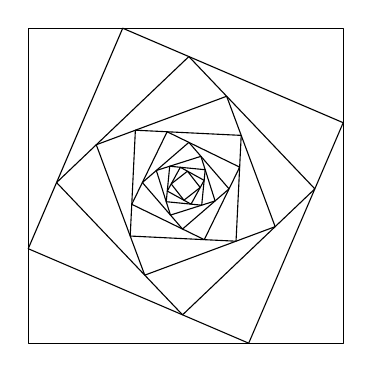
\begin{tikzpicture}[line cap=round,line join=round]
			 \def\a{2}
			\def\t{.7} 
			 \path
				 (-\a,-\a) coordinate (A1)
				(-\a,\a) coordinate  (B1)
				 (\a,\a) coordinate (C1)
				(\a,-\a) coordinate  (D1);
			\draw  (A1)--(B1)--(C1)--(D1)--cycle;
			\foreach  \i[count=\j from 2] in {1,...,10}
			 \draw
				 (barycentric cs:A\i=\t,B\i=1-\t) coordinate (A\j)--
				(barycentric  cs:B\i=\t,C\i=1-\t) coordinate (B\j)--
				(barycentric  cs:C\i=\t,D\i=1-\t) coordinate (C\j)--
				(barycentric cs:D\i=\t,A\i=1-\t)  coordinate (D\j)--cycle;
		\end{tikzpicture}
	 }
	\shortans{42,7} 
	 \loigiai{
		Gọi hình vuông $C_1$ có cạnh $a_1=4$ và có  diện tích là $S_1=a_1^2$.\\
		Cạnh của hình vuông $C_2$ là $a_2=\sqrt{{{\left(  \dfrac{3}{4}{a_1} \right)}^2}+{{\left( \dfrac{1}{4}{a_1} \right)}^2}}=\dfrac{a_1\sqrt{10}}{4}$.\\
		Diện  tích của hình vuông $C_2$ là $S_2=\dfrac{5}{8}{a_1}^2=\dfrac{5}{8}{S_1}$.\\
		Cạnh của hình vuông $C_3$ là $a_3=\sqrt{{{\left( \dfrac{3}{4}{a_2}  \right)}^2}+{{\left( \dfrac{1}{4}{a_2} \right)}^2}}=\dfrac{a_2\sqrt{10}}{4}=a_1.{{\left( \dfrac{\sqrt{10}}{4} \right)}^2}$.\\
		Diện tích của  hình vuông $C_3$ là $S_3={{\left( \dfrac{5}{8} \right)}^2}{a_1}^2={{\left( \dfrac{5}{8} \right)}^2}{S_1}$.\\
		Lý luận tương tự ta có dãy các hình vuông $C_1,\,C_2,\,C_3,\ldots,C_n,\ldots$ có các diện tích lần lượt là $S_1,\,S_2,\,S_3,\ldots,S_n,\ldots$ tạo thành một cấp số nhân lùi vô hạn với số hạng đầu  là: $u_1=S_1=16$ và công bội $q=\dfrac{5}{8}$.\\
		Vậy tổng diện tích của các hình  vuông là\\
	$S=S_1+\,S_2+\,S_3+\ldots+S_n+\ldots=\dfrac{u_1}{1-q}=\dfrac{16}{1-\tfrac{5}{8}}=\dfrac{128}{3}\approx  42{,}7$.}
\end{ex}

% nguồn: Ok_TraLoiNgan_Lop11_Lan1
\begin{ex}%[1D2V3-8]%[ma:42b2701a]
	Một người nhảy bungee (một trò chơi mạo hiểm mà người chơi nhảy từ một nơi có địa thế cao xuống với dây đai an toàn buộc xung quanh người) từ một cây cầu và căng một sợi dây dài $100~ \mathrm{m}$. Sau mỗi lần rơi xuống, nhờ sự đàn hồi của dây, người nhảy được kéo lên một quãng đường có độ  dài bằng $75 \%$ so với lần rơi trước đó và lại bị rơi xuống đúng bằng quãng đường vừa được kéo lên. Tính tổng quãng đường người đó đi được sau $10$ lần kéo lên và lại rơi xuống (đơn vị: mét, làm tròn đến hàng đơn vị).
	 \shortans{377}
	 \loigiai{
		Gọi $u_n$ là độ  dài dây kéo sau $n$ lần rơi xuống $(n \in \mathbb{N})$.\\
		Ta  có $u_0=100~(\mathrm{m})$.\\
		Sau lần rơi đầu tiên độ dài  dây kéo còn lại là $u_1=100\cdot 75 \%~(\mathrm{m})$.\\
		 Sau cú nhảy tiếp theo độ dài dây kéo còn lại là $u_2=100\cdot 75 \% \cdot 75 \%=100 \cdot (75 \%)^2~(\mathrm{m})$.\\
		$\ldots\ldots\ldots\ldots\ldots\ldots\ldots$\\ 
		Dãy số này lập thành một cấp số nhân có  số hạng đầu là $100$ và công bội $q=0{,}75 \%$, có công thức tổng quát $u_n=100 \cdot(0{,}75 \%)^{n-1}~(\mathrm{m})$.\\
		Tổng quãng đường người đó đi được  sau $10$ lần kéo lên và lại rơi xuống là
		 $$
		S_{10}=\dfrac{100\left(1-(75 \%)^{10}\right)}{1-75 \%} \approx 377~(\mathrm{m}). 
	 $$}
\end{ex}

% nguồn: Ok_TraLoiNgan_Lop11_Lan1
\begin{ex}%[1D2V3-8]%[ma:57caad68]
	Vào năm $2023$, dân số của Philippines là $118\,223\,042$ người và tốc độ tăng trưởng dân số là $1{,}5\%$. Nếu tốc độ tăng trưởng dân số này được giữ nguyên hằng năm, hãy ước tính dân số của Philippines vào năm $2030$ là bao  nhiêu triệu người (làm tròn đến hàng đơn vị). (Nguồn: https://danso.org/philippines/).
	 \shortans{131}
	 \loigiai{
		Đây  là bài toán cấp số nhân.\\
		Giả sử dân số của Philippines là N. Vì tốc độ tăng trưởng dân số là $1{,}5\%$ nên sau một năm, số dân  tăng thêm là $1{,}5\% \cdot N$.\\
		Vậy dân số của Philippines vào năm sau là $N + 1{,}5\%  \cdot N = 101{,}5\% \cdot N = 1{,}015N$.\\
		Như vậy, dân số của Philippines sau mỗi năm lập thành một cấp số nhân với  số hạng đầu $u_1 = N$ và công bội $q = 1{,}015$.\\
		Theo bài ra ta  có $u_1 = 118\,223\,042$ ứng với năm $2023$.\\
		 Ta có $2030-2023 = 7$.\\
		Dân số của Philippines vào năm $2030$ chính là dân số của quốc  gia sau $7$ năm kể từ năm $2023$, ứng với $u_8$ và ${{u}_{8}}={{u}_{1}}\cdot{{q}^{8-1}}=118\,223\,042\cdot{{\left( 1{,}015 \right)}^{8-1}}\approx 131\,209\,242$ (người) hay $131$ (triệu người).
	} 
\end{ex}

% nguồn: Ok_TraLoiNgan_Lop11_Lan1
\begin{ex}%[1D2V3-8]%[ma:7bf89550]
	Một công ty xây dựng mua một chiếc máy ủi với giá  $3$ tỉ đồng. Cứ sau mỗi năm sử dụng, giá trị của chiếc máy ủi này lại giảm $20 \%$ so với giá trị của nó trong năm liền trước đó. Giá trị còn lại của chiếc máy ủi đó sau $5$ năm sử dụng là bao nhiêu triệu đồng?
	\shortans{480} 
	\loigiai{ 
		 Gọi $(u_n)$ là dãy số biểu diễn giá trị của chiếc máy ủi theo từng năm. \\
		Dãy số này là một cấp số nhân có  $u_1=3$, $q=0{,}2$.\\
		Số hạng tổng quát của cấp  số nhân này là $u_n=3\cdot 0{,}2^{n-1}$.\\
		Ta có $u_5=3\cdot 0{,}2^4=\dfrac{3}{325}=4{,}8\cdot10^{-3}$.\\ 
		Tương ứng giá trị của chiếc  máy ủi sau $5$ năm là $480$ triệu đồng.
	} 
\end{ex}

% nguồn: Ok_TraLoiNgan_Lop11_Lan1
\begin{ex}%[1D2V3-8]%[ma:f3573510]
	Do ảnh hưởng của dịch Covid $19$ nên doanh  thu $6$ tháng đầu năm của công ty $A$ không đạt kế hoạch. Cụ thể, doanh thu $6$ tháng đầu năm đạt $20$ tỷ đồng, trong đó tháng $6$ đạt $ 6$ tỷ đồng. Để đảm bảo doanh thu cuối năm đạt được kế hoạch năm, công ty đưa ra chỉ tiêu: kể từ tháng $7$ mỗi tháng phải tăng doanh thu so với tháng kề trước $10 \%$. Hỏi theo chỉ tiêu đề ra thì doanh thu cả năm của công ty $A$ đạt được là bao nhiêu tỷ đồng (làm tròn đến một chữ số thập phân)?
	 \shortans{70,9}
	\loigiai{Ta  có\\
		Doanh  thu của công ty trong tháng $7$ là $\mathrm{T}_7=6 \cdot (1+10 \%)$;\\
		Doanh thu của công ty trong tháng  $8$ là $ \mathrm{T}_8=6 \cdot(1+10 \%)^2$;\\
		 $\dots$\\
		Doanh thu của công ty trong tháng $12$ là $ \mathrm{T}_{12}=6 \cdot(1+10 \%)^6$;\\ 
		Do đó, theo chỉ tiêu đề ra  thì doanh thu cả năm của công ty $A$ đạt được là
		$$T=20+6 \cdot(1+10 \%)+6 \cdot(1+10 \%)^2+\ldots +6 \cdot(1+10 \%)^6=20+6 \cdot(1+10  \%) \cdot \dfrac{(1+10 \%)^6-1}{10 \%} \approx 70{,}9.$$
	} 
\end{ex}

% nguồn: Ok_TraLoiNgan_Lop11_Lan1
\begin{ex}%[1D2V3-8]%[ma:0c318a5a]
	Tỉnh Trà Vinh năm $2022$ có dân số là $1\,019\,258$ người  và tốc độ gia tăng dân số trung bình mỗi năm là $0{,}06$ \%. Dự đoán dân số của tỉnh Trà Vinh năm $2030$ là bao nhiêu (Làm tròn kết quả đến hàng phần nghìn)?
	 \shortans{1,02}
	 \loigiai{
		Đây là cấp số nhân  với $u_1 = 1\,019\,258$, công bội $q=1{,}06$. \\
		Năm $2030$ là năm thứ  $9$, tức là dân số tỉnh Trà Vinh năm $2030$ dự đoán là\\ \centerline{$u_9 = u_1\cdot q^{9-1} = 1\,019\,258 \cdot \left(1+\dfrac{0{,}06}{100}\right)^{8} = 1\,024\,160{,}725\approx 1\,024$ nghìn người.}
	 }
\end{ex}

% nguồn: Ok_TraLoiNgan_Lop11_Lan1
\begin{ex}%[1D2V3-8]%[ma:dd82dd9d]
	Một người bắt đầu đi làm được nhận được số tiền lương là $7$ triệu đồng một tháng. Sau $36$ tháng người đó được tăng lương  $7\%$. Hằng tháng người đó tiết kiệm $20 \%$ lương để gửi vào ngân hàng với lãi suất $0,3\%$/tháng theo hình thức lãi kép (nghĩa là lãi của tháng này được nhập vào vốn của tháng kế tiếp). Biết rằng người đó nhận lương vào đầu tháng và số tiền tiết kiệm được chuyển ngay vào ngân hàng.\\
	Hỏi sau $36$ tháng tổng số tiền người đó tiết kiệm được (cả vốn lẫn lãi) là bao nhiêu? (kết quả làm tròn đến hàng phần  chục)
	\shortans{53,3} 
	\loigiai{ 
		Đặt $a=7$ (triệu đồng), $m=20 \%, n=0,3 \%, t=7  \%$. \\
		Hết tháng thứ nhất, người  đó có tổng số tiền tiết kiệm là
		$$T_1=a m(1+n)^1.$$ 
		Hết tháng thứ hai, người đó có  tổng số tiền tiết kiệm là
		 $$T_2=\left(T_1+a m\right)(1+n)=a m(1+n)^2+a m(1+n)^1.$$
		Hết tháng thứ 36, người đó có  tổng số tiền tiết kiệm là
		\begin{align*}
			 T_{36}&=a m(1+n)^{36}+a m(1+n)^{35}+\ldots+a m(1+n) \\
			 & =a m \cdot(1+n) \frac{(1+n)^{36}-1}{n}.
		\end{align*}
		Thay số  ta được $T_{36} \approx 53{,}3$ (triệu đồng).
	} 
\end{ex}

% nguồn: Ok_TraLoiNgan_Lop11_Lan1
\begin{ex}%[1D2V3-8]%[ma:8e55d8bf]
	Anh Bảo làm việc tại công ty S năm đầu tiên với mức lương khởi điểm là $6$ triệu đồng/tháng. Từ năm thứ hai trở đi, mỗi năm lương của anh Bảo tăng thêm $15\%$ so với lương của năm trước  đó. Hỏi tổng số tiền lương anh Bảo nhận được sau $5$ năm làm việc là $a$ triệu đồng. Tìm $a$ (làm tròn kết quả đến hàng đơn vị).
	 \shortans{485}
	\loigiai{ 
		 Tiền lương năm đầu anh Bảo nhận được là $ 6\,000\,000 \cdot 12=72\,000\,000 $ đồng.\\
		Số tiền lương của mỗi năm lập thành cấp số nhân với số hạng đầu $ u_1=72\,000\,000  $, công bội $ q=115\%=1{,}15 $.\\
		Tổng số tiền lương anh Bảo nhận được trong $ 5 $  năm làm việc là \\
		$ S_5=\dfrac{72\,000\,000 \cdot \left(1-1{,}15^5\right)}{1-1{,}15}\approx 485\,000\,000 $  (đồng) $ \approx 485 $ (triệu đồng).
	} 
\end{ex}

% nguồn: Ok_TraLoiNgan_Lop11_Lan1
\begin{ex}%[1D2V3-8]%[ma:941c9d2e]
	Một du khách vào chuồng đua ngựa đặt cược, lần đầu  đặt $50\,000$ đồng, mỗi lần sau đặt gấp đôi lần cọc trước. Người đó thua $10$ lần liên tiếp và thắng ở lần thứ $11$. Hỏi du khách trên thắng hay thua bao nhiêu tiền (đơn vị nghìn đồng)?
	\shortans{50} 
	 \loigiai{
		Số lần  đặt cược tạo thành một cấp số nhân với số hạng đầu $u_1=50\,000$ và công bội $q=2$.\\
		Du khách thua trong $10$  lần liên tiếp nên tổng số tiền thua là
		$${S_{10}}=u_1+u_2+\cdots+{u_{10}}=u_1\cdot\dfrac{1-{q^{10}}}{1-q}=50\,000\cdot\dfrac{1-2^{10}}{1-2}=51\,150\,000.$$ 
		Số tiền  du khách thắng trong lần thứ $11$ là $u_{11}=u_1\cdot q^{10}=50000\cdot2^{10}=51\,200\,000$.\\
		Ta có $u_{11}-S_{10}=51200000-51150000=50\,000$ nên du khách đó thắng  $50\,000$ đồng.
	} 
\end{ex}

% nguồn: Ok_TraLoiNgan_Lop11_Lan1
\begin{ex}%[1D2V3-8]%[ma:1828bf14]
	Một thợ thủ công muốn vẽ trang trí trên một hình vuông kích thước $4$ m $\times$ $4 $  m bằng cách vẽ một hình vuông mới với các đỉnh là trung điểm các cạnh của hình vuông ban đầu, và tô kín màu lên hai tam giác đối diện (tham khảo hình vẽ). Quá trình vẽ và tô theo quy luật đó được lặp lại $5$ lần. Tính số tiền (nghìn đồng) nước sơn để người thợ thủ công đó hoàn thành trang trí hình vuông như trên. Biết tiền nước sơn để sơn $1$ m$^2$ là $50\, 000$ đ.
	\newcommand{\fillhv}[2] 
	{ 
	\draw[fill=maumot,rotate=#2] (-#1,0) coordinate  (A)|-(0,-#1) coordinate (B)--cycle;
	 \draw[fill=mauhai,rotate=#2] (#1,0)coordinate (C)|-(0,#1) coordinate (D)--cycle;
	\draw[rotate=#2] (#1,#1) rectangle  (-#1,-#1);
	} 
	\begin{center}
		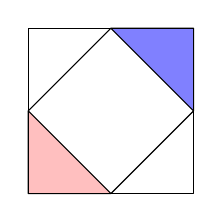
\begin{tikzpicture}[scale=.35,line cap=round,line join=round,rotate=45]
				\def\a{3} 
				\pgfmathsetmacro{\b}{\a/sqrt (2)} 
				\pgfmathsetmacro{\c}{\b/sqrt  (2)}
				\pgfmathsetmacro{\d}{\c/sqrt  (2)}
				\colorlet{maumot}{pink} 
				\colorlet{mauhai}{blue!50} 
				\fillhv{\a}{-45} 
				 \draw (A)--(D)
					 (B)--(C);
			\end{tikzpicture}
		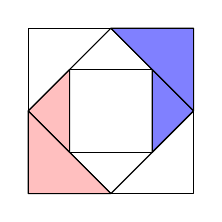
\begin{tikzpicture}[scale=.35,line cap=round,line join=round,rotate=45]
				\def\a{3} 
				 \pgfmathsetmacro{\b}{\a/sqrt (2)}
				\pgfmathsetmacro{\c}{\b/sqrt (2)} 
				\pgfmathsetmacro{\d}{\c/sqrt (2)} 
				 \colorlet{maumot}{pink}
				\colorlet{mauhai}{blue!50} 
				\fillhv{\a}{-45} 
				 \fillhv{\b}{-90}
				\draw (A)--(D) 
					(B)--(C); 
			\end{tikzpicture}
		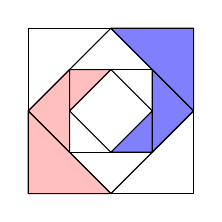
\begin{tikzpicture}[scale=.35,line cap=round,line join=round,rotate=45]
				 \def\a{3}
				\pgfmathsetmacro{\b}{\a/sqrt  (2)}
				\pgfmathsetmacro{\c}{\b/sqrt  (2)}
				\pgfmathsetmacro{\d}{\c/sqrt  (2)}
				 \colorlet{maumot}{pink}
				 \colorlet{mauhai}{blue!50}
				 \fillhv{\a}{-45}
				\fillhv{\b}{-90} 
				\fillhv{\c}{-135} 
				\draw (A)--(D) 
					 (B)--(C);
			\end{tikzpicture}
		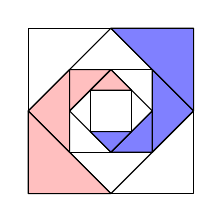
\begin{tikzpicture}[scale=.35,line cap=round,line join=round,rotate=45]
				 \def\a{3}
				 \pgfmathsetmacro{\b}{\a/sqrt (2)}
				\pgfmathsetmacro{\c}{\b/sqrt  (2)}
				\pgfmathsetmacro{\d}{\c/sqrt (2)} 
				 \colorlet{maumot}{pink}
				 \colorlet{mauhai}{blue!50}
				\fillhv{\a}{-45} 
				\fillhv{\b}{-90} 
				\fillhv{\c}{-135} 
				 \fillhv{\d}{-180}
				\draw  (A)--(D)
					 (B)--(C);
			\end{tikzpicture}
	\end{center}
	 \shortans{375}
	\loigiai{ 
		Xét trong $1$ hình vuông  ta thấy diện tích $2$ hình tam giác được tô bằng $\dfrac{1}{4}$ diện tích hình vuông đó, hình vuông được vẽ bằng cách nêu ra trong đề bài có diện tích bằng $\dfrac{1}{2}$ diện tích hình vuông ban đầu. \\
		Đánh số các hình vuông từ ngoài vào trong là $1,2,3,4,5$. Gọi diện tích hình vuông thứ $i$ là $S_i$, diện tích tam giác có cạnh nằm trên cạnh của hình vuông  thứ $i$ là $u_i$, ta có $$u_1 =\dfrac{S_1}{4}, S_2= \dfrac{1}{2}S_1, u_2 =\dfrac{S_2}{4} = \dfrac{S_1}{8},\cdots.$$
		Vậy diện tích  cần sơn là $$ 4 \cdot \dfrac{1- \left( \dfrac{1}{2}\right)^4 }{1-\dfrac{1}{2}}= \dfrac{15}{2} \left( \text{m}^2\right). $$
		Số  tiền nước sơn là $$\dfrac{15}{2} \cdot 50\, 000 = 375\, 000 \text{(đ)}.$$
	} 
\end{ex}

% nguồn: Ok_TraLoiNgan_Lop11_Lan1
\begin{ex}%[1D2V3-8]%[ma:0d34f0f9]
	Một loại thuốc được dùng mỗi ngày một lần. Lúc đầu nồng độ thuốc trong máu của bệnh nhân tăng nhanh, nhưng mỗi liều kế tiếp có tác dụng ít hơn liều trước đó. Lượng thuốc trong máu ở ngày thứ nhất là $50 \mathrm{~mg}$ và mỗi ngày sau đó giảm chỉ còn một nửa so với ngày kề trước đó. Tính tổng lượng thuốc (tính bằng $\mathrm{~mg}$) trong máu của bệnh  nhân sau khi dùng thuốc $10$ ngày liên tiếp (kết quả làm tròn đến hàng phần chục).
	 \shortans{99,9}
	\loigiai{ 
		Lượng thuốc trong máu mỗi ngày của bệnh nhân lập thành cấp số nhân với  số hạng đầu $u_1=50$ và công bội $q=0{,}5$.\\
		Tổng lượng thuốc trong máu $10$ ngày liên tiếp chính là tổng $10$ số hạng đầu của cấp số nhân  này và bằng
		$$ 
		S_{10}=\dfrac{50\left(1-0{,}5^{10}\right)}{1-0{,}5}  \approx 99{,}9\text{~mg}.
		$$ 
	} 
\end{ex}

% nguồn: Ok_TraLoiNgan_Lop11_Lan1
\begin{ex}%[1D2V3-8]%[ma:7b2fc598]
	Theo báo cáo của Chính phủ, dân số của nước ta tính  đến tháng $12$ năm $2018$ là $95{,}93$ triệu người, nếu tỉ lệ tăng trưởng dân số trung bình hằng năm là $1{,}33\%$ thì dân số nước ta vào tháng $12$ năm $2025$ là bao nhiêu? (Tính theo đơn vị triệu người, làm tròn đến hàng đơn vị)
	\shortans{105} 
	\loigiai{ 
		Theo tỉ lệ tăng trưởng $1,33\%$  thì
		\begin{itemize}
			\item Tháng $12$ năm $2019$,  dân số nước ta là:\\
			$u_1=95{,}93+95{,}93\cdot\dfrac{1{,}33}{100}=95{,}93\left(1+\dfrac{1{,}33}{100}\right)$ (triệu  người).
			\item Tháng $12$ năm $2020$, dân số nước  ta là\\
			$\begin{aligned}
			u_2&=95{,}93\left(1+\dfrac{1{,}33}{100}\right)+95{,}93\left(1+\dfrac{1{,}33}{100}\right)\cdot\dfrac{1{,}33}{100}\\&=95{,}93\left(1+\dfrac{1{,}33}{100}\right)\left(1+\dfrac{1{,}33}{100}\right)=95{,}93\left(1+\dfrac{1{,}33}{100}\right)^2 \text{ (triệu  người)}.
		\end{aligned}$
		 \item Theo quy luật đó, ta biết dân số nước ta vào tháng $12$ năm thứ $n$ kể từ năm $2019$ được tính theo công thức $u_n=95{,}93\left(1+\dfrac{1{,}33}{100}\right)^n$ (triệu người).
		\item Vậy vào tháng $12$ năm $2025$  (tức $n=2025-2018=7$), dân số nước ta là\\
		 $$u_7=95{,}93\left(1+\dfrac{1{,}33}{100}\right)^7\approx 105\text{ (triệu người)}.$$
\end{itemize}}
\end{ex}

% nguồn: Ok_TraLoiNgan_Lop11_Lan1
\begin{ex}%[1D2V3-8]%[ma:faf90353]
	Theo báo  cáo của Chính phủ, dân số của nước ta tính đến tháng 12 năm 2018 là $95{,}93$ triệu người, nếu tỉ lệ tăng trưởng dân số trung bình hằng năm là $1{,}33\%$ thì dân số nước ta vào tháng 12 năm 2025 là bao nhiêu? (kết quả làm tròn đến hàng triệu).
	 \shortans{105}
	 \loigiai{
		Theo tỉ lệ tăng trưởng dân số trung bình hằng năm là $1{,}33\%$  thì ta có:\\
		$-$ Tháng 12 năm  2019, dân số nước ta là \\
		 $u_1=95{,}93 + 95{,}93\cdot 1{,}33\%= 95{,}93\left(1 + 0{,}0133\right) =95{,}93\cdot 1{,}0133$.\\
		$-$  Tháng 12 năm 2020, dân số nước ta là \\
		$u_2=(95{,}93\cdot 1{,}0133) + (95{,}93\cdot 1{,}0133)\cdot 0{,}0133  =95{,}93\cdot 1{,}0133\%= 95{,}93\cdot 1{,}0133^2$.\\
		$-$ Tương tự ta có, tháng 12 năm 2021, dân số nước ta là $u_3=95{,}93\cdot  1{,}0133^3$.\\
		$-$ Theo quy luật đó, ta biết dân số nước ta vào tháng 12 năm thứ  $n$ kể từ năm 2019 là $u_n= 95{,}93\cdot 1{,}0133^n$ với $n$ nguyên dương, $n \ge 1$.\\
		$-$ Vậy Tháng 12 năm 2025, dân số nước  ta là $u_7= 95{,}93\cdot 1{,}0133^7 \approx 105$ triệu người.
	} 
\end{ex}

% nguồn: Ok_TraLoiNgan_Lop11_Lan1
\begin{ex}%[1D2V3-8]%[ma:7c7b7d92]
	Một quả bóng được thả thẳng  đứng từ độ cao $10$m rơi xuống đất và nảy lên. Giả sử sau mối một lần rơi xuống, nó nảy lên được một độ cao bằng $75\%$ độ cao vừa rơi xuống. Tính tổng quãng đường quả bóng di chuyển được kể từ lúc thả xuống đến khi quả bóng chạm đất lần thứ $10$ (làm tròn kết quả đến hàng phần mười của mét).
	 \shortans{65,5}
	 \loigiai{
		Gọi $u_n$(m) là độ cao mà quả bóng đạt được sau  khi nảy lên ở lần thứ $n$. \\
		Ta có $u_1=10\cdot 0{,}75=7{,}5$. Ta có, dãy $(u_n)$ lập thành cấp số nhân  có $u_1=7{,}5$ và công bội $q=0{,}75$. Kể từ lúc thả xuống đến khi quả bóng chạm đất lần thứ $10$, quả bóng đã được nảy lên $9$ lần rồi lại rơi xuống.\\
		Do quãng đường quả bóng nảy lên và rơi xuống bằng nhau nên tổng quãng đường quả bóng di chuyển được kể từ lúc thả xuống đến  khi quả bóng chạm đất lần thứ $10$ là
		\[S=10+2\left(u_1+u_2+\cdots+u_9\right)=10+2 \cdot 7{,}5 \cdot \dfrac{1-(0{,}75)^9}{1-0{,}75}  \approx 65{,}5\text{ (m)}.\]
	 }
\end{ex}

% nguồn: Ok_TraLoiNgan_Lop11_Lan1
\begin{ex}%[1D2V3-8]%[ma:7b81b99a]
	Một hãng taxi X áp dụng mức giá đối với khách hàng theo hình thức bậc thang như sau: mỗi bậc áp dụng cho $10$ km. Bậc $1$ (áp dụng cho $10$ km đầu) có giá $10000$ đồng $/1$ km, giá mỗi km ở các bậc tiếp theo giảm $5\%$ so với giá của bậc trước đó. Bạn Toàn thuê hãng taxi X đó để đi hết quãng đường $42$ km. Tính số tiền(ngàn đồng) mà bạn Toàn  phải trả (kết quả làm tròn đến hàng nghìn).
	\shortans{387} 
	\loigiai{ 
		Gọi $T_1$ là giá của mỗi km  ở bậc $1$.\\
		\hspace*{1.5em} $T_2$ là giá của mỗi km  ở bậc $2$.\\
		\hspace*{1.5em} $T_3$ là giá của mỗi km ở bậc  $3$.\\
		\hspace*{1.5em} $T_4$  là giá của mỗi km ở bậc $4$.\\
		\hspace*{1.5em} $T_5$ là giá của mỗi  km ở bậc $5$.\\
		Ta thấy, dãy $T_n (1 \le n \le 5)$ là một cấp số nhân, với  số hạng đầu $T_1=10000$ và công bội $q=\dfrac{95}{100}$.\\
		 Số tiền mà bạn Toàn phải trả trong $40$ km đầu là $$10(T_1+T_2+T_3+T_4)=10\cdot\dfrac{T_1(1-q^4)}{1-q}\approx 371000\ \text{đồng}.$$
		Số tiền mà  bạn Toàn phải trả trong $2$ km cuối là $2\cdot T_5=2\cdot T_1\cdot q^4 \approx 16000$ đồng.\\
		Vậy,  tổng số tiền bạn Toàn phải trả là $371000+16000=387000$ đồng.
	 }
\end{ex}

% nguồn: Ok_TraLoiNgan_Lop11_Lan1
\begin{ex}%[1D2V3-8]%[ma:5a1166a5]
	Một loại thuốc được dùng mỗi ngày một lần. Lúc đầu nồng độ thuốc trong máu của bệnh nhân tăng nhanh, nhưng mỗi liều kế tiếp có tác dụng ít hơn liều trước đó. Lượng thuốc trong máu ở ngày thứ nhất là $50 \,\mathrm{mg}$, và mỗi ngày sau đó giảm chỉ còn một nửa so với ngày kề trước đó. Tính tổng lượng thuốc (tính bằng $\mathrm{mg}$) trong máu của bệnh nhân sau khi dùng thuốc $10$ ngày liên tiếp. 
	 \shortans{99,9}
	\loigiai{ 
		Gọi $(u_n)$ là dãy số biểu diễn giá trị của lượng thuốc trong máu của bệnh nhân theo từng ngày.  \\
		Dãy số này  là một cấp số nhân có $u_1=50$, $q=\dfrac{1}{2}$.\\
		Tổng của $n$ số  hạng đầu tiên của cấp số nhân là $S_n=u_1\dfrac{1-q^n}{1-q}$.\\
		Theo  bài toán, ta có $S_{10}=50 \cdot\dfrac{1-\left(\dfrac{1}{2}\right)^{10}}{1-\dfrac{1}{2}} \approx 99{,}902$.\\
		Vậy tổng lượng thuốc trong máu của bệnh nhân sau khi dùng  thuốc $10$ ngày liên tiếp là $99{,}9$ mg.
	} 
\end{ex}

% nguồn: Ok_TraLoiNgan_Lop11_Lan2
\begin{ex}%[1D2V3-8]%[ma:6214a3d9]
	Để tích lũy tiền cho việc học đại học  của con gái, cô Hoa quyết định hằng tháng bỏ ra $500$ nghìn đồng vào tài khoản tiết kiệm, được trả lãi $0{,}5\%$ cộng dồn hằng tháng. Cô bắt đầu chương trình tích lũy này khi con gái cô tròn $3$ tuổi. Khi cô ấy tích lũy được tiền vào thời điểm gửi khoản tiền thứ $180$ thì lúc này tổng số tiền tiết kiệm được là bao nhiêu triệu đồng? (làm tròn kết quả đến hàng đơn vị)
	 \shortans{145}
	\loigiai{ 
	Gọi $u_n$ là số triệu đồng mà cô Hoa có trong chương trình tích  lũy ở lần gửi thứ n (vào đầu tháng thứ $n$).\\
	Kí hiệu  $a = 0.5$ triệu đồng, $r = 0{,}5\%$.\\
	Số tiền  của cô Hoa trong chương trình ở đầu tháng 1 là $u_1 = a$.\\
	Số tiền của cô Hoa trong chương trình ở đầu tháng 2 là $u_2 =  u_1(1+r)+a$.\\
	Số tiền của cô Hoa trong chương trình ở đầu tháng 3  là $u_3 = u_2(1+r)+a = a(1+r)^2+a(1+r)+a$.\\
	Tương tự cho các tháng tiếp theo, suy ra số tiền của cô Hoa trong chương trình ở đầu tháng n  là:
	$$u_n = a(1+r)^{n-1}+a(1+r)^{n-2}+...+a(1+r)+a = a\dfrac{(1+r)^n-1}{(1+r)-1}=a\dfrac{(1+r)^n-1}{r}.$$ 
	Vào thời điểm gửi khoản tiền thứ 180, cô ấy sẽ tích lũy được $u_{180} = a\dfrac{(1+r)^{180}-1}{r}  \approx 145{,}41$ (triệu đồng).
	} 
\end{ex}

% nguồn: Ok_TraLoiNgan_Lop11_Lan2
\begin{ex}%[1D2V3-8]%[ma:d622719a]
	Từ độ cao $55{,}8$ m của tháp nghiêng Pisa nước Italia, người ta thả một quả bóng cao su chạm xuống đất. Giả sử mỗi lần chạm đất quả bóng lại nảy lên độ cao bằng $\dfrac{1}{10}$ độ cao mà quả bóng đạt  trước đó. Tổng độ dài hành trình của quả bóng được thả từ lúc ban đầu cho đến khi nó nằm yên trên mặt đất bằng bao nhiêu mét?
	 \shortans{68,2}
	\loigiai{ 
	Gọi $h_n$ là độ dài đường đi của quả bóng  ở lần rơi xuống thứ $n$ $(n\in\mathbb{N}^*)$.\\
	Gọi $l_n$ là độ dài đường đi của quả bóng ở lần nảy lên thứ $n$  $(n\in\mathbb{N}^*)$.\\
	 Theo bài ra ta có $h_1=55{,}8$, $l_1=\dfrac{1}{10} \cdot 55{,}8 = 5{,}58$.\\
	Các dãy  số $(h_n)$ và $(l_n)$ là các cấp số nhân lùi vô hạn với công bội $q=\dfrac{1}{10}$.\\
	Từ đó ta suy ra tổng độ dài đường  đi của quả bóng là
	$$S=\dfrac{h_1}{1-\dfrac{1}{10}}+\dfrac{l_1}{1-\dfrac{1}{10}}=\dfrac{10}{9}(h_1+l_1)=68{,}2\;(\text{m}).$$ 
	 }
\end{ex}

% nguồn: Ok_TraLoiNgan_Lop11_Lan2
\begin{ex}%[1D2V3-8]%[ma:21102770]
	Một khay nước có nhiệt độ $20^\circ$C được đặt vào ngăn đá của tủ lạnh. Cho biết sau mỗi giờ,  nhiệt độ của nước đá giảm đi $25$\%. Tính nhiệt độ khay nước đó sau $4$ giờ, làm tròn kết quả đến hàng phần trăm theo đơn vị độ C.
	 \shortans{6,33}
	\loigiai{ 
	Ta có $u_5 = u_1 \cdot q^4 = 20  \cdot 0{,}75^4 \approx 6{,}33^\circ$C.
	 }
\end{ex}

% nguồn: Ok_TraLoiNgan_Lop11_Lan2
\begin{ex}%[1D2V3-8]%[ma:6b99cba9]
	Một loại thuốc được dùng mỗi ngày một lần. Lúc đầu nồng độ thuốc trong máu của bệnh nhân tăng nhanh, nhưng mỗi liều kế tiếp  có tác dụng ít hơn liều trước đó. Lượng thuốc trong máu ở ngày thứ nhất là $50$ mg, và mỗi ngày sau đó giảm chỉ còn một nửa so với ngày kề trước đó. Tính tổng lượng thuốc (tính bằng mg, làm tròn đến hàng đơn vị) trong máu của bệnh nhân sau khi dùng thuốc $10$ ngày liên tiếp.
	 \shortans{100}
	 \loigiai{
	Lượng thuốc trong máu mỗi ngày của bệnh nhân lập thành cấp số nhân với số hạng đầu là 50 và công  bội $q=0{,}5$.\\
	Tổng lượng thuốc trong máu $10$ ngày liên tiếp chính là tổng $10$ số hạng đầu của cấp  số nhân này và bằng $$S_n = \dfrac{50\left[1-(0.5)^{10}\right]}{1-0.5} \approx 99{,}902\;(\text{mg}).$$
	} 
\end{ex}

% nguồn: Ok_TraLoiNgan_Lop11_Lan2
\begin{ex}%[1D2V3-8]%[ma:98560acd]
	Một cây đàn organ có tần số âm thanh các phím liên tiếp tạo thành một cấp số nhân. Cho  biết tần số phím La Trung là $400$ Hz và tần số của phím La Cao cao hơn $12$ phím là $800$ Hz. Tìm công bội của cấp số nhân nói trên (làm tròn kết quả đến hàng phần trăm).
	 \shortans{1,06}
	 \loigiai{
	Ta có $q^{12} = \dfrac{800}{400} = 2$,  suy ra $q \approx 1{,}06$.
	 }
\end{ex}

% nguồn: Ok_TraLoiNgan_Lop11_Lan2
\begin{ex}%[1D2V3-8]%[ma:1652e68a]
	Một công ty xây dựng mua một chiếc  máy ủi với giá $3$ tỉ đồng. Cứ sau mỗi năm sử dụng, giá trị của chiếc máy ủi này lại giảm $20\%$ so với giá trị của nó trong năm liền trước đó. Tìm giá trị còn lại của chiếc máy ủi đó sau $5$ năm sử dụng (kết quả làm tròn đến hàng phần trăm).
	\shortans{1,23} 
	 \loigiai{
		Giá trị của chiếc máy ủi mỗi năm lập thành một cấp số nhân với số hạng đầu bằng $3$  và công bội $q = 1-20\%=0{,}8$.\\
		Giá trị của chiếc máy  ủi sau $5$ năm sử dụng là
		 \[
		u_5  = 3 \times 0{,}8^{5-1} \approx 1{,}23 \text{ (tỉ đồng)}.
		\] 
	 }
\end{ex}

% nguồn: Ok_TraLoiNgan_Lop11_Lan2
\begin{ex}%[1D2V3-8]%[ma:e6f1e726]
	Cho hình vuông $(C_1)$ có cạnh bằng $a$. Người ta chia mỗi cạnh của hình vuông thành bốn phần bằng nhau và nối các điểm chia một cách thích hợp để có hình  vuông $(C_2)$. Từ hình vuông $(C_2)$ lại tiếp tục làm như trên ta nhận được dãy các hình vuông $C_1$, $C_2$, $C_3$, ... ,$C_n$.
	\begin{center}
		\begin{tikzpicture}[scale=1]
				\clip (-0.5,-0.5) rectangle (4,4); 
				\path 
					(0,0) coordinate  (A)
					(4,0) coordinate (B) 
					 ($(A)!1!90:(B)$) coordinate (D)
					($(B)!1!-90:(A)$)  coordinate (C);
				\coordinate (A_1) at  ($(A)!.25!(B)$);
				\coordinate (B_1)  at ($(B)!.25!(C)$);
				\coordinate  (C_1) at ($(C)!.25!(D)$);
				 \coordinate (D_1) at ($(D)!.25!(A)$);
				 \coordinate (A_2) at ($(A_1)!.25!(B_1)$);
				 \coordinate (B_2) at ($(B_1)!.25!(C_1)$);
				\coordinate (C_2) at ($(C_1)!.25!(D_1)$); 
				\coordinate (D_2) at ($(D_1)!.25!(A_1)$); 
				\coordinate (A_3)  at ($(A_2)!.25!(B_2)$);
				\coordinate (B_3)  at ($(B_2)!.25!(C_2)$);
				\coordinate (C_3) at ($(C_2)!.25!(D_2)$); 
				 \coordinate (D_3) at ($(D_2)!.25!(A_2)$);
				\coordinate (A_4)  at ($(A_3)!.25!(B_3)$);
				 \coordinate (B_4) at ($(B_3)!.25!(C_3)$);
				\coordinate (C_4) at ($(C_3)!.25!(D_3)$); 
				\coordinate (D_4)  at ($(D_3)!.25!(A_3)$);
				\coordinate (A_5) at  ($(A_4)!.25!(B_4)$);
				\coordinate (B_5) at  ($(B_4)!.25!(C_4)$);
				\coordinate (C_5) at ($(C_4)!.25!(D_4)$); 
				\coordinate (D_5) at  ($(D_4)!.25!(A_4)$);
				\draw (A)--(B)--(C)--(D)--(A); 
				 \draw (A_1)--(B_1)--(C_1)--(D_1)--(A_1);
				 \draw (A_2)--(B_2)--(C_2)--(D_2)--(A_2);
				\draw  (A_3)--(B_3)--(C_3)--(D_3)--(A_3);
				\draw (A_4)--(B_4)--(C_4)--(D_4)--(A_4); 
				\draw (A_5)--(B_5)--(C_5)--(D_5)--(A_5); 
			\end{tikzpicture}
	\end{center}
	Gọi $S_i$ là diện tích của hình  vuông $C_i$ $(i\in\{1,2,3, \dots\})$. Đặt $T=S_1+S_2+S_3+...+S_n$. Biết $T=\dfrac{32}{3}$. Tính $a$.
	\shortans{2} 
	 \loigiai{
	Cạnh của hình vuông $(C_2)$  là $a_2=\sqrt{\left(\dfrac{3}{4}a\right)^2+\left(\dfrac{1}{4}a\right)^2}=\dfrac{a\sqrt{10}}{4}$. \\
	Do đó diện tích $S_2=\left(\dfrac{a\sqrt{10}}{4}\right)^2 = \dfrac{10a^2}{16} = \dfrac{5}{8}a^2 =  \dfrac{5}{8}S_1$.\\
	Cạnh của hình  vuông $(C_3)$ là $a_3=\sqrt{\left(\dfrac{3}{4}a_2\right)^2+\left(\dfrac{1}{4}a_2\right)^2}=\dfrac{a_2\sqrt{10}}{4}=a\left(\dfrac{\sqrt{10}}{4}\right)^2$. \\
	Do đó diện tích $S_3=\left(a\left(\dfrac{\sqrt{10}}{4}\right)^2\right)^2 = \left(\dfrac{10}{16}\right)^2 a^2 = \dfrac{25}{64}a^2 = \left(\dfrac{5}{8}\right)^2 a^2 =  \dfrac{5}{8}S_2$.\\
	Lý luận tương tự, ta có các $S_1$, $S_2$, $S_3$, ..., $S_n$ tạo thành một dãy cấp số nhân lùi vô hạn có  $u_1=S_1=a^2$ và công bội $q=\dfrac{5}{8}$. \\
	Khi  đó $$T=\dfrac{S_1}{1-q}=\dfrac{a^2}{1-\dfrac{5}{8}}=\dfrac{a^2}{\dfrac{3}{8}}=\dfrac{8a^2}{3}.$$
	Với $T=\dfrac{32}{3}$ ta có $\dfrac{8a^2}{3}=\dfrac{32}{3}\Rightarrow 8a^2=32 \Rightarrow a^2=4\Leftrightarrow a=2$. 
	} 
\end{ex}

% nguồn: Ok_TraLoiNgan_Lop11_Lan2
\begin{ex}%[1D2V3-8]%[ma:5411b5a6]
	Một hình vuông màu vàng có  cạnh 1 đơn vị dài được chia thành chín hình vuông nhỏ hơn và hình vuông ở chính giữa được tô màu xanh. Mỗi hình vuông màu vàng nhỏ hơn lại được chia thành chín hình vuông con, và mỗi hình vuông con ở chính giữa lại được tô màu xanh.
	\begin{center}
		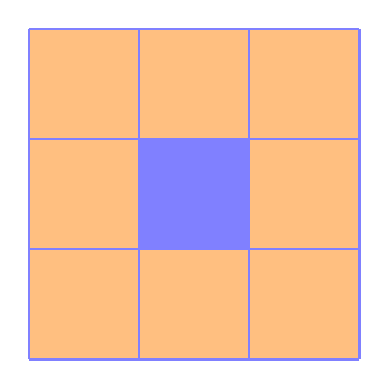
\begin{tikzpicture}[>=stealth,thick,scale=0.7]
				\def\n{1} 
				 \def\a{3}
				\pgfmathsetmacro{\m}{int  (3^(\n))}
				 \def\hv#1{
				 \ifnum#1>0
				\fill[blue!50] (-\a/3,-\a/3) rectangle  (\a/3,\a/3);
				\pgfmathtruncatemacro{\k}{#1-1} 
			\foreach \i in {0,...,3}{\begin{scope}[shift={(90*\i:2)},scale=1/3]\hv{\k}\end{scope}}
			\foreach \i in {0,...,3}{\begin{scope}[shift={(45+90*\i:{4/sqrt (2)})},scale=1/3]\hv{\k}\end{scope}}
				 \fi
				 }
				\fill[orange!50] (-\a,-\a) rectangle (\a,\a); 
				 \hv{\n}
				\foreach \i in  {0,1,...,\m}{
					 \draw[blue!50]
					({-\a+2*\i *\a/\m},\a)--++(270:2*\a) 
					(\a,{-\a+2*\i  *\a/\m})--++(180:2*\a);
				} 
			\end{tikzpicture}
		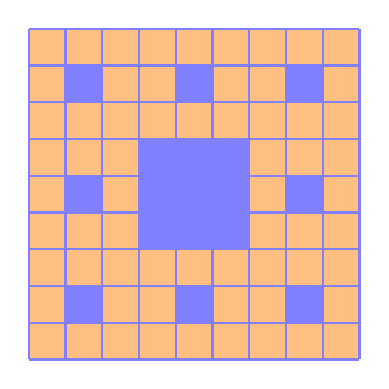
\begin{tikzpicture}[>=stealth,thick,scale=0.7]
				 \def\n{2}
				\def\a{3} 
				\pgfmathsetmacro{\m}{int (3^(\n))} 
				\def\hv#1{ 
				\ifnum#1>0 
				\fill[blue!50] (-\a/3,-\a/3)  rectangle (\a/3,\a/3);
				\pgfmathtruncatemacro{\k}{#1-1} 
			\foreach \i in {0,...,3}{\begin{scope}[shift={(90*\i:2)},scale=1/3]\hv{\k}\end{scope}}
			\foreach \i in {0,...,3}{\begin{scope}[shift={(45+90*\i:{4/sqrt (2)})},scale=1/3]\hv{\k}\end{scope}}
				\fi 
				} 
				\fill[orange!50] (-\a,-\a) rectangle (\a,\a); 
				 \hv{\n}
				\foreach \i in {0,1,...,\m}{ 
					\draw[blue!50] 
					({-\a+2*\i *\a/\m},\a)--++(270:2*\a) 
					(\a,{-\a+2*\i *\a/\m})--++(180:2*\a); 
				 }
			\end{tikzpicture}
		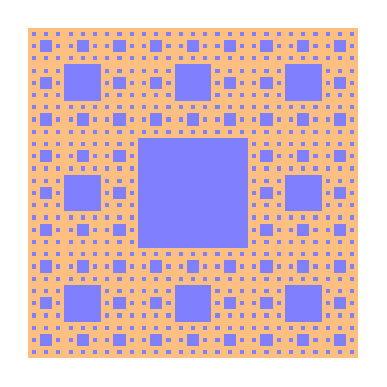
\begin{tikzpicture}[>=stealth,thick,scale=0.7]
				 \def\n{4}
				\def\a{3} 
				\def\hv#1{ 
				\ifnum#1>0 
				\fill[blue!50] (-\a/3,-\a/3) rectangle (\a/3,\a/3); 
				\pgfmathtruncatemacro{\k}{#1-1} 
			\foreach \i in {0,...,3}{\begin{scope}[shift={(90*\i:2)},scale=1/3]\hv{\k}\end{scope}}
			\foreach \i in {0,...,3}{\begin{scope}[shift={(45+90*\i:{4/sqrt (2)})},scale=1/3]\hv{\k}\end{scope}}
				\fi 
				 }
				\fill[orange!50] (-\a,-\a) rectangle (\a,\a); 
				\hv{\n} 
			\end{tikzpicture}
	\end{center}
	Nếu quá trình này được tiếp tục lặp lại năm  lần, thì tổng diện tích các hình vuông được tô màu xanh bao nhiêu? (làm tròn kết quả đến hàng phần trăm)
	 \shortans{0,45}
	 \loigiai{
	Diện tích ô vuông màu xanh sau lần phân chia thứ nhất là: $\dfrac{1}{9}$. Số ô vuông màu xanh  được tạo thêm là $8^0$.\\
	Diện tích ô vuông màu xanh sau lần phân chia thứ hai là: $\dfrac{1}{9^2}$, số ô vuông màu xanh được tạo thêm  là $8^1$.\\
	Diện tích ô vuông màu xanh sau  lần phân chia thứ năm là: $\dfrac{1}{9^5}$, số ô vuông màu xanh được tạo thêm là $8^4$.\\
	Tổng diện tích các ô vuông  màu xanh là: $\dfrac{1}{9}+\dfrac{1}{9^2} \cdot 8^1+...+\dfrac{1}{9^5} \cdot 8^4=0{,}445$.
	} 
\end{ex}

% nguồn: Ok_TraLoiNgan_Lop11_Lan2
\begin{ex}%[1D2V3-8]%[ma:f05aaf4f]
	Với hình vuông $A_1B_1C_1D_1$ như hình vẽ bên,  cách tô màu như phần gạch sọc được gọi là cách tô màu “đẹp”. Một nhà thiết kế tiến hành tô màu cho một hình vuông như hình bên, theo quy trình sau:
	\begin{itemize}
		 \item Bước 1: Tô màu “đẹp” cho hình vuông $A_1B_1C_1D_1$.
		\item Bước 2: Tô màu “đẹp” cho hình vuông $A_2B_2C_2D_2$ là hình vuông ở  chính giữa khi chia hình vuông $A_1B_1C_1D_1$ thành 9 phần bằng nhau như hình vẽ.
		\item Bước 3: Tô màu “đẹp” cho hình vuông $A_3B_3C_3D_3$ là hình vuông ở chính giữa khi chia hình vuông $A_2B_2C_2D_2$ thành 9 phần bằng nhau. 
	\end{itemize}
	\begin{center}
		\begin{tikzpicture}[scale=0.8]
				\coordinate (A1) at (0,9); 
				\coordinate (B1) at  (9,9);
				\coordinate (C1) at (9,0); 
				 \coordinate (D1) at (0,0);
				\coordinate (A2) at  (3,6);
				\coordinate (B2) at (6,6); 
				\coordinate  (C2) at (6,3);
				\coordinate (D2) at  (3,3);
				\begin{scope}
					\clip (A1) --  (D1) -- (C1) -- cycle;
					\fill[pattern=north west lines] (A1)  -- (D1) -- (C1) -- cycle;
				\end{scope}
				\fill[white] (A2) -- (D2)  -- (C2) -- cycle;
				\draw[step=1cm,gray,very  thin] (0,0) grid (9,9);
				\draw[thick] (A1) -- (B1) -- (C1) -- (D1)  -- cycle;
				\draw[thick] (A2) -- (B2) -- (C2) --  (D2) -- cycle;
				 \draw[dashed] (A2) -- (C2);
				\foreach \point/\name/\pos  in {
					 A1/$A_1$/above left,B1/$B_1$/above right,
					C1/$C_1$/below  right,D1/$D_1$/below left,
					A2/$A_2$/left,B2/$B_2$/right, 
					C2/$C_2$/below right,D2/$D_2$/below left} 
					 {
				\fill (\point) circle (1pt) node[\pos=2pt] {\name}; 
				} 
			\end{tikzpicture}
	\end{center}
	 \noindent
	Cứ  tiếp tục như vậy. Hỏi cần ít nhất bao nhiêu bước để tổng diện tích phần được tô màu chiếm $49{,}99\%$?
	\shortans{4} 
	 \loigiai{
	Gọi diện tích được tô  màu ở mỗi bước là $u_n$, $n\in\mathbb{N}^*$.\\
	Dễ thấy  dãy các giá trị $u_n$ là một cấp số nhân với số hạng đầu $u_1=\dfrac{4}{9}$ và công bội $q=\dfrac{1}{9}$.\\
	Gọi $S_k$  là tổng của k số hạng đầu trong cấp số nhân đang xét thì $S_k=\dfrac{u_1(q^k-1)}{q-1}$.\\
	Để tổng diện tích phần được tô màu chiếm 49.99\% thì $\dfrac{u_1(q^k-1)}{q-1}\ge0{,}4999\Leftrightarrow k\ge3{,}8$.\\ 
	Vậy cần ít nhất $4$ bước. 
	} 
\end{ex}

% nguồn: Ok_TraLoiNgan_Lop11_Lan2
\begin{ex}%[1D2V3-8]%[ma:bd9bd056]
	Mặt sàn tầng một (tầng trệt) của một ngôi nhà cao hơn mặt sân $0{,}5$ m. Cầu thang đi từ tầng một lên  tầng hai gồm $25$ bậc, mỗi bậc cao $16$ cm. Viết công thức để tìm độ cao của bậc cầu thang thứ $n$ so với mặt sân và tính độ cao của sàn tầng hai so với mặt sân.
	\shortans{4,5} 
	 \loigiai{
	Mỗi bậc thang cao $16~\text{cm} = 0{,}16~\text{m} \Rightarrow n$ bậc  thang cao $0{,}16n$ (m).\\
	Vì mặt bằng sàn cao hơn  mặt sân $0{,}5$ m nên công thức tính độ cao của bậc $n$ so với mặt sân sẽ là $$h_n = (0{,}5+0{,}16n)\;\text{m}.$$
	Khi đó độ cao của sàn tầng hai so với mặt sân ứng với  $n=25$ là $h_{25} = 0{,}5+0{,}16 \cdot 25 = 4{,}5$ m.
	 }
\end{ex}

% nguồn: Ok_TraLoiNgan_Lop11_Lan2
\begin{ex}%[1D2V3-8]%[ma:0d667538]
	Một loại vi khuẩn được nuôi cấy trong ống nghiệm, cứ $20$ phút lại phân đôi một  lần. Nếu ban đầu có $200$ vi khuẩn, tính số lượng vi khuẩn có trong ống nghiệm sau $2$ giờ.
	\shortans{1280} 
	\loigiai{Ta có $2$ giờ $= 120$ phút $= 6\cdot 20$ phút. Do đó  sau $2$ giờ vi khuẩn phân đôi $6$ lần.\\
		Gọi $u_n$ là số lượng vi khuẩn có trong ống nghiệm sau lần phân đôi  thứ $n-1$.\\
		Khi đó, dãy số $\left(u_n  \right)$ là một cấp số nhân với $u_1 = 200$ và $q = 2$.\\
		Ta  có $u_7 = u_1\cdot q^6 = 200\cdot 2^6 = 12\,800$. \\
	Vậy sau $2$ giờ, trong ống nghiệm có  $12\,800$ vi khuẩn.}
\end{ex}

% nguồn: Ok_TraLoiNgan_Lop11_Lan2
\begin{ex}%[1D2V3-8]%[ma:a27b280c]
	Dân số Việt Nam năm $2020$ là khoảng $97{,}6$ triệu người. Nếu trung bình mỗi năm tăng $1{,}14\%$ thì ước tính dân số Việt Nam năm $2040$  là khoảng bao nhiêu triệu người (làm tròn kết quả đến hàng đơn vị)?
	\shortans{122} 
	\loigiai{ 
	Ước tính dân số Việt Nam năm 2040 là $97{,}6 \cdot (1+0{,}0114)^{20} \approx 122{,}4$  (triệu người).
	} 
\end{ex}

% nguồn: Ok_TraLoiNgan_Lop11_Lan2
\begin{ex}%[1D2V3-8]%[ma:468a5c57]
	Để trang trí cho  quán trà sữa sắp mở cửa của mình, bạn Việt quyết định tô màu một mảng tường hình vuông cạnh bằng 1m. Phần tô màu dự kiến là các hình vuông nhỏ được đánh số lần lượt là $1$, $2$, $3$, ... , $n$, trong đó cạnh của hình vuông kế tiếp bằng một nửa cạnh hình vuông trước đó.
	\begin{center}
		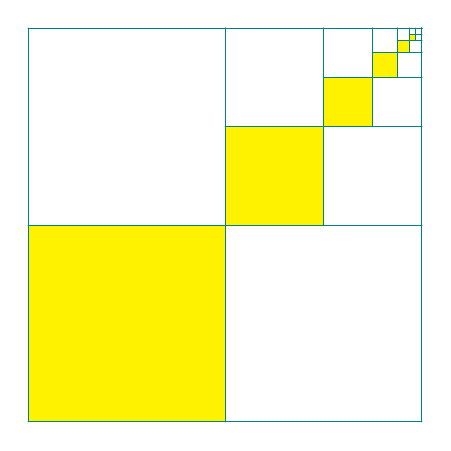
\begin{tikzpicture}[line join=round,line cap=round,teal]
				 \def\m{9}
				\def\a{5} 
				\tikzset{hv/.pic={ 
				 \path[fill=yellow] (0,0) rectangle (0.5*\a,0.5*\a);
				 \draw[step=0.5*\a] (0,0) grid (\a,\a);
					}} 
				 \def\l{0}
				\foreach  \i in {0,...,5}{
					 \pgfmathsetmacro{\n}{\l-(0.5)^\i*sqrt (2)*\a}
					 \path (45:\n) pic[scale={(0.5)^\i}]{hv};
					\global \let \n =  \l;
				} 
			\end{tikzpicture}
	\end{center}
	Giả sử quá trình tô màu của Việt có thể diễn ra nhiều giờ. Hỏi bạn Việt tô màu đến hình vuông thứ mấy thì  diện tích của hình vuông được tô bắt đầu nhỏ hơn $\dfrac{1}{1000}$ m$^2$?
	 \shortans{5}
	 \loigiai{
	Diện tích của hình vuông lập thành cấp  số nhân với số hạng đầu tiên là $u_1=\dfrac{1}{4}$.\\
	Do đó số hạng tổng  quát là $u_n=\dfrac{1}{4}\cdot\left(\dfrac{1}{4}\right)^{n-1}=\dfrac{1}{4^n}\qquad(n\ge1)$.\\
	Để diện tích của hình vuông tô màu nhỏ hơn $\dfrac{1}{1000}\Leftrightarrow\dfrac{1}{4^n}<\dfrac{1}{1000}\Leftrightarrow4^n>1000\Rightarrow n\ge5$.\\ 
	Vậy tô màu từ hình vuông thứ $5$ thỏa mãn  yêu cầu bài toán.
	} 
\end{ex}

% nguồn: Ok_TraLoiNgan_Lop11_Lan2
\begin{ex}%[1D2V3-8]%[ma:ded3f6e3]
	Các cạnh của hình vuông ban đầu có chiều dài $16$ cm. Một hình vuông mới được hình thành bằng cách nối các điểm giữa của các cạnh của hình  vuông ban đầu và hai trong số các hình tam giác kết quả được tô màu (tham khảo hình vẽ dưới).
	\begin{center}
		\begin{tikzpicture}[scale=0.8]
				\foreach \n  [count=\i from 0] in {1,2,3,4}{
					\begin{scope}[xshift=5*\i cm]
					\draw (0,0) rectangle  (4,4);
					\coordinate (A) at  (0,0);
					\coordinate  (B) at (4,0);
					\coordinate  (C) at (4,4);
					\coordinate  (D) at (0,4);
					\coordinate (P0) at  (A);
					 \coordinate (P1) at (B);
					 \coordinate (P2) at (C);
					 \coordinate (P3) at (D);
					 \foreach \k in {1,...,\n}{
					\coordinate (Q0) at  ($(P0)!.5!(P1)$);
					\coordinate  (Q1) at ($(P1)!.5!(P2)$);
					\coordinate (Q2)  at ($(P2)!.5!(P3)$);
					\coordinate  (Q3) at ($(P3)!.5!(P0)$);
					\draw (Q0) -- (Q1) -- (Q2)  -- (Q3) -- cycle;
					\fill[red!60]  (Q0) -- (Q3) -- (P0) -- cycle;
					\fill[blue!60] (Q1) -- (Q2) -- (P2) --  cycle;
					\coordinate  (P0) at (Q0);
					\coordinate (P1) at (Q1); 
					\coordinate (P2) at  (Q2);
					\coordinate (P3) at  (Q3);
				 }
					\end{scope}
				} 
			\end{tikzpicture}
	\end{center}
	Nếu  quá trình này được lặp lại năm lần nữa, hãy xác định tổng diện tích của vùng được tô màu.
	 \shortans{124}
	 \loigiai{
	Gọi $u_n$ là diện tích hai tam  giác được tô màu ở lần thực hiện thứ $n$. \\
	Gọi $a$ là độ  dài cạnh của hình vuông ban đầu.\\
	Ở lần 1 thì độ dài cạnh tam giác  vuông cân là $\dfrac{a}{2}$ nên $u_1 = 2 \cdot \dfrac{1}{2}\cdot \dfrac{a}{2} \cdot\dfrac{a}{2} = \dfrac{a^2}{2^2}$ và độ dài cạnh hình vuông sau đó là $\dfrac{a\sqrt{2}}{2}$.\\
	Ở lần 2  thì độ dài cạnh tam giác vuông cân là $\dfrac{a}{2} \cdot \dfrac{\sqrt{2}}{2}$ nên $u_2 = \dfrac{a^2}{2^3}$.\\
	Ở  lần 3 thì độ dài cạnh tam giác vuông cân là $\dfrac{a}{2} \cdot \dfrac{\sqrt{2}}{2} \cdot \dfrac{\sqrt{2}}{2}$ nên $u_3 = \dfrac{a^2}{2^4}$.\\
	Như vậy, dãy số $(u_n)$ là cấp số nhân với $u_1 = \dfrac{a^2}{4}$ và  công bội $q = \dfrac{1}{2}$.\\
	Tổng diện tích sau năm lần thực hiện là $S_5 =  u_1 \dfrac{1-q^5}{1-q} = 124$ cm$^2$.
	} 
\end{ex}

% nguồn: Ok_TraLoiNgan_Lop11_Lan2
\begin{ex}%[1D2V3-8]%[ma:c0ccc6c6]
	Ban đầu, một quả lắc đồng hồ dao động theo một cung tròn dài $46$ cm. Sau mỗi lần đu liên tiếp, độ dài của cung tròn bằng  $0{,}98$ độ dài cung tròn ở ngay lần trước đó. Sau $15$ lần dao động, quả lắc sẽ đi được quãng đường tổng cộng là bao nhiêu? (Kết quả tính theo centimét và làm tròn đến hàng đơn vị)
	\shortans{601} 
	\loigiai{ 
	Gọi $u_n$ là độ dài cung tròn ở lần thứ $n$  khi con lắc dao động.\\
	Do lần một, quả lắc  đồng hồ dao động theo một cung tròn dài $46$ cm, sau mỗi lần dao động liên tiếp, độ dài của cung tròn bằng $0{,}98$ độ dài cung tròn ở ngay lần trước đó nên dãy số $(u_n)$ lập thành cấp số nhân có $u_1=46$ và công bội $q=0{,}98$.\\
	Sau  $15$ lần dao động, quả lắc sẽ đi được quãng đường tổng cộng là
	$$S_{15} = u_1\dfrac{1-q^{15}}{1-q} = 46\cdot\dfrac{1-0.98^{15}}{1-0.98} \approx  601 \ \text{(cm)}.$$
	 }
\end{ex}

% nguồn: Ok_TraLoiNgan_Lop11_Lan2
\begin{ex}%[1D2V3-8]%[ma:45992d61]
	Tỷ lệ tăng dân số của tỉnh $X$ là $1{,}4\%$. Biết rằng dân số tỉnh $X$ hiện nay là $1{,}8$ triệu người. Hỏi với mức tăng như vậy thì  sau $10$ năm nữa dân số tỉnh $X$ là bao nhiêu? (đơn vị: triệu người và kết quả làm tròn đến hàng phần trăm)
	\shortans{2,07} 
	\loigiai{ 
		Theo giả thiết,  ta thấy tỷ lệ tăng dân số hằng năm của tỉnh $X$ là một cấp số nhân $(u_n)$ với số hạng đầu $u_1 = 1{,}8 \times 10^6$ và công bội
		\[q = 1 + \dfrac{1{,}4}{100} =  1{,}014.\]
		Do đó,  dân số của tỉnh $X$ sau $10$ năm là
		 \[
		u_{11} = u_1 \cdot q^{10} = 1{,}8 \cdot 10^6 \cdot  (1{,}014)^{10} \approx 2{,}07 \text{ triệu người}.
		 \]
	 }
\end{ex}

% nguồn: Ok_TraLoiNgan_Lop11_Lan2
\begin{ex}%[1D2V3-8]%[ma:93b39479]
	Một tháp $10$ tầng có diện tích sàn của tầng dưới cùng là $6\,144$ m$^2$. Tính diện tích mặt sàn tầng trên cùng, biết rằng diện tích mặt sàn mỗi tầng bằng nửa diện tích  mặt sàn tầng ngay bên dưới.
	\shortans{12} 
	\loigiai{ 
	Ta có $u_{10} = u_1 \cdot q^9 = 6\,144 \cdot \left(\dfrac{1}{2}\right)^9 = 12$  m$^2$.
	 }
\end{ex}


%%%%%%%%%%%%%%%% TỰ LUẬN %%%%%%%%%%%%%%%%

% nguồn: Ok_TuanLuan_Toan11_Lan2
\begin{ex}%[1D2H3-8]%[ma:01700bed]
	Người ta thiết kế một cái tháp gồm $11$ tầng. Diện tích bề mặt trên của mỗi tầng bằng nữa  diện tích của mặt trên của tầng ngay bên dưới và diện tích mặt trên của tầng $1$ bằng nửa diện tích của đế tháp. Tính diện tích mặt trên cùng.
	\loigiai{ 
		Diện  tích bề mặt của mỗi tầng lập thành một cấp số nhân có công bội $q=\dfrac{1}{2}$ và $u_1=\dfrac{12288}{2}=6144$.\\ Khi đó diện tích mặt trên cùng là
		\[ 
		u_{11}=u_1  q^{10}=\dfrac{6144}{2^{10}}=6.
		\] 
	} 
\end{ex}

% nguồn: Ok_TuanLuan_Toan11_Lan2
\begin{ex}%[1D2H3-8]%[ma:a7b71ffe]
	Một du khách vào trường đua ngựa đặt cược, lần đầu đặt $20\,000$ đồng, mỗi lần sau tiền đặt gấp đôi lần tiền đặt cọc  trước. Người đó thua $9$ lần liên tiếp và thắng ở lần thứ $10$. Hỏi du khách trên thắng hay thua bao nhiêu?
	\loigiai{ 
		 Số tiền du khách đặt trong mỗi lần là một cấp số nhân có $u_1 = 20\,000$ và công bội $q = 2$.\\
		Du khách thua  trong $9$ lần đầu tiên nên tổng số tiền thua là:
		\[ 
		S_9 = u_1 + u_2 + \ldots + u_9 = \dfrac{u_1 \left(1 - q^9\right)}{1  - q} = \dfrac{20\,000 (1 - 2^9)}{1 - 2} = 1\,022\,0000.
		\] 
		Số tiền mà du khách thắng trong  lần thứ $10$ là
		\[ 
		u_{10} = u_1 \cdot q^9 = 20\,000 \cdot 2^9 =  1\,024\,0000.
		\] 
		Ta có $u_{10} - S_9 = 20\,000  > 0$ nên du khách thắng $20\,000$ đồng.
	 }
\end{ex}

% nguồn: Ok_TuanLuan_Toan11_Lan1
\begin{bt}%[1D2V3-8]%[ma:a9efbd3a]
	\textbf{(0.5  điểm)}Cho hình vuông ${{A}_{1}}{{B}_{1}}{{C}_{1}}{{D}_{1}}$ có độ dài đường chéo bằng $2\sqrt{6}$ (đơn vị độ dài). Chia hình vuông ${{A}_{1}}{{B}_{1}}{{C}_{1}}{{D}_{1}}$ thành $9$ hình vuông nhỏ bằng nhau và tô màu như hình vẽ bên dưới. Với ${{A}_{2}}{{B}_{2}}{{C}_{2}}{{D}_{2}}$ là hình vuông nhỏ chính giữa, lại chia thành $9$ hình vuông nhỏ bằng nhau và tô màu như quy luật trên. Cứ tiếp tục như vậy.
	\begin{center}
		{\begin{tikzpicture}[>=stealth,line join=round,line cap=round,font=\footnotesize,scale=1.3]
		 \draw (0,0)--(0,3)-- (3,3)--(3,0)--(0,0);
		\fill (0,0) circle (1.2pt)  node[below left]{$B_1$};
		\fill (0,3)  circle (1.2pt) node[above left]{$A_1$};
		\fill (3,3) circle  (1.2pt) node[above right]{$D_1$};
		\fill (3,0) circle (1.2pt) node[below right]{$C_1$}; 
		\draw (1.5,-.6) node{\textbf{}}; 
	\end{tikzpicture}
		} 
		{\begin{tikzpicture}[>=stealth,line join=round,line cap=round,font=\footnotesize,scale=1.3]
		\draw (0,3)--(1,2) 
			(3,0)--(2,1); 
		\draw[dashed]  (1,2)--(2,1);
		\fill[pattern=crosshatch dots  light steel blue,smooth] (0,3)--(0,0)--(3,0)--(2,1)--(1,1)--(1,2)--(0,3);
		\draw [step=1,very  thin] (0,0) grid (3,3);
		\fill (0,0) circle (1.2pt)  node[below left]{$B_1$};
		\fill  (0,3) circle (1.2pt) node[above left]{$A_1$};
		\fill (3,3) circle (1.2pt) node[above right]{$D_1$}; 
		\fill (3,0)  circle (1.2pt) node[below right]{$C_1$};
		\fill (1,1)  circle (1.2pt) node[above left]{$B_2$};
		 \fill (1,2) circle (1.2pt) node[above right]{$A_2$};
		\fill (2,2) circle (1.2pt)  node[above right]{$D_2$};
		\fill (2,1)  circle (1.2pt) node[above right]{$C_2$};
		\draw  (1.5,-.5) node{\textbf{Hình 1}};
	\end{tikzpicture}
		} 
		{\begin{tikzpicture}[>=stealth,line join=round,line cap=round,font=\footnotesize,scale=1.3]
		\draw (0,3)--(1.3333333,1.6666667) 
			 (3,0)--(1.6666667,1.3333333);
		\draw[dashed]  (1,2)--(2,1);
		\fill[pattern=crosshatch dots light steel blue,smooth] (0,3)--(0,0)--(3,0)--(2,1)--(1,1)--(1,2)--(0,3); 
		 \fill[pattern=crosshatch dots light steel blue,smooth] (1,2)--(1,1)--(2,1)--(1.6666667,1.3333333)--(1.3333333,1.3333333)--(1.3333333,1.6666667)--(1,2);
		\draw [step=1,very thin] (0,0) grid  (3,3);
		 \draw [step=1/3,very thin] (1,1) grid (2,2);
		\fill (0,0)  circle (1.2pt) node[below left]{$B_1$};
		\fill (0,3) circle (1.2pt)  node[above left]{$A_1$};
		\fill (3,3)  circle (1.2pt) node[above right]{$D_1$};
		 \fill (3,0) circle (1.2pt) node[below right]{$C_1$};
		\fill  (1,1) circle (1.2pt) node[above left]{$B_2$};
		\fill (1,2)  circle (1.2pt) node[above right]{$A_2$};
		\fill (2,2)  circle (1.2pt) node[above right]{$D_2$};
		\fill (2,1) circle (1.2pt) node[above  right]{$C_2$};
		\draw (1.5,-.5)  node{\textbf{Hình 2}};
	\end{tikzpicture}
		 }
	\end{center}
	\begin{enumerate}
		\item Tính diện tích phần đã  tô màu ở \textbf{Hình 1}.
		\item Gọi ${{u}_{1}},{{u}_{2}},\ldots $ lần lượt là diện tích phần tô màu ở hình vuông ${{A}_{1}}{{B}_{1}}{{C}_{1}}{{D}_{1}}$, ${{A}_{2}}{{B}_{2}}{{C}_{2}}{{D}_{2}},\ldots $ Đặt  ${{S}_{n}}={{u}_{1}}+{{u}_{2}}+\cdots +{{u}_{n}}$, tính $\lim {{S}_{n}}$.
	\end{enumerate}
	\loigiai{ 
		\begin{enumerate}
			\item Độ dài  cạnh hình vuông ban đầu đã cho: $2\sqrt{3}$ (đơn vị độ dài)\\
			Diện tích phần đã tô màu lần chia hình đầu tiên:  $4.{{\left( \dfrac{2\sqrt{3}}{3} \right)}^{2}}=\dfrac{16}{3}$.
			\item Theo đề bài, ${{S}_{n}}$ là tổng cấp số nhân với  ${{u}_{1}}=\dfrac{16}{3}$ và công bội $q=\dfrac{1}{9}$, do đó
			$${{S}_{n}}=\dfrac{16}{3}\cdot \dfrac{1-{{\left( \dfrac{1}{9} \right)}^{n}}}{1-\dfrac{1}{9}}=6\cdot \left[1-{{\left( \dfrac{1}{9} \right)}^{n}} \right].$$  Vậy $\lim {{S}_{n}}=6$.
		\end{enumerate}
	} 
\end{bt}

% nguồn: Ok_TuanLuan_Toan11_Lan1
\begin{bt}%[1D2V3-8]%[ma:776c0489]
	Số lượng của loại vi khuẩn A trong một phòng thí nghiệm được tính theo công thức $s(t)=s(0)\cdot 2^t$, trong đó $s(0)$ là số lượng vi khuẩn A lúc ban đầu, $s(t)$ là  số lượng vi khuẩn A có sau $t$ phút. Biết sau $3$ phút thì số lượng vi khuẩn A là $624$ con. Hỏi sau bao lâu, kể từ lúc ban đầu, số lượng vi khuẩn A là $10$ triệu con?
	\loigiai{ 
		Theo giả thiết thì 
		 \[s(3)=624\Leftrightarrow s(0)\cdot 2^3=624\Leftrightarrow s(0)=78{,}125 \,(\text{nghìn con}).\]
		Khi số lượng vi khuẩn là $10$ triệu con  bằng $10000$ nghìn con khi thì
		\[s(0)\cdot 2^t=10000\Leftrightarrow  2^t=\dfrac{10000}{78{,}125}=128=2^7\Rightarrow t=7 \,(\text{phút}).\]
	} 
\end{bt}

% nguồn: Ok_TuanLuan_Toan11_Lan2
\begin{ex}%[1D2V3-8]%[ma:026aae59]
	\textbf{(0.5 điểm)}Cho hình vuông ${{A}_{1}}{{B}_{1}}{{C}_{1}}{{D}_{1}}$ có độ dài  đường chéo bằng $2\sqrt{6}$ (đơn vị độ dài). Chia hình vuông ${{A}_{1}}{{B}_{1}}{{C}_{1}}{{D}_{1}}$ thành $9$ hình vuông nhỏ bằng nhau và tô màu như hình vẽ bên dưới. Với ${{A}_{2}}{{B}_{2}}{{C}_{2}}{{D}_{2}}$ là hình vuông nhỏ chính giữa, lại chia thành $9$ hình vuông nhỏ bằng nhau và tô màu như quy luật trên. Cứ tiếp tục như vậy.
	\begin{center}
		{\begin{tikzpicture}[>=stealth,line join=round,line cap=round,font=\footnotesize,scale=1.3]
		\draw (0,0)--(0,3)--  (3,3)--(3,0)--(0,0);
		\fill (0,0) circle (1.2pt)  node[below left]{$B_1$};
		 \fill (0,3) circle (1.2pt) node[above left]{$A_1$};
		\fill (3,3)  circle (1.2pt) node[above right]{$D_1$};
		\fill (3,0) circle (1.2pt) node[below right]{$C_1$}; 
		 \draw (1.5,-.6) node{\textbf{}};
	\end{tikzpicture}
		} 
		{\begin{tikzpicture}[>=stealth,line join=round,line cap=round,font=\footnotesize,scale=1.3]
		 \draw (0,3)--(1,2)
			(3,0)--(2,1); 
		\draw[dashed] (1,2)--(2,1); 
		\fill[pattern=crosshatch dots  light steel blue,smooth] (0,3)--(0,0)--(3,0)--(2,1)--(1,1)--(1,2)--(0,3);
		\draw [step=1,very thin]  (0,0) grid (3,3);
		\fill (0,0) circle (1.2pt) node[below left]{$B_1$}; 
		\fill (0,3) circle (1.2pt) node[above left]{$A_1$}; 
		\fill (3,3) circle (1.2pt)  node[above right]{$D_1$};
		\fill (3,0) circle  (1.2pt) node[below right]{$C_1$};
		 \fill (1,1) circle (1.2pt) node[above left]{$B_2$};
		\fill (1,2)  circle (1.2pt) node[above right]{$A_2$};
		\fill (2,2) circle  (1.2pt) node[above right]{$D_2$};
		\fill (2,1)  circle (1.2pt) node[above right]{$C_2$};
		 \draw (1.5,-.5) node{\textbf{Hình 1}};
	\end{tikzpicture}
		 }
		{\begin{tikzpicture}[>=stealth,line join=round,line cap=round,font=\footnotesize,scale=1.3]
		\draw  (0,3)--(1.3333333,1.6666667)
			(3,0)--(1.6666667,1.3333333); 
		 \draw[dashed] (1,2)--(2,1);
		\fill[pattern=crosshatch dots  light steel blue,smooth] (0,3)--(0,0)--(3,0)--(2,1)--(1,1)--(1,2)--(0,3);
		\fill[pattern=crosshatch dots light steel blue,smooth] (1,2)--(1,1)--(2,1)--(1.6666667,1.3333333)--(1.3333333,1.3333333)--(1.3333333,1.6666667)--(1,2); 
		\draw [step=1,very thin] (0,0) grid  (3,3);
		\draw [step=1/3,very thin] (1,1) grid  (2,2);
		\fill (0,0) circle  (1.2pt) node[below left]{$B_1$};
		\fill (0,3) circle (1.2pt)  node[above left]{$A_1$};
		\fill (3,3)  circle (1.2pt) node[above right]{$D_1$};
		\fill (3,0) circle (1.2pt) node[below  right]{$C_1$};
		\fill (1,1) circle (1.2pt)  node[above left]{$B_2$};
		\fill (1,2) circle (1.2pt) node[above right]{$A_2$}; 
		\fill (2,2)  circle (1.2pt) node[above right]{$D_2$};
		\fill (2,1) circle (1.2pt)  node[above right]{$C_2$};
		\draw (1.5,-.5) node{\textbf{Hình  2}};
	\end{tikzpicture}
		 }
	\end{center}
	\begin{enumerate}
		\item Tính diện tích phần đã tô màu ở  \textbf{Hình 1}.
		\item Gọi ${{u}_{1}},{{u}_{2}},\ldots $  lần lượt là diện tích phần tô màu ở hình vuông ${{A}_{1}}{{B}_{1}}{{C}_{1}}{{D}_{1}}$, ${{A}_{2}}{{B}_{2}}{{C}_{2}}{{D}_{2}},\ldots $ Đặt ${{S}_{n}}={{u}_{1}}+{{u}_{2}}+\cdots +{{u}_{n}}$, tính $\lim {{S}_{n}}$.
	\end{enumerate}
	 \loigiai{
		\begin{enumerate}
			\item Độ dài cạnh hình vuông ban đầu đã cho: $2\sqrt{3}$ (đơn vị độ  dài)\\
			Diện tích phần đã tô màu lần chia hình  đầu tiên: $4.{{\left( \dfrac{2\sqrt{3}}{3} \right)}^{2}}=\dfrac{16}{3}$.
			\item Theo đề bài, ${{S}_{n}}$ là tổng cấp số nhân với ${{u}_{1}}=\dfrac{16}{3}$ và công bội $q=\dfrac{1}{9}$,  do đó
			$${{S}_{n}}=\dfrac{16}{3}\cdot \dfrac{1-{{\left( \dfrac{1}{9} \right)}^{n}}}{1-\dfrac{1}{9}}=6\cdot \left[1-{{\left(  \dfrac{1}{9} \right)}^{n}} \right].$$ Vậy $\lim {{S}_{n}}=6$.
		\end{enumerate}
	} 
\end{ex}

% nguồn: Ok_TuanLuan_Toan11_Lan2
\begin{ex}%[1D2V3-8]%[ma:de51c7d3]
	Số lượng của loại vi khuẩn A trong một phòng thí nghiệm được tính theo công  thức $s(t)=s(0)\cdot 2^t$, trong đó $s(0)$ là số lượng vi khuẩn A lúc ban đầu, $s(t)$ là số lượng vi khuẩn A có sau $t$ phút. Biết sau $3$ phút thì số lượng vi khuẩn A là $624$ con. Hỏi sau bao lâu, kể từ lúc ban đầu, số lượng vi khuẩn A là $10$ triệu con?
	 \loigiai{
		Theo giả  thiết thì
		\[s(3)=624\Leftrightarrow s(0)\cdot 2^3=624\Leftrightarrow s(0)=78{,}125 \,(\text{nghìn con}).\] 
		Khi số lượng vi khuẩn là $10$ triệu con bằng  $10000$ nghìn con khi thì
		\[s(0)\cdot 2^t=10000\Leftrightarrow 2^t=\dfrac{10000}{78{,}125}=128=2^7\Rightarrow t=7  \,(\text{phút}).\]
	} 
\end{ex}

% nguồn: Ok_TuanLuan_Toan11_Lan2
\begin{ex}%[1D2V3-8]%[ma:8319ddea]
	Chu kì bán rã của nguyên tố phóng xạ poloni $210$ là $138$ ngày. Tính khối lượng còn lại của $20$ gam  poloni $210$ sau $7314$ ngày.
	 \loigiai{
		Kí hiệu $u_n$ là khối lượng còn lại của $20$  gam poloni $210$ sau $n$ chu kì bán rã.\\
		Ta có $7314$ ngày gồm  $53$ chu kì bán rã. Theo đề bài ra, ta cần tính $u_{53}$.\\
		Từ giả thiết suy ra dãy  $\left(u_n\right)$ là một cấp số nhân với số hạng đầu là $u_1=\dfrac{20}{2}=10$ và công bội $q=0,5$.\\
		Do đó $u_{53}=10 \cdot\left(\dfrac{1}{2}\right)^{52} \approx 2{,}22 \cdot 10^{-15}$. 
	} 
\end{ex}

% nguồn: Ok_TuanLuan_Toan11_Lan2
\begin{ex}%[1D2V3-8]%[ma:f9d7b0ea]
	Anh Dũng kí hợp đồng lao động trong $10$ năm với phương án trả lương như sau: Năm thứ nhất, tiền lương của anh Dũng là $120$ triệu đồng. Kể từ năm thứ hai trở đi, mỗi năm tiền lương của anh Dũng được tăng lên $10\%$. Tính tổng  số tiền lương anh Dũng lĩnh được trong $10$ năm đầu đi làm (làm tròn kết quả đến hàng đơn vị theo đơn vị triệu đồng).
	\loigiai{ 
		Ta có tiền lương năm thứ nhất của anh Dũng là:  $120$ triệu đồng.\\
		Tiền lương năm thứ  hai của anh Dũng là:\\
		$120 + 120 \cdot 10\%  = 120(1 + 0{,}1) = 120 \cdot 1{,}1$ (triệu đồng).\\
		Tiền lương năm thứ ba của anh  Dũng là:\\
		$120 \cdot 1{,}1 + 120 \cdot 1{,}1 \cdot 10\% = 120 \cdot 1{,}1(1  + 0{,}1) = 120 \cdot 1{,}1^2$ (triệu đồng).\\
		Cứ tiếp tục như vậy, ta được tiền lương năm thứ 10 của anh Dũng là $120 \cdot  1{,}1^9$ (triệu đồng).\\
		Do  vậy, tiền lương mỗi năm của anh Dũng nhận được trong $10$ năm lập thành một cấp số nhân với số hạng đầu $u_1 = 120$ và công bội $q = 1{,}1$.\\
		Khi đó tổng số tiền lương anh Dũng lĩnh được trong $10$ năm đầu  đi làm là:
		 \[
		S_{10} = \dfrac{u_1\left(1 - q^{10}\right)}{1  - q} = \dfrac{120 \cdot \big[1 - (1{,}1)^{10}\big]}{1 - 1{,}1} \approx 1\,912 \text{ (triệu đồng)}.
		\] 
		Vậy tổng số tiền lương anh Dũng lĩnh được trong $10$ năm đầu đi làm là $1\,912$ triệu  đồng.
	 }
\end{ex}

% nguồn: Ok_TuanLuan_Toan11_Lan2
\begin{ex}%[1D2V3-8]%[ma:1cecca1f]
	Giả sử một thành phố có dân số năm $2022$  là khoảng $2{,}1$ triệu người và tốc độ gia tăng dân số trung bình mỗi năm là $0$,75\%.
	\begin{enumerate}
		 \item Dự đoán dân số của thành phố đó vào năm $2032$.
		\item Nếu tốc độ gia tăng dân số vẫn giữ nguyên như trên thì ước tính vào năm nào dân số của thành phố đó sẽ tăng gấp đôi so  với năm 2022?
	\end{enumerate}
	 \loigiai{
		Dân số của thành phố  từ năm $2022$ lần lượt tạo thành cấp số nhân có công bội là\\
		 $1+0{,}0075 = 1{,}0075$.\\
		Dân số của thành phố vào năm $n$ là $u_n =  2{,}1\cdot 1{,}0075^{n-2022}$.
		\begin{enumerate}
			\item $u_{2032} = 2{,}1\cdot  1{,}0075^{2\,032-2\,022} \approx 2{,}26$.
			\item Khi $u_n = 2u_{2022} \Leftrightarrow 1{,}0075^{n-2022} = 2 \Leftrightarrow  n \approx 2115$.\\
			Vậy đến năm $2115$, dân số  thành phố gấp đôi so với năm $2022$.
		\end{enumerate}
	 }
\end{ex}

% nguồn: Ok_TuanLuan_Toan11_Lan2
\begin{ex}%[1D2V3-8]%[ma:8fff6ca2]
	Một gia đình mua một chiếc ô tô giá $800$ triệu đồng. Trung bình sau mỗi năm sử dụng, giá trị còn lại của ô tô giảm đi $4\%$~(so  với năm trước đó).
	\begin{enumerate}
		\item Viết công thức tính  giá trị của ô tô sau $1$ năm, $2$ năm sử dụng.
		\item Viết công thức tính giá trị của ô tô  sau $n$ năm sử dụng.
		\item Sau $10$  năm, giá trị của ô tô ước tính còn bao nhiêu triệu đồng?
	\end{enumerate}
	\loigiai{ 
		\begin{enumerate}
			 \item Sau $1$ năm giá trị của ô tô còn lại là
			\[u_1 = 800 -  800\cdot 4\% = 800\cdot (1-4\%) = 768~(\text{triệu đồng}).\]
			Sau $2$ năm giá trị của ô tô còn lại  là
			\[u_2 =  800\cdot (1-4\%)-800\cdot (1-4\%)\cdot 4\%
			=800\cdot (1-4\%)^2 = 737{,}28~(\text{triệu đồng}).\] 
			\item Gọi $u_n$ là giá trị của ô tô sau $n$ năm sử dụng.\\ 
			Dãy số $u_n$ tạo thành một cấp số nhân với số hạng đầu là giá trị đầu của ô tô là $u_0 = 800$  triệu đồng và công bội $q = 1-4\%$.\\
			Khi đó công thức tổng quát để tính  $u_n = 800\cdot (1-4\%)^n$.
			\item Sau $10$ năm sử dụng giá trị của  ô tô còn lại là
			\[u_{10} = 800\cdot  (1-4\%)^{10} \approx 531{,}87~(\text{triệu đồng}).\]
		\end{enumerate}
	 }
\end{ex}

% nguồn: Ok_TuanLuan_Toan11_Lan2
\begin{ex}%[1D2V3-8]%[ma:7f1ecc18]
	Một tỉnh có $2$ triệu dân vào năm $2020$ với tỉ lệ tăng dân số là $1\%$/năm. Gọi $u_n$ là số dân của tỉnh đó sau $n$ năm.  Giả sử tỉ lệ tăng dân số là không đổi.
	\begin{enumerate}
		\item Viết công thức tính số  dân của tỉnh đó sau $n$ năm kể từ năm $2020$.
		\item Tính số dân của tỉnh đó sau $10$ năm kể từ năm $2020$ (làm tròn  kết quả tới hàng phần trăm).
	\end{enumerate}
	\loigiai{ 
		\begin{enumerate}
			\item Ta có dãy $u_n$ lập thành một cấp số nhân  có số hạng đầu là $u_1=2(1+1\%)$ triệu dân và công bội $q=(1+1\%)$.\\
			Khi đó số hạng tổng quát  của $u_n = 2 \cdot (1+1\%)^{n}$ (triệu dân).
			\item Số dân của tỉnh đó sau $10$ năm  kể từ năm $2020$ là
			 \[
			u_{10} = 2 \cdot (1+1\%)^{10}  \approx 2{,}21~(\text{triệu dân}).
			\] 
		\end{enumerate}
	} 
\end{ex}

% nguồn: Ok_TuanLuan_Toan11_Lan2
\begin{ex}%[1D2V3-8]%[ma:4a8d39d4]
	Quang Hải là một cầu thủ bóng đá chuyên nghiệp. Giả sử năm $2023$, anh vừa kí hợp đồng $5$ năm với CLB Công An Hà Nội với mức lương năm khởi điểm là $300$ triệu đồng. Chủ tịch CLB đưa ra cho Quang Hải ba phương án  về lương như sau:
	\begin{itemize}
		\item Phương án 1: Mỗi năm ngoài mức lương cố định như trên, sẽ được  thưởng thêm $50$ triệu đồng.
		\item Phương án 2: Mỗi năm lương sẽ tăng thêm 10\% so với lương năm trước đó, bắt đầu kể từ năm thứ hai. 
		\item Phương án 3: Mỗi năm  lương sẽ tăng thêm $30$ triệu so với lương năm trước đó, bắt đầu kể từ năm thứ hai.
	\end{itemize}
	Em hãy tính giúp Quang  Hải xem với phương án lương nào thì tổng lương sau $5$ năm của Quang Hải là lớn nhất?
	\loigiai{ 
		Ta tính tổng tiền lương của Quang Hải theo  từng phương án
		\begin{itemize}
			\item Phương án 1: Mỗi năm ngoài mức lương cố định như trên, sẽ được thưởng thêm $50$ triệu đồng thì sau $5$ năm tổng số tiền lương của  Quang Hải là
			\[ 
			5\cdot 300 + 5\cdot 50  = 1\,750~(\text{triệu đồng}).\]
			\item Phương án 2:Mỗi năm lương  sẽ tăng thêm 10\% so với lương năm trước đó, bắt đầu kể từ năm thứ hai thì sau $5$ năm tổng số tiền lương của Quang Hải là
			 \[
			300 + 300.(1+10\%) +  300.(1+10\%)^2 + 300.(1+10\%)^3 + 300(1+10\%)^4 = 1831{,}53~(\text{triệu đồng}).
			 \]
			\item Phương án 3:Mỗi năm lương sẽ tăng thêm $30$ triệu so với lương năm trước đó, bắt đầu kể từ năm thứ  hai thì sau $5$ năm tổng số tiền lương của Quang Hải là
			\[300 + 330 + 360 + 390 + 420 = 1\,800~(\text{triệu  đồng}).\]
		\end{itemize}
		Vậy  Quang Hải nên sử dụng phương án $2$ để nhận được tổng lương sau $5$ năm là cao nhất.
	 }
\end{ex}

% nguồn: Ok_TuanLuan_Toan11_Lan2
\begin{ex}%[1D2V3-8]%[ma:0fe3543b]
	Một du khách vào trường đua ngựa đặt cược, lần đầu đặt $20000$ đồng, mồi lần sau  tiền đặt gấp đôii lần tiền đặt cọc trước. Người đó thua $9$ lần liên tiếp và thắng ở lần thứ $10$. Hỏi du khách trên thắng hay thua bao nhiêu?
	 \loigiai{
		Số tiền du khác đặt trong mỗi  lần là một cấp số nhân có $u_1=20000$ và công bội $q=2$.\\
		Du khách thua trong 9 lần đầu tiên nên tổng số  tiền thua là
		\[ 
		S_9=u_1+u_2+\cdots+u_9=\dfrac{u_1\left(1-p^9\right)}{1-p}=10220000 
		 \]
		Số tiền  mà du khách thắng trong lần thứ 10 là $u_{10}=u_1 \cdot p^9=10240000$.\\
		Ta có $u_{10}-S_9=20000 > 0$ nên du khách thắng  $20000$.
	} 
\end{ex}

% nguồn: Ok_TuanLuan_Toan11_Lan2
\begin{ex}%[1D2V3-8]%[ma:d45b6a3d]
	Một người nhảy  Bungee (một trò chơi mạo hiểm mà người chơi nhảy từ một nơi có địa thế cao xuống với dây đai an toàn buộc xung quanh người) từ một cây cầu và căng một sợi dây dài $100$ m. Giả sử sau mỗi lần rơi xuống, người nhảy được kéo lên một quãng đường có độ cao bằng $75\%$ so với lần rơi trước đó và lại bị rơi xuống đúng bằng quãng đường vừa được kéo lên.\\
	Tính tổng quãng  đường người đó đi được sau $10$ lần rơi xuống và lại được kéo lên, tính từ lúc bắt đầu nhảy (làm tròn kết quả đến hàng đơn vị).
	\loigiai{ 
		Gọi $u_1$ (m) là quãng đường người chơi rơi xuống ở lần thứ nhất, ta  có: $u_1 = 100$\\
		$v_1$ (m) là quãng đường người chơi được kéo lên ở lần thứ nhất, ta có: $v_1 = 100 \cdot 0{,}75 = 75$\\ 
		$u_2$ (m) là quãng đường người chơi  rơi xuống ở lần thứ hai, ta có: $u_2 = 0{,}75 u_1$\\
		$v_2$ (m) là quãng đường người chơi được  kéo lên ở lần thứ hai, ta có: $v_2 = 0{,}75 u_2 = 0{,}75 v_1$\\
		Như vậy, ta có hai cấp số nhân đều  có công bội $0{,}75$ là:
		 \[
		u_1, u_2, \ldots, u_{10} \quad \text{và} \quad v_1, v_2, \ldots, v_{10}  \quad \text{với} \quad u_1 = 100,\ v_1 = 75.
		\] 
		Ta  có:
		\[ 
		u_1 + u_2 + \ldots + u_{10}  = 100 \cdot \left( \dfrac{1 - 0{,}75^{10}}{1 - 0{,}75} \right),\quad
		v_1 + v_2 + \ldots + v_{10}  = 75 \cdot \left( \dfrac{1 - 0{,}75^{10}}{1 - 0{,}75} \right).
		\] 
		Vậy quãng đường người đó đi được sau $10$ lần rơi xuống và lại được kéo lên tính từ lúc bắt  đầu nhảy là:
		 \[
		(u_1 + u_2 + \ldots + u_{10}) + (v_1 +  v_2 + \ldots + v_{10}) = 175 \cdot \left( \dfrac{1 - 0{,}75^{10}}{1 - 0{,}75} \right) \approx 661\,\text{(m)}.
		\] 
	 }
\end{ex}

% nguồn: Ok_TuanLuan_Toan11_Lan2
\begin{ex}%[1D2C3-8]%[ma:5e451890]
	Một người bắt đầu đi làm được nhận được số tiền lương là $7000000$ đồng một tháng. Sau $36$ tháng người đó được tăng lương $7 \%$. Hằng tháng người đó tiết kiệm $20 \%$ lương để gửi vào ngân hàng với lãi suất $0,3 \% /$ tháng theo hình thức lãi kép. Biết rằng người đó nhận lương vào đầu tháng và  số tiền tiết kiệm được chuyển ngay vào ngân hàng.
	\begin{enumerate}
		\item Hỏi sau $36$ tháng tổng  số tiền người đó tiết kiệm được là bao nhiêu?
		\item Hỏi sau  $60$ tháng tổng số tiền người đó tiết kiệm được là bao nhiêu?
	\end{enumerate}
	 \loigiai{
		\begin{enumerate}
			 \item Đặt $a=7.000.000, m=20 \%, n=0,3 \%, t=7 \%$.\\ Hết tháng thứ nhất, người đó có tổng số tiền tiết kiệm là $T_1=a m(1+n)^1$.\\
			 Hết tháng thứ hai, người đó có tổng số tiền tiết kiệm là
			\[ 
			T_2=\left(T_1+a m\right)(1+n)=a  m(1+n)^2+a m(1+n)^1
			 \]
			Hết tháng thứ 36, người đó có  tổng số tiền tiết kiệm là
			 \[
			T_{36}=a m(1+n)^{36}+a m(1+n)^{35}+\cdots+a m(1+n)=a m  \cdot(1+n) \dfrac{(1+n)^{36}-1}{n}
			 \]
			Thay số ta được $T_{36} \approx  53297648{,}73$.
			\item Hết tháng thứ 37, người  đó có tổng số tiền tiết kiệm là
			 \[
			T_{37}=\left[T_{36}+a(1+t) m\right](1+n)=T_{36} \cdot(1+n)^1+a(1+t) m  \cdot(1+n)
			\] 
			 Hết tháng thứ 38, người đó có tổng số tiền tiết kiệm là
			 \[
			T_{38}=\left[T_{37}+a(1+t) m\right](1+n)=T_{36} \cdot(1+n)^2+a(1+t) m\left[(1+n)^2+(1+n)\right]. 
			 \]
			Hết tháng thứ 60, người đó có tồng  số tiền tiết kiệm là
			\[ 
			\begin{aligned}
				T_{60}  &=T_{36}(1+n)^{24}+a(1+t) m\left[(1+n)^{24}+(1+n)^{23}+\cdots+(1+n)\right] \\
				&=T_{36}(1+n)^{24}+a(1+t)  m \cdot(1+n) \dfrac{(1+n)^{24}-1}{n}.
			\end{aligned}
			\] 
			Thay số và tính ta được tổng số  tiền tiết kiệm sau 60 tháng của người đó là
			\[ 
			 T_{60} \approx 94602156{,}59.
			\] 
		\end{enumerate}
	 }
\end{ex}
